%
%
% UCSD Doctoral Dissertation Template
% -----------------------------------
% https://github.com/ucsd-thesis/ucsd-thesis
%
%
% ----------------------------------------------------------------------
% WARNING: 
%
%   This template has not endorced by OGS or any other official entity.
%   The official formatting guide can be obtained from OGS.
%   It can be found on the web here:
%   http://grad.ucsd.edu/_files/academic-affairs/Dissertations_Theses_Formatting_Manual.pdf
%
%   No guaranty is made that this LaTeX class conforms to the official UCSD guidelines.
%   Make sure that you check the final document against the Formatting Manual.
%  
%   That being said, this class has been routinely used for successful 
%   publication of doctoral theses.  
%
%   The ucsd.cls class files are only valid for doctoral dissertations.
%
%
% ----------------------------------------------------------------------
% GETTING STARTED:
%
%   Lots of information can be found on the project wiki:
%   http://code.google.com/p/ucsd-thesis/wiki/GettingStarted
%
%
%   To make a pdf from this template use the command:
%     pdflatex template
%
%
%   To get started please read the comments in this template file 
%   and make changes as appropriate.
%
%   If you successfully submit a thesis with this package please let us
%   know.
%
%
% ----------------------------------------------------------------------
% KNOWN ISSUES:
%
%   Currently only the 12pt size conforms to the UCSD requirements.
%   The 10pt and 11pt options make the footnote fonts too small.
%
%
% ----------------------------------------------------------------------
% HELP/CONTACT:
%
%   If you need help try the ucsd-thesis google group:
%   http://groups.google.com/group/ucsd-thesis
%
%
% ----------------------------------------------------------------------
% BUGS:
%
%   Please report all bugs at:
%   https://github.com/ucsd-thesis/ucsd-thesis/issues
%
%
% ----------------------------------------------------------------------
% More control of the formatting of your thesis can be achieved through
% modifications of the included LaTeX class files:
%
%   * ucsd.cls    -- Class file
%   * uct10.clo   -- Configuration files for font sizes 10pt, 11pt, 12pt
%     uct11.clo                            
%     uct12.clo
%
% ----------------------------------------------------------------------



% Setup the documentclass 
% default options: 12pt, oneside, final
%
% fonts: 10pt, 11pt, 12pt -- are valid for UCSD dissertations.
% sides: oneside, twoside -- note that two-sided theses are not accepted 
%                            by OGS.
% mode: draft, final      -- draft mode switches to single spacing, 
%                            removes hyperlinks, and places a black box
%                            at every overfull hbox (check these before
%                            submission).
% chapterheads            -- Include this if you want your chapters to read:
%                              Chapter 1
%                              Title of Chapter
%
%                            instead of
%                              1 Title of Chapter
\documentclass[12pt,chapterheads]{ucsd}



% Include all packages you need here.  
% Some standard options are suggested below.
%
% See the project wiki for information on how to use 
% these packages. Other useful packages are also listed there.
%
%   http://code.google.com/p/ucsd-thesis/wiki/GettingStarted



%% AMS PACKAGES - Chances are you will want some or all 
%    of these if writing a dissertation that includes equations.
%  \usepackage{amsmath, amscd, amssymb, amsthm}

%% BONUS MATH
%  \usepackage{mathtools} 

%% MARGIN REQUIREMENTS IN TITLES - Hyphenation in a Section Title does not always respect margin settings in Latex.  To force no hyphentation, uncomment the package below.
%  \usepackage[raggedright]{titlesec} 

%% GRAPHICX - This is the standard package for 
%    including graphics for latex/pdflatex.
\usepackage{scrextend}
\usepackage{pslatex}
\usepackage{graphicx}

%% CAPTION
% This overrides some of the ugliness in ucsd.cls and
% allows the text to be double-spaced while letting figures,
% tables, and footnotes to be single-spaced--all OGS requirements.
% NOTE: Must appear after graphics and ams math
\makeatletter
\gdef\@ptsize{2}% 12pt documents
\let\@currsize\normalsize
\makeatother
\usepackage{setspace}
\doublespace
\usepackage[font=small, width=0.9\textwidth]{caption}
\usepackage[capposition=bottom]{floatrow} %force captions below figure per OGS requirement

%% SUBFIG - Use this to place multiple images in a
%    single figure.  Subfig will handle placement and
%    proper captioning (e.g. Figure 1.2(a))
% \usepackage{subfig}

%% TIMES FONT - replacements for Computer Modern
%%   This package will replace the default font with a
%%   Times-Roman font with math support.
% \usepackage[T1]{fontenc}
% \usepackage{mathptmx}

%% INDEX
%   Uncomment the following two lines to create an index: 
% \usepackage{makeidx}
% \makeindex
%   You will need to uncomment the \printindex line near the
%   bibliography to display the index.  Use the command
% \index{keyword} 
%   within the text to create an entry in the index for keyword.
%   To compile a LaTeX document with an index the 'makeindex'
%   command will need to be run.  See the wiki for more details.

%% HYPERLINKS
%   To create a PDF with hyperlinks, you need to include the hyperref package.
%   THIS HAS TO BE THE LAST PACKAGE INCLUDED!
%   Note that the options plainpages=false and pdfpagelabels exist
%   to fix indexing associated with having both (ii) and (2) as pages.
%   Also, all links must be black according to OGS.
%   See: http://www.tex.ac.uk/cgi-bin/texfaq2html?label=hyperdupdest
%   Note: This may not work correctly with all DVI viewers (i.e. Yap breaks).
%   NOTE: hyperref will NOT work in draft mode, as noted above.
% \usepackage[colorlinks=true, pdfstartview=FitV, 
%             linkcolor=black, citecolor=black, 
%             urlcolor=black, plainpages=false,
%             pdfpagelabels]{hyperref}
% \hypersetup{ pdfauthor = {Your Name Here}, 
%              pdftitle = {The Title of The Dissertation}, 
%              pdfkeywords = {Keywords for Searching}, 
%              pdfcreator = {pdfLaTeX with hyperref package}, 
%              pdfproducer = {pdfLaTeX} }
% \urlstyle{same}
% \usepackage{bookmark}


%% CITATIONS
% Sets citation format
% and fixes up citations madness
\usepackage{microtype}  % avoids citations that hang into the margin


%% FOOTNOTE-MAGIC
% Enables footnotes in tables, re-referencing the same footnote multiple times.
\usepackage{footnote}
\makesavenoteenv{tabular}
\makesavenoteenv{table}


%% TABLE FORMATTING MADNESS
% Enable all sorts of fun table tricks
\usepackage{rotating}  % Enables the sideways environment (NCPW)
\usepackage{array}  % Enables "m" tabular environment http://ctan.org/pkg/array
\usepackage{booktabs}  % Enables \toprule  http://ctan.org/pkg/array



\begin{document}

%% FRONT MATTER
%
%  All of the front matter.
%  This includes the title, degree, dedication, vita, abstract, etc..
%  Modify the file template_frontmatter.tex to change these pages.
%
%
% UCSD Doctoral Dissertation Template
% -----------------------------------
% http://ucsd-thesis.googlecode.com
%
%


%% REQUIRED FIELDS -- Replace with the values appropriate to you

% No symbols, formulas, superscripts, or Greek letters are allowed
% in your title.
\title{Design and Implementation of Disaggregated Datacenter Systems}

\author{Yizhou Shan}
\degreeyear{\the\year}

% Master's Degree theses will NOT be formatted properly with this file.
\degreetitle{Doctor of Philosophy}

\field{Computer Science}

\chair{Professor Yiying Zhang}
% Uncomment the next line iff you have a Co-Chair
% \cochair{Professor Cochair Semimaster}
%
% Or, uncomment the next line iff you have two equal Co-Chairs.
%\cochairs{Professor Chair Masterish}{Professor Chair Masterish}

%  The rest of the committee members  must be alphabetized by last name.
\othermembers{
Professor Humor Less\\
Professor Ironic Name\\
Professor Cirius Thinker\\
}
\numberofmembers{4} % |chair| + |cochair| + |othermembers|


%% START THE FRONTMATTER
%
\begin{frontmatter}

%% TITLE PAGES
%
%  This command generates the title, copyright, and signature pages.
%
\makefrontmatter

%% DEDICATION
%
%  You have three choices here:
%    1. Use the ``dedication'' environment.
%       Put in the text you want, and everything will be formated for
%       you. You'll get a perfectly respectable dedication page.
%
%
%    2. Use the ``mydedication'' environment.  If you don't like the
%       formatting of option 1, use this environment and format things
%       however you wish.
%
%    3. If you don't want a dedication, it's not required.
%
%
\begin{dedication}
To my family.
\end{dedication}


% \begin{mydedication} % You are responsible for formatting here.
%   \vspace{1in}
%   \begin{flushleft}
% 	To me.
%   \end{flushleft}
%
%   \vspace{2in}
%   \begin{center}
% 	And you.
%   \end{center}
%
%   \vspace{2in}
%   \begin{flushright}
% 	Which equals us.
%   \end{flushright}
% \end{mydedication}



%% EPIGRAPH
%
%  The same choices that applied to the dedication apply here.
%
%\begin{epigraph} % The style file will position the text for you.
%  \emph{A careful quotation\\
%  conveys brilliance.}\\
%  ---Smarty Pants
%\end{epigraph}

% \begin{myepigraph} % You position the text yourself.
%   \vfil
%   \begin{center}
%     {\bf Think! It ain't illegal yet.}
%
% 	\emph{---George Clinton}
%   \end{center}
% \end{myepigraph}


%% SETUP THE TABLE OF CONTENTS
%
\tableofcontents
\listoffigures  % Comment if you don't have any figures
\listoftables   % Comment if you don't have any tables



%% ACKNOWLEDGEMENTS
%
%  While technically optional, you probably have someone to thank.
%  Also, a paragraph acknowledging all coauthors and publishers (if
%  you have any) is required in the acknowledgements page and as the
%  last paragraph of text at the end of each respective chapter. See
%  the OGS Formatting Manual for more information.
%
\begin{acknowledgements}
 Thanks to whoever deserves credit for Blacks Beach, Porters Pub, and
 every coffee shop in San Diego.

 Thanks also to hottubs.
\end{acknowledgements}


%% VITA
%
%  A brief vita is required in a doctoral thesis. See the OGS
%  Formatting Manual for more information.
%
\begin{vitapage}
\begin{vita}
  \item[2002] B.~S. in Mathematics \emph{cum laude}, University of Southern North Dakota, Hoople
  \item[2002-2007] Graduate Teaching Assistant, University of California, San Diego
  \item[2007] Ph.~D. in Mathematics, University of California, San Diego
\end{vita}
\begin{publications}
  \item Your Name, ``A Simple Proof Of The Riemann Hypothesis'', \emph{Annals of Math}, 314, 2007.
  \item Your Name, Euclid, ``There Are Lots Of Prime Numbers'', \emph{Journal of Primes}, 1, 300 B.C.
\end{publications}
\end{vitapage}


%% ABSTRACT
%
%  Doctoral dissertation abstracts should not exceed 350 words.
%   The abstract may continue to a second page if necessary.
%
\begin{abstract}
  This dissertation will be abstract.
\end{abstract}


\end{frontmatter}






%% DISSERTATION

% A common strategy here is to include files for each of the chapters. I.e.,
% Place the chapters is separate files: 
%   chapter1.tex, chapter2.tex
% Then use the commands:
%   \include{chapter1}
%   \include{chapter2}
%
% Of course, if you prefer, you can just start with
%   \chapter{My First Chapter Name}
% and start typing away.  
\chapter{Introduction}
This is only a test.
\section{A section}
Test.

\subsection{A Figure Example}
\label{ssec:figure_example}

This subsection shows a sample figure.

\begin{figure}[h] 
  \centering
  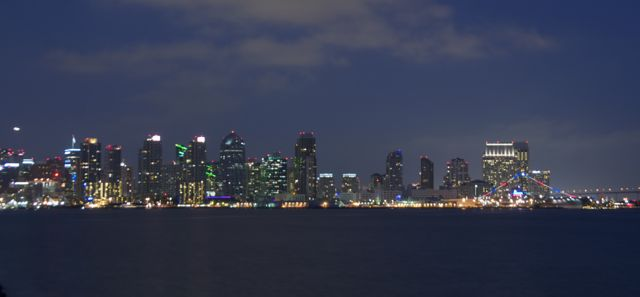
\includegraphics[width=0.5\textwidth]{sandiego}
  \caption[A picture of San Diego. Short figure caption must be \protect{$< 4$} lines in the list of figures]
{A picture of San Diego.  Short figure caption must be \protect{$< 4$} lines in the list of figures and match the start of the main figure caption verbatim. Note that figures must be on their own line (no neighboring text) and captions must be single-spaced and appear \protect\textit{below} the figure.  Captions can be as long as you want, but if they are longer than 4 lines in the list of figures, you must provide a short figure caption.\index{SanDiego}}
  \label{fig:sandiego}
\end{figure}

\subsection{A Table Example}

While in Section \ref{ssec:figure_example} Figure \ref{fig:sandiego} we had a majestic figure, here we provide a crazy table example.


%%%% TABLE 1 %%%%
\vspace{0.25in}
\begin{table}[!ht]
\caption[A table of when I get hungry.  Short table caption must be \protect{$< 4$} lines in the list of tables]{A table of when I get hungry. Short table caption must be \protect{$< 4$} lines in the list of tables and match the start of the main table caption verbatim.  Note that tables must be on their own line (no neighboring text) and captions must be single-spaced and appear \protect\textit{above} the table.  Captions can be as long as you want, but if they are longer than 4 lines in the list of figures, you must provide a short figure caption.}

\vspace{-0.25in}
\begin{center}
\begin{tabular}{|p{1in}|p{2in}|p{3in}|}

\hline
Time of day & Hunger Level & Preferred Food \\

\hline
8am & high & IHOP (French Toast) \\

\hline
noon & medium & Croutons (Tomato Basil Soup \& Granny Smith Chicken Salad) \\

\hline
5pm & high & Bombay Coast (Saag Paneer) or Hi Thai (Pad See Ew) \\

\hline
8pm & medium & Yogurt World (froyo!) \\

\hline
\end{tabular}
\end{center}
\label{tab:analysis3}
\end{table}

\chapter{Distributed Shared Persistent Memory}

\section{Introduction}
\label{sec:hotpot:introduction}

Next-generation non-volatile memories ({\em NVMs}), 
such as 3DXpoint~\cite{Intel3DXpoint}, 
phase change memory ({\em PCM}),
spin-transfer torque magnetic memories ({\em STTMs}),  and the memristor
will provide byte addressability, persistence, high density, and DRAM-like performance~\cite{NVMDB}.
These developments are poised to radically alter the landscape of memory and storage technologies
and have already inspired a host of research 
projects~\cite{Bailey10-OSImpl,Coburn11-ASPLOS, sosp09:bpfs, Dulloor14-EuroSys, hotos09:mogul, Volos11-ASPLOS, Xiaojian11-SC,Zhang15-Mojim,Octopus}.
However, most previous research on NVMs has focused on using them in a single machine environment.
Even though NVMs have the potential to greatly improve the performance and reliability of large-scale applications,
it is still unclear how to best utilize them in distributed, datacenter environments. 

This paper takes a significant step towards the goal of using NVMs in distributed datacenter environments.
We propose {\em Distributed Shared Persistent Memory (\dsnvm)},
a framework that provides a global, shared, and persistent memory space 
using a pool of machines with NVMs attached at the main memory bus.
Applications can perform native memory load and store instructions to access both local and remote data in this global memory space 
and can at the same time make their data persistent and reliable.
\dsnvm\ can benefit both single-node persistent-data applications that want to scale out efficiently
and shared-memory applications that want to add durability to their data.

Unlike traditional systems with separate memory and storage layers~\cite{Larchant,Perdis00,Larchant94,PerDis},
we propose to use just one layer that incorporates both distributed memory and 
distributed storage in \dsnvm.
\dsnvm's one-layer approach eliminates the performance overhead of data marshaling and unmarshaling,
and the space overhead of storing data twice. 
With this one-layer approach, \dsnvm\ can potentially provide the low-latency performance, 
vast persistent memory space, data reliability, and high availability
that many modern datacenter applications demand. 


Building a \dsnvm\ system presents its unique challenges.
Adding ``Persistence'' to Distributed Shared Memory (DSM)
is not as simple as just making in-memory data durable.
Apart from data durability, \dsnvm\ needs to provide two key features that DSM does not have:
persistent naming and data reliability.
In addition to accessing data in \nvm\ via native memory loads and stores,
applications should be able to easily
name, close, and re-open their in-memory data structures.
User data should also be reliably stored in NVM and sustain various types of failures; %(\eg, to have $N$ copies of persistent data).
they need to be consistent both within a node and across distributed nodes after crashes.
To make it more challenging, 
\dsnvm\ has to deliver these guarantees without sacrificing application performance
in order to preserve the low-latency performance of NVMs.

We built {\em \hotpot}, a \dsnvm\ system in the Linux kernel.
\hotpot\ offers low-latency, direct memory access, data persistence, reliability, and
high availability to datacenter applications.
It exposes a global virtual memory address space to each user application
and provides a new persistent naming mechanism that is both easy-to-use and efficient.
Internally, \hotpot\ organizes and manages data in a flexible way
and uses a set of adaptive resource management techniques to improve performance and scalability.

\hotpot\ builds on two main ideas to efficiently provide data reliability with distributed shared memory access.
Our first idea is to integrate distributed memory caching and data replication 
by imposing {\em morphable} states on persistent memory ({\em \nvm}) pages.

In DSM systems, when an application on a node accesses shared data in remote memory {\em on demand},
DSM caches these data copies in its local memory for fast accesses
and later evicts them when reclaiming local memory space.
Like DSM, \hotpot\ caches application-accessed data in local \nvm\
and ensures the coherence of multiple cached copies on different nodes.
But \hotpot\ also uses these cached data as {\em persistent data replicas}
and ensures their reliability and crash consistency.

On the other hand, unlike distributed storage systems, which {\em creates} extra data replicas 
to meet user-specified reliability requirements, 
\hotpot\ makes use of data copies that {\em already exist} in the system when
they were fetched to a local node due to application memory accesses.
 
In essence, every local copy of data serves two simultaneous purposes.
First, applications can access it locally without any network delay.
Second, by placing the fetched copy in \nvm, it can be treated as a persistent replica 
for data reliability.

This seemingly-straightforward integration is not simple. 
Maintaining wrong or outdated versions of data can result in inconsistent data.
To make it worse, these inconsistent data will be persistent in \nvm.
We carefully designed a set of protocols to deliver data reliability and crash consistency guarantees 
while integrating memory caching and data replication.

Our second idea is to exploit application behaviors and intentions in the \dsnvm\ setting. 
Unlike traditional memory-based applications, persistent-data-based applications,
\dsnvm's targeted type of application, have well-defined data {\em commit points}
where they specify what data they want to make persistent.
When a process in such an application makes data persistent,
it usually implies that the data can be {\em visible} outside the process (\eg, to other processes or other nodes). 
\hotpot\ utilizes these data commit points to also push updates to cached copies on distributed nodes
to avoid maintaining coherence on every \nvm\ write. %~\cite{XXX},
Doing so greatly improves the performance of \hotpot, 
while still ensuring correct memory sharing and data reliability.

To demonstrate the benefits of \hotpot, we ported the MongoDB~\cite{MongoDB} NoSQL database to \hotpot\
and built a distributed graph engine based on PowerGraph~\cite{Gonzalez12-OSDI} on \hotpot. 
Our MongoDB evaluation results show that \hotpot\ outperforms a \nvm-based replication system~\cite{Zhang15-Mojim} by up to 3.1\x{}, 
a recent \nvm-based distributed file systems~\cite{Octopus} by up to 3.0\x{}, and a DRAM-based file system by up to 53\x{}. 
\hotpot\ outperforms PowerGraph by 2.3\x{} to 5\x{}, a recent DSM system~\cite{Nelson15-ATC} by 1.3\x{} to 3.2\x{}.
Moreover, \hotpot\ delivers stronger data reliability and availability guarantees than these alternative systems.

Overall, this paper makes the following key contributions:

\begin{itemize}
\item We are the first to introduce the Distributed Shared Persistent Memory (DSPM) model
and among the first to build distributed \nvm-based systems.
The DSPM model provides direct and shared memory accesses to a distributed set of \nvm{}s 
and is an easy and efficient way for datacenter applications to use \nvm.

\item We propose a one-layer approach to build \dsnvm\ by 
integrating memory coherence and data replication.
The one-layer approach avoids the performance cost of two or more indirection layers.

\item We designed two distributed data commit protocols with different consistency levels 
and corresponding recovery protocols to 
ensure data durability, reliability, and availability.

\item We built the first \dsnvm\ system, \hotpot, in the Linux kernel, 
and two traditional kernel-level DSM systems (as comparison to \hotpot). 
\hotpot\ and the two DSM systems are both open sourced.

\item We demonstrated \hotpot's performance benefits and ease of use with two real datacenter applications
and extensive microbenchmark evaluation. 
We compared \hotpot\ with five existing file systems and distributed memory systems, 
and two in-house DSM systems.

\end{itemize}

The rest of the paper is organized as follows.
Section 2 presents and analyzes several recent datacenter trends that motivated our design of DSPM.
We discuss the benefits and challenges of DSPM in Section 3.
Section 4 presents the architecture and abstraction of Hotpot.
We then discuss Hotpot's data management in Section 5.
We present our protocols and mechanisms to ensure data durability, consistency, reliability, and availability in Section 6.
Section 7 briefly discusses the network layer we built underlying \hotpot,
and Section 8 presents detailed evaluation of Hotpot.
We cover related work in Section 9 and conclude in Section 10.

\hotpot\ is available at \url{https://github.com/WukLab/Hotpot}.
\section{Motivation}
\label{sec:motivation}

\dsnvm\ is motivated by three datacenter trends: 
emerging hardware \nvm\ technologies, 
modern data-intensive applications' data sharing, persistence, and reliability needs, 
and the availability of fast datacenter network.

\subsection{Persistent Memory and PM Apps}
Next-generation non-volatile memories ({\em NVMs}), 
such as 3DXpoint~\cite{Intel3DXpoint}, phase change memory ({\em PCM}),
spin-transfer torque magnetic memories ({\em STTMs}), and the memristor
will provide byte addressability, persistence, and latency that is within 
an order of magnitude of 
DRAM~\cite{hosomi2005novel,Lee10-pcmquest,lee2010phase,lee2011fast,qureshi2010morphable,NVMDB,yang2013memristive,Octopus}.
These developments are poised to radically alter the landscape of memory and storage technologies.

NVMs can attach directly to the main memory bus to form Persistent Memory, or \nvm. 
If applications want to exploit all the low latency and byte-addressability benefits of \nvm,
they should directly access it via memory load and store instructions without any software 
overheads~\cite{Coburn11-ASPLOS,Volos11-ASPLOS,Zhang15-Mojim,Memory-Persistency,Kamino-EuroSys17,pmxact-asplos16} 
(we call this model {\em durable in-memory computation}),
rather than accessing it via a file system~\cite{sosp09:bpfs,Dragojevic14-NSDI,Dulloor14-EuroSys,Xiaojian11-SC,HiNFS-Eurosys16,Octopus}.

{
\begin{figure}[th]
\begin{center}
\centerline{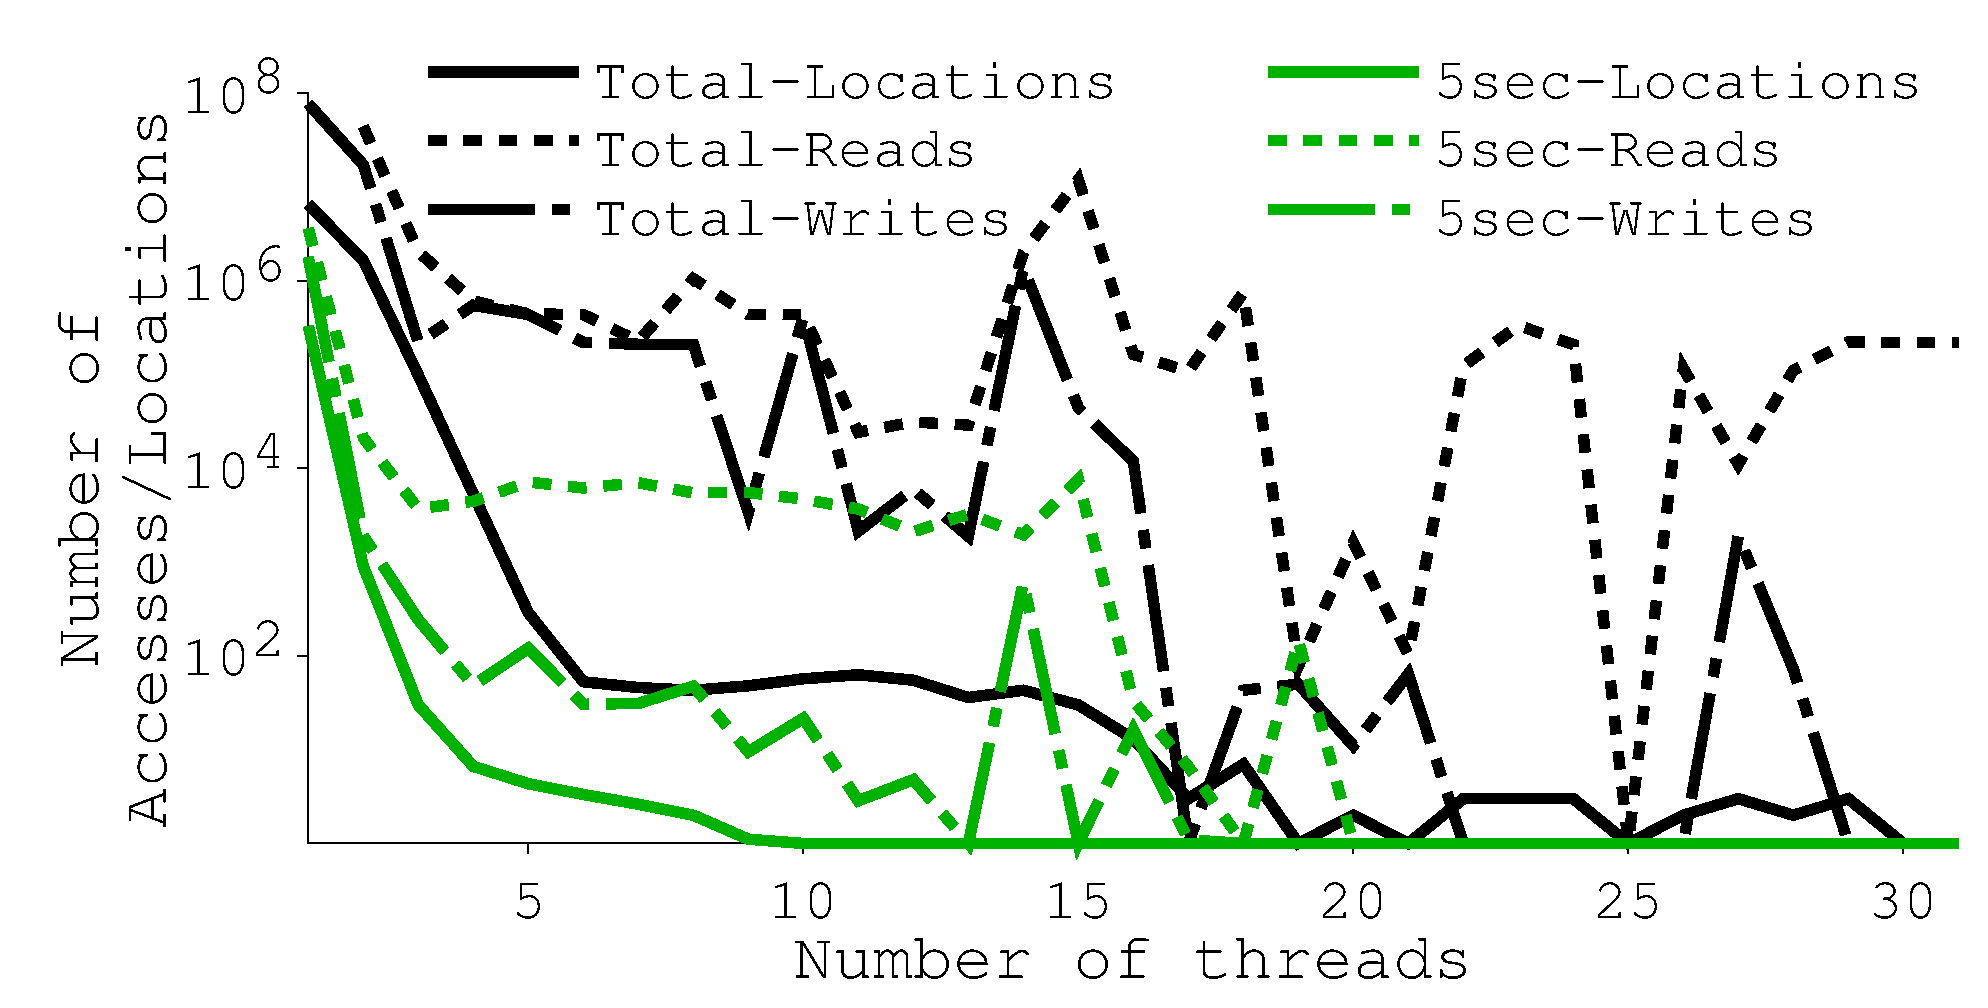
\includegraphics[width=0.4\textwidth]{Figures/g_plot_pagerank_average.pdf}}
\vspace{-0.15in}
\mycaption{fig-pagerank}{PowerGraph Sharing Analysis.}
{
Results of running PageRank~\cite{PageRank} on a Twitter graph~\cite{Kwak10-WWW}.
%Number of PowerGraph Pagerank memory reads and writes that are performed by $N$ threads to a shared location,
%and the number of such shared locations.
Black lines represent total amount of sharing.
Green lines represent sharing within five seconds.
}
\end{center}
\vspace{-0.2in}
\end{figure}
}

Unfortunately, most previous durable in-memory systems were designed for the single-node environment.
With modern datacenter applications' computation scale, 
we have to be able to scale out these single-node \nvm\ systems.

\subsection{Shared Memory Applications}
Modern data-intensive applications increasingly need
to access and share vast amounts of data fast. 
We use PIN~\cite{Luk05-PLDI} to collect memory access traces of two popular data-intensive applications, 
TensorFlow~\cite{TensorFlow} and PowerGraph~\cite{Gonzalez12-OSDI}.
Figures~\ref{fig-pagerank} and \ref{fig-tensorflow} show the total number of reads and writes performed to the same memory location 
by $N$ threads and the amount of these shared locations.
There are a significant amount of shared read accesses in these applications,
especially across a small set of threads.
We further divided the memory traces into smaller time windows 
and found that there is still a significant amount of sharing, 
indicating that many shared accesses occur at similar times. 

Distributed Shared Memory ({\em \dsm}) takes the shared memory concept a step further 
by organizing a pool of machines into a globally shared memory space.
Researchers and system builders have developed a host of software and hardware \dsm\ systems in the past few 
decades~\cite{Bennett90-PPOPP,Bisiani90-ISCA,Black89-COMPCON,Delp:1988:AIM:59505,Fleisch89-SOSP,Gibbons91-SPAA,Kontothanassis97-ISCA,Lo94-AC,Kessler89-ACM,Keleher92-ISCA,Ramachandran91-Wiley,Zhou92-IEEE,Stumm90-IEEE,Stumm90-IPDPS,HLRC,Shasta}.
Recently, there is a new interest in \dsm~\cite{Nelson15-ATC} to support modern data-intensive applications.

However, although DSM scales out shared-memory applications, 
there has been no persistent-memory support for DSM.
DSM systems all had to checkpoint to disks~\cite{Stumm90,Richard93,Neves94}.
Memory persistence
can allow these applications to checkpoint fast and recover fast~\cite{Narayanan12-ASPLOS}.

\subsection{Fast Network and RDMA}
Datacenter network performance has improved significantly over the past decades.
InfiniBand ({\em \ib}) NICs and switches support high bandwidth ranging from 40 to 100\gbps.
Remote Direct Memory Access ({\em RDMA}) technologies that provide low-latency remote memory accesses
have become more mature for datacenter uses in recent years~\cite{FaSST,Dragojevic14-NSDI,Kalia14-SIGCOMM,Guo16-SIGCOMM}.
These network technology advances
make remote-memory-based systems~\cite{Nelson15-ATC,GU17-NSDI,OSDI-Disaggregate,Chen16-EUROSYS,Binnig16-VLDB,Zamanian17-VLDB} more attractive than decades ago.

\subsection{Lack of Distributed PM Support}

{
\begin{figure}[t]
\begin{center}
\centerline{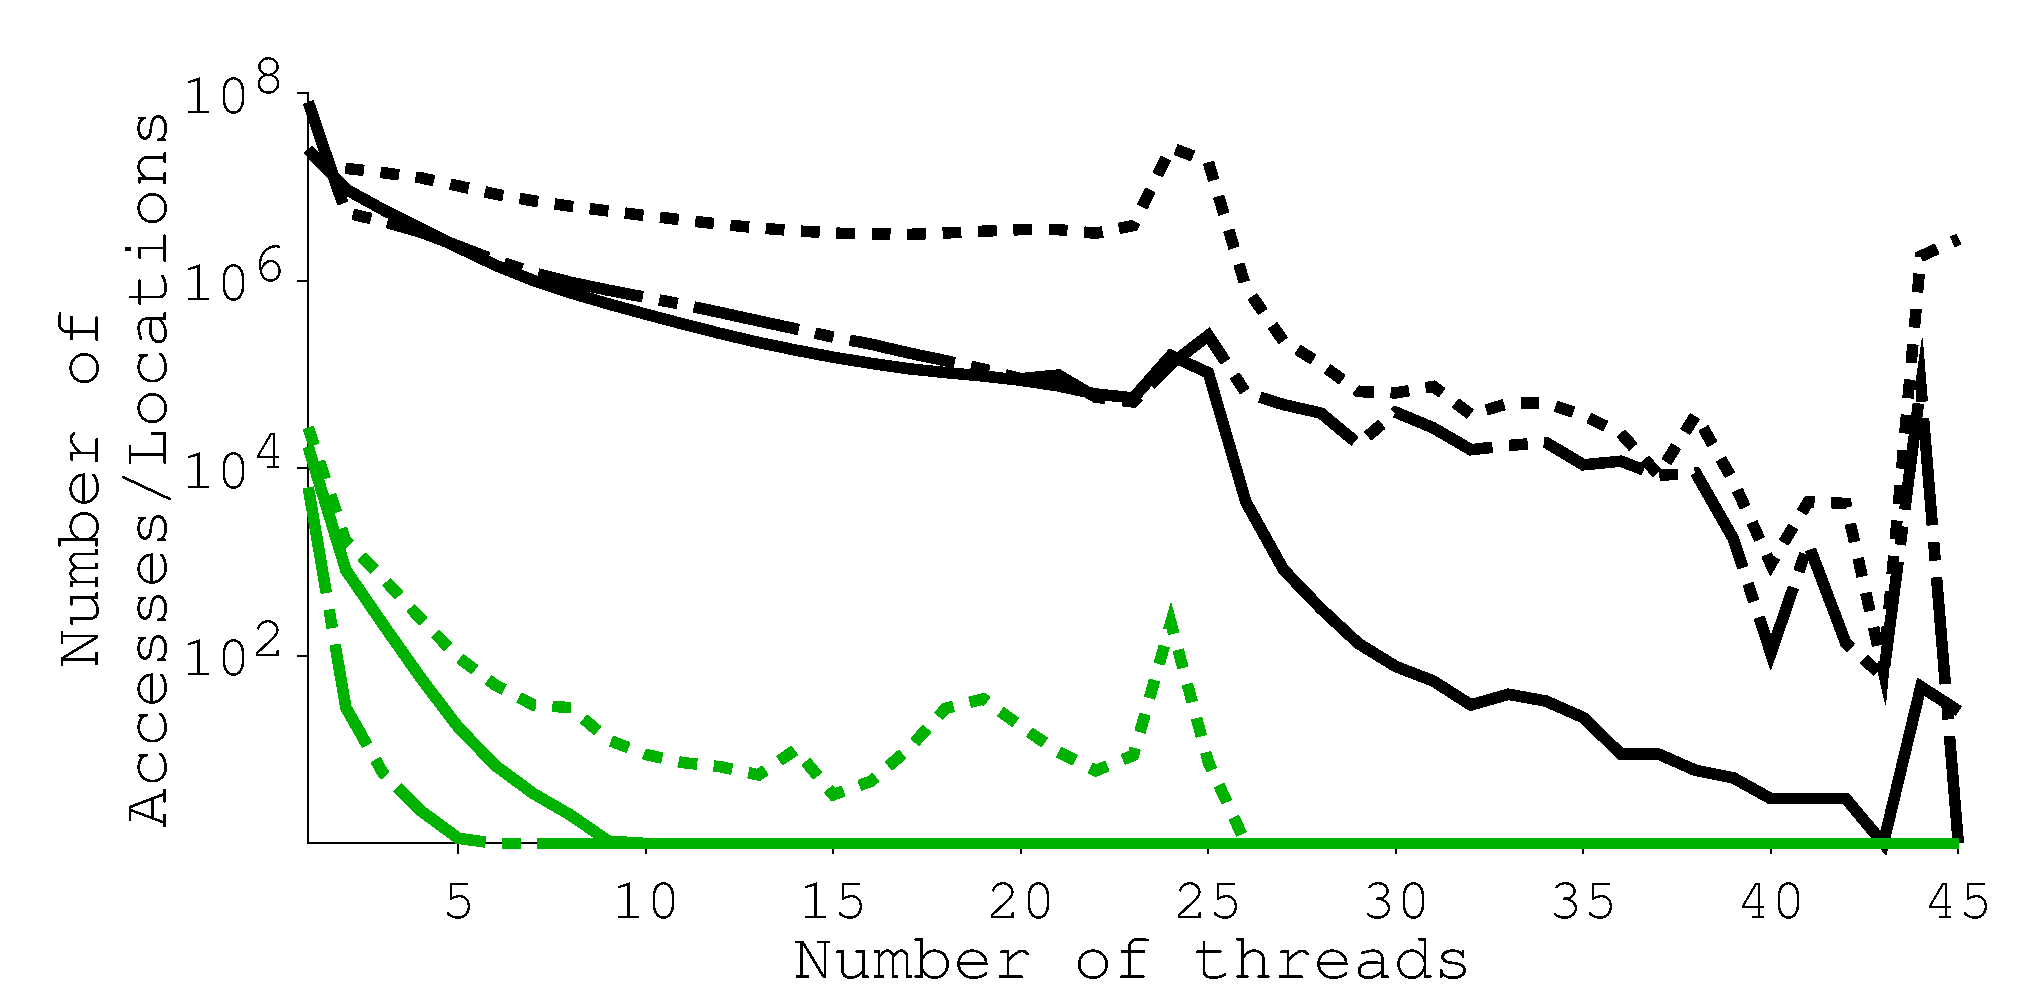
\includegraphics[width=\textwidth]{hotpot/Figures/g_plot_tensorflow_average.pdf}}
\caption[TensorFlow Sharing Analysis.]
{
TensorFlow Sharing Analysis.
Results of running a hand-writing recognition workloads provided by TensorFlow.
Black lines represent total amount of sharing.
Green lines represent sharing within five seconds.
}
\label{fig-tensorflow}
\end{center}
\end{figure}
}

Many large-scale datacenter applications require fast access to vast amounts of persistent data
and could benefit from \nvm's performance, durability, and capacity benefits.
For \nvm{}s to be successful in datacenter environments, they have to support these applications.
However, neither traditional distributed storage systems or DSM systems are designed for \nvm.
Traditional distributed storage systems~\cite{AdyaEtAl-Farsite,calder11-azure,DeCandia+07-Dynamo,Ghemawat03-GoogleFS,KubiEtAl00-Ocean,Petersen97-Bayou}
target slower, block-based storage devices.
Using them on \nvm{}s will result in excessive software and network overheads that outstrip \nvm's low latency performance~\cite{Zhang15-Mojim}.
DSM systems were designed for fast, byte-addressable memory, but lack the support for data durability and reliability.

Octopus~\cite{Octopus} is a recent RDMA-enabled distributed file system built for \nvm.
Octopus and our previous work Mojim~\cite{Zhang15-Mojim} are the only distributed \nvm-based systems that we are aware of.
Octopus was developed in parallel with \hotpot\ and has a similar goal as \hotpot: 
to manage and expose distributed PM to datacenter applications. 
However, Octopus uses a file system abstraction and is built in the user level.
These designs add significant performance overhead to native PM accesses (Section~\ref{sec:mongodb}).
Moreover, Octopus does not provide any data reliability or high availability, 
both of which are key requirements in datacenter environments.

\section{Distributed Shared Persistent Memory}
\label{sec:hotpot:dspm}

The datacenter application and hardware trends described in Section~\ref{sec:hotpot:motivation} 
clearly point to one promising direction of using \nvm\ in datacenter environments --- 
as distributed, shared, persistent memory (\dsnvm).
A \dsnvm\ system manages a distributed set of \nvm{}-equipped machines  
and provides the abstraction of a global virtual address space and a data persistence interface to applications.
This section gives a brief discussion on the \dsnvm\ model.

\subsection{\dsnvm\ Benefits and Usage Scenarios}
\dsnvm\ offers low-latency, shared access to vast amount of durable data in distributed \nvm,
and the reliability and high availability of these data.
Application developers can build in-memory data structures with the global virtual address space 
and decide how to name their data and when to make data persistent.

Applications that fit \dsnvm\ well have two properties:
accessing data with memory instructions and making data durable explicitly.
We call the time when an application makes its data persistent a {\em commit point}.
There are several types of datacenter applications that meet the above two descriptions and can benefit from running on \dsnvm.

First, applications that are built for single-node \nvm\
can be easily ported to \dsnvm\ and scale out to distributed environments.
These applications store persistent data as in-memory data structures 
and already express their commit points explicitly.
Similarly, storage applications that use memory-mapped files also fit \dsnvm\ well,
since they operate on in-memory data and explicitly make them persistent at well-defined commit points (\ie, \msync).
Finally, \dsnvm\ fits shared-memory or DSM-based applications that desire to incorporate durability.
These applications do not yet have durable data commit points,
but we expect that when developers want to make their applications durable, 
they should have the knowledge of when and what data they want make durable.

\subsection{\dsnvm\ Challenges}
\label{sec:hotpot:challenges}
Building a \dsnvm\ system presents several new challenges.

First, {\em what type of abstraction should \dsnvm\ offer to support both direct memory accesses and data persistence (Section~\ref{sec:hotpot:abstraction})}?
To perform native memory accesses, application processes should use virtual memory addresses. 
But virtual memory addresses are not a good way to {\em name} persistent data.
\dsnvm\ needs a naming mechanism that applications can easily use to retrieve their in-memory data after reboot or crashes (Section~\ref{sec:hotpot:naming}).
Allowing direct memory accesses to \dsnvm\ also brings another new problem:
pointers need to be both persistent in \nvm\ and consistent across machines (Section~\ref{sec:hotpot:addressing}).

Second, {\em how to efficiently organize data in \dsnvm\ to deliver good application performance (Section~\ref{sec:hotpot:data})?}
To make \dsnvm's interface easy to use and transparent, 
\dsnvm\ should manage the physical \nvm\ space for applications and handle \nvm\ allocation.
\dsnvm\ needs a flexible and efficient data management mechanism to deliver good performance to different types of applications.

Finally, {\em \dsnvm\ needs to ensure both distributed cache coherence and data reliability at the same time} (Section~\ref{sec:hotpot:xact}).
The former requirement ensures the coherence of multiple cached copies at different machines under concurrent accesses and is usually enforced in a distributed memory layer.
The latter provides data reliability and availability when crashes happen and is implemented in distributed storage systems or distributed databases.
\dsnvm\ needs to incorporate both these two different requirements in one layer in a correct and efficient way.
%Note that PM is attached to main memory bus directly, hence we assume PM share the same CPU cache coherence mechanism with DRAM.
%Hotpot focus on cache coherence among different cached copies across nodes.

\section{\hotpot\ Architecture and Abstraction}
\label{sec:design}
\label{sec:abstraction}

We built {\em \hotpot}, a kernel-level \dsnvm\ system that %manages \dsnvm\ and
%manages distributed shared persistent memory
provides applications with direct memory load/store access to both local and remote \nvm\
and a mechanism to make in-\nvm\ data durable, consistent, and reliable.
\hotpot\ is easy to use, delivers low-latency performance, 
and provides flexible choices of data consistency, reliability, and availability levels.
This section presents the overall architecture of \hotpot\ and its abstraction to applications.

We built most of \hotpot\ as a loadable kernel module in Linux 3.11.0 
with only a few small changes to the original kernel. 
\hotpot\ has around 19K lines of code, out of which 6.4K lines are for a customized network stack (Section~\ref{sec:network}).
\hotpot\ is available at {\url https://github.com/WukLab/Hotpot}.

\if 0
This section describes \hotpot's overall architecture and abstraction,
how \hotpot\ manages user data and its own metadata, 
\hotpot's data consistency and reliability solutions,
and \hotpot's resource management mechanisms and network layer.
\fi

\hotpot\ sits in the kernel space and manages \nvm{}s in a set of distributed nodes, or {\em \hotpot\ nodes}.
\hotpot\ provides applications with an easy-to-use, memory-based abstraction that encapsulates 
both memory and persistent data access in a transparent way.
Figure~\ref{fig-architecture} presents \hotpot's architecture.
\hotpot\ uses a {\em Central Dispatcher (\cd)} 
to manage node membership and initialization tasks (\eg, create a dataset).
All data and metadata communication after a dataset has been created takes place between \hotpot\ nodes and does not involve the \cd.

{
\begin{figure*}[th]
\begin{subfigure}{1.7in}
\begin{center}
\centerline{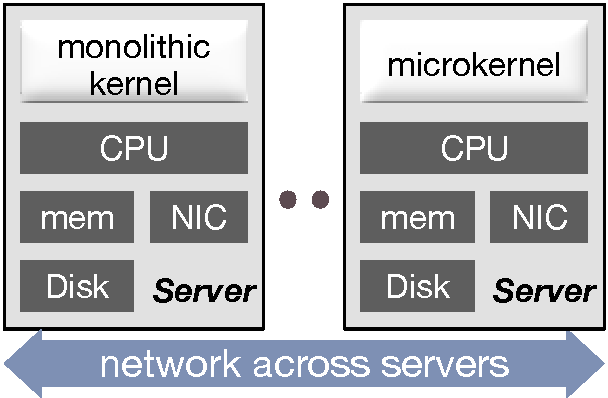
\includegraphics[width=1.7in]{lego/Figures/monolithic-arch.pdf}}
\caption[Monolithic OS.]{OSes Designed for Monolithic Servers.}
\label{fig-monolithic}
\end{center}
\end{subfigure}
\begin{minipage}{0.05in}
\hspace{0.05in}
\end{minipage}
\begin{subfigure}{1.8in}
\begin{center}
\centerline{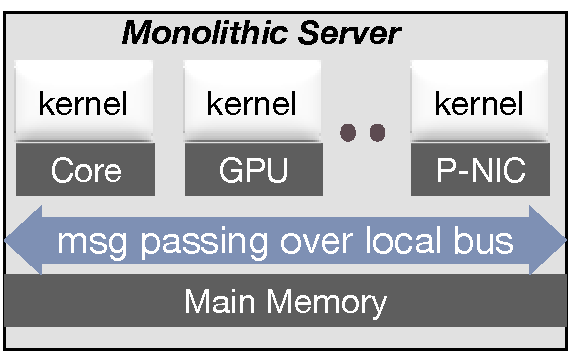
\includegraphics[width=1.8in]{lego/Figures/multikernel-arch.pdf}}
\caption[Multikernel Architecture.]{Multi-kernel Architecture. \small{P-NIC: programmable NIC.}}
\label{fig-multikernel}
\end{center}
\end{subfigure}
\begin{minipage}{0.05in}
\hspace{0.05in}
\end{minipage}
\begin{subfigure}{2.5in}
\begin{center}
\centerline{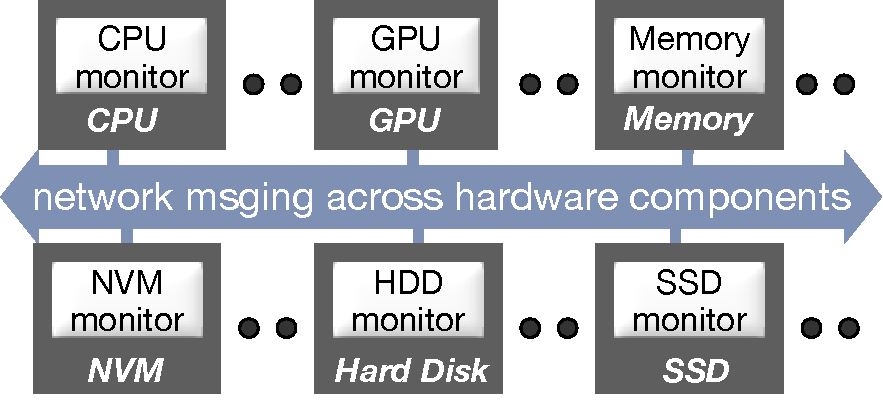
\includegraphics[width=2.6in]{lego/Figures/lego-arch.pdf}}
\caption[Splitkernel Architecture.]{Splitkernel Architecture.}
\label{fig-splitkernel}
\end{center}
\end{subfigure}
\caption[Operating System Architecture.]{Operating System Architecture.}
\end{figure*}
}

\subsection{Application Execution and Data Access Abstraction}
Most data-intensive applications are multithreaded 
and distribute their data processing work across threads~\cite{MongoDB,Gonzalez12-OSDI}.
Thus, \hotpot\ adopts a thread-based model to run applications on a set of \hotpot\ nodes.
\hotpot\ uses application threads as the unit of deployment and
lets applications decide what operations and what data accesses they want to include in each thread.
Applications specify what threads to run on each \hotpot\ node 
and \hotpot\ runs an application by starting all its threads together on all \hotpot\ nodes. 
We give users full flexibility in choosing their initial thread and workload distributions.
However, such user-chosen distributions may not be optimal, especially as workloads change over time.
To remedy this situation, 
\hotpot\ provides a mechanism to adaptively move data closer to computation based on workload behavior, 
as will be discussed in Section~\ref{sec:migration}.


\hotpot\ provides a global virtual memory address space to each application.
Application threads running on a node can perform native memory load and store instructions using global virtual memory addresses 
to access both local and remote \nvm.
The applications do not know where their data physically is or whether a memory access is local or remote.
Internally, a virtual memory address can map to a local physical page if the page exists locally or 
generate a page fault which will be fulfilled by \hotpot\ by fetching a remote page (more in Section \ref{sec:readwrite}). 
Figure~\ref{fig-addressing} presents an example of \hotpot's global virtual address space.
Unlike an I/O-based interface, \hotpot's native memory interface can best exploit \nvm{}s' low-latency, DRAM-like performance, and byte addressability.

On top of the memory load/store interfaces, \hotpot\ provides a mechanism for applications to 
name their data,
APIs to make their data persistent, %: \beginxact, \commitxact, and \commit,
and helper functions for distributed thread synchronization. 
%We will discuss these three APIs in detail in Section~~\ref{sec:xact}.
Table~\ref{tbl-apis} lists \hotpot\ APIs.
We also illustrate \hotpot's programming model with a simple program in Figure~\ref{fig-code-eg}.
We will explain \hotpot's data commit semantics in Section~\ref{sec:xact}.

{
\begin{table}[t]\normalsize
\begin{center}
\caption[\hotpot\ APIs.]{
Apart from these APIs, \hotpot\ also supports direct memory loads and stores.
}
\begin{center}
\begin{tabular} { p{1.2in} | p{2.5in} | p{1.8in} }
\normalsize API & \normalsize Explanation & \normalsize Backward \\
\hline
\hline
\open\ \ \ \ (\close) & open or create (close) a \dsnvm\ dataset & same as current \\
\hline
\mmap\ (\unmap) & map (unmap) a \dsnvm\ region in a dataset to application address space & same as current \\
%\close\ & close a \dsnvm\ dataset & same as file \close\ \\
\hline
\commit\  & commit a set of data and make $N$ persistent replicas & similar to msync \\
\hline
\acquire\  & acquire single writer permission & \\
%\fetch\ & fetch a set of committed data & \\
\hline
%\commit\ & atomically commit dirty data and make $N$ persistent replicas & same as current \\
%\hline
\barrier\ & helper function to synchronize threads on different nodes & similar to pthread barrier \\
\end{tabular}
\end{center}
\label{tbl-apis}
\end{center}
\end{table}
}
{
\begin{figure}[th]
\begin{center}
\centerline{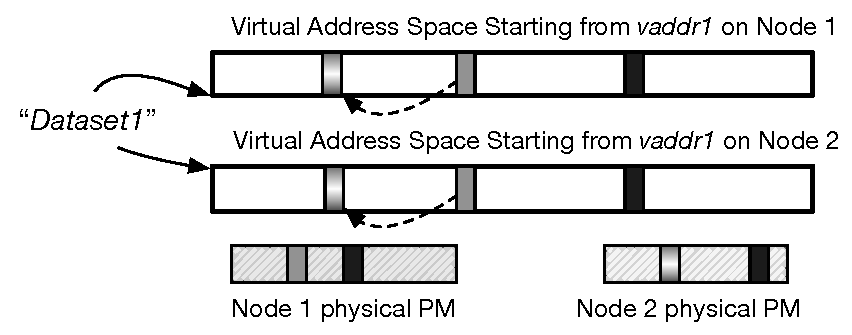
\includegraphics[width=\textwidth]{hotpot/Figures/addressing.pdf}}
\caption[\hotpot\ Addressing.]
{\hotpot\ Addressing.
\hotpot\ maps ``{\em Dataset1}'' to Node 1 and Node 2's virtual address space using the 
same base virtual addresses. The physical address mapping on each node is different.
The grey blocks in the middle are pointers that point to the blocks on the left. 
}
\label{fig-hotpot-addressing}
\end{center}
\end{figure}
}

\subsection{Persistent Naming}
\label{sec:naming}
To be able to store persistent data and to allow applications to re-open them after closing or failures, 
\hotpot\ needs to provide a naming mechanism that can sustain power recycles and crashes. 

Many modern data-intensive applications such as in-memory databases~\cite{MongoDB} and graphs~\cite{Gonzalez14-OSDI,Gonzalez12-OSDI}
work with only one or a few big datasets that include all of an application's data 
and then manage their own fine-grained data structures within these datasets.
Thus, instead of traditional hierarchical file naming, 
we adopt a flat naming mechanism in \hotpot\ to reduce metadata management overhead. % to let applications name their persistent data in \dsnvm.

Specifically, \hotpot\ applications assign names by {\em datasets}
and can use these names to open the datasets.
A dataset is similar to the traditional file concept, 
but \hotpot\ places all datasets directly under a mounted \hotpot\ partition without any directories or hierarchies.
Since under \hotpot's targeted application usage, there will only be a few big datasets,
dataset lookup and metadata management with \hotpot's flat namespace are easy and efficient.
We use a simple (persistent) hash table internally to lookup datasets. 

The \open\ and \mmap\ APIs in Table~\ref{tbl-apis} let applications create or open a dataset with a name and 
map it into the application's virtual memory address space.
Afterwards, all data access is through native memory instructions.

{
\begin{figure}[th]
\begin{center}
\scriptsize
\lstinputlisting[
language=C
]{hotpot/code-eg.c}
\caption[Sample code using \hotpot.]{Sample code using \hotpot.}
\label{fig-code-eg}
\end{center}
\end{figure}
}


\subsection{Consistent and Persistent Pointers} 
\label{sec:addressing}

\hotpot\ applications can use \dsnvm\ as memory and store arbitrary data structures in it. 
One resulting challenge is the management of pointers in \dsnvm.
To make it easy to build persistent applications with memory semantics, 
\hotpot\ ensures that pointers in \dsnvm\ have the same value (\ie, virtual addresses of the data that they point to) 
both across nodes and across crashes. 
Application threads on different \hotpot\ nodes can use pointers directly without pointer marshaling or unmarshaling,
even after power failure.
We call such pointers {\em globally-consistent and persistent pointers}.
Similar to NV-Heaps~\cite{Coburn11-ASPLOS}, we restrict \dsnvm\ pointers to only point to data within the same dataset. 
Our targeted type of applications which build their internal data structures within big datasets already meet this requirement.

To support globally-consistent and persistent pointers, 
\hotpot\ guarantees that the same virtual memory address is used as the starting address of a dataset across nodes and across re-opens of the dataset.
With the same base virtual address of a dataset and virtual addresses within a dataset being consecutive, 
all pointers across \hotpot\ nodes will have the same value. 

We developed a new mechanism to guarantee that the same base virtual address is used across nodes and crashes.
When an application opens a dataset for the first time, \hotpot\ uses a consensus protocol to discover the current 
available virtual address ranges on all nodes and select one for the dataset. 
Nodes that have not opened the dataset will reserve this virtual address range for possible future opening of the dataset.
Since the total amount of virtual addresses for \dsnvm\ is bound to the total size of \dsnvm\ datasets, 
\hotpot\ can always find available virtual address ranges on 64-bit platforms.
\hotpot\ records the virtual address range persistently and forces applications to use the same virtual address 
the next time it starts.
To ensure that recorded persistent virtual address ranges are always available when opening datasets, 
we change the kernel loader and virtual memory address allocator (\ie, {\it brk} implementation) to exclude 
all recorded address ranges.

\section{Data Management and Access}
\label{sec:hotpot:data}

This section presents how \hotpot\ manages user data in \dsnvm. 
We postpone the discussion of data durability and reliability to Section~\ref{sec:hotpot:xact}.

\subsection{\nvm\ Page Morphable States}
One of \hotpot's design philosophies is to use one layer for both memory and storage 
and to integrate distributed memory caching and data replication.
To achieve this goal, we propose to impose {\em morphable} states on \nvm\ pages,
where the same \nvm\ page in \hotpot\ can be used both as a local memory cached copy to improve performance
and as a redundant data page to improve data reliability and availability.

We differentiate three states of a \nvm\ page:
active and dirty, active and clean, and inactive and clean,
and we call these three states {\em \dirty}, {\em \committed}, and {\em \redundant} respectively.
A page being clean means that it has not been updated since the last commit point;
committing a dirty page moves it to the clean state.
A page being active means that it is currently being accessed by an application,
while an \redundant\ page is a page which the application process has not mapped or accessed.
Several \hotpot\ tasks can change page states,
including page read, page write, data commit, data replication, page migration, and page eviction.
We will discuss how page states change throughout the rest of this section.
Figure~\ref{fig-data-eg} illustrates two operations that cause \hotpot\ data state changes.

\subsection{Data Organization}
\hotpot\ aims to support large-scale, data-intensive applications
on a fairly large number of nodes. %(\eg, at least a few racks)
Thus, it is important to minimize \hotpot's performance and scalability bottlenecks.
In order to enable flexible load balancing and resource management,
\hotpot\ splits the virtual address range of each dataset 
into {\em chunks} of a configurable size (\eg, 4\MB).
\nvm\ pages in a chunk do not need to be physically consecutive
and not all pages in a chunk need to exist on a node.

Each chunk in \hotpot\ is owned by an {\em owner node (\on)},
similar to the ``home'' node in home-based DSM systems~\cite{HLRC}.
%and to the primary node of distributed storage systems,
An \on\ maintains all the data and metadata of the chunk it owns.
%and serves requests from other nodes.
Other nodes, called {\em data node} or {\em \dn}, always fetch data from the \on\
when they initially access the data.
A single \hotpot\ node can simultaneously be the \on\ for some data chunks and the \dn\ for other chunks.
When the application creates a dataset, 
\hotpot\ \cd\ performs an initial assignment of \on{}s to chunks of the dataset.

Two properties separate \hotpot\ \on{}s from traditional home nodes.
First, %besides serving read data,
\hotpot\ \on\ is responsible for the reliability and crash consistency of the pages it owns,
besides serving read data and ensure the coherence of cached copies.
Second, \hotpot\ does not fix which node owns a chunk
and the location of \on\ adapts to application workload behavior dynamically.
Such flexibility is important for load balancing and application performance (see Section~\ref{sec:hotpot:migration}).

\subsection{Data Reads and Writes}
\label{sec:hotpot:readwrite}

\hotpot\ minimizes software overhead to improve application performance.
It is invoked only when a page fault occurs or when 
applications execute data persistence operations (see Section~\ref{sec:hotpot:xact} for details of data persistence operations).

{
\begin{figure}[th]
\centering
\begin{center}
\centerline{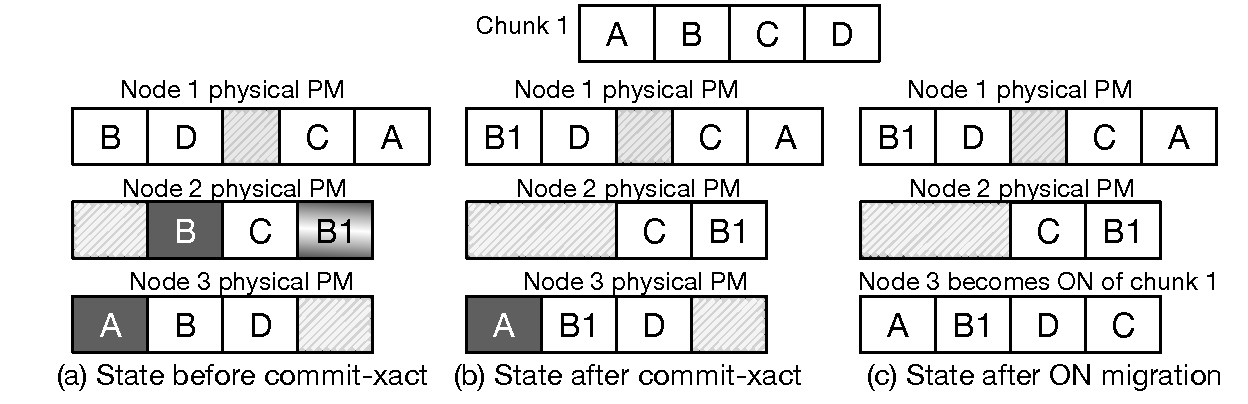
\includegraphics[width=\textwidth]{hotpot/Figures/data-eg.pdf}}
\end{center}
\caption[Data State Change Example.]
{Data State Change Example.
White, black, and striped blocks represent \committed, \redundant, and \dirty\ states.
Before commit, Node 2 and Node 3 both have cached copies of 
data page $B$. Node 2 has written to $B$ and created a \dirty\ page, $B1$.
During commit, Node 2 pushes the content $B1$ to its \on, Node 1.
Node 1 updates its \committed\ copy to $B1$ and also sends this update to Node 3.
Figure (c) shows the state after migrating the \on\ of chunk 1 from Node 1 to Node 3. 
After migration, Node 3 has all the pages of the chunk and all of them are in \committed\ states.
}
\label{fig-data-eg}
\end{figure}
}
When a page fault happens because of read, 
it means that there is no valid local page.
\hotpot\ first checks if there is any local \redundant\ page.
If so, it will move this page to the \committed\ state and establish a page table entry (PTE) for it.
Otherwise, there is no available local data and 
\hotpot\ will fetch it from the remote \on.
\hotpot\ writes the received data to a newly-allocated local physical \nvm\ page.
Afterwards, applications will use memory instructions to access this local page directly.


Writing to a \committed\ page also causes a page fault in \hotpot. 
This is because a \committed\ page can contribute towards user-specified degree of replication as one data replica,
and \hotpot\ needs to protect this committed version from being modified.
Thus, \hotpot\ write protects all \committed\ pages.
When these pages are written to (and generating a write page fault), 
\hotpot\ creates a local Copy-On-Write (COW) page
and marks the new page as dirty while leaving
the original page in \committed\ state.
\hotpot\ does not write protect this COW page, since it is already in the dirty state.

Following \hotpot's design philosophy to exploit hints from our targeted data-intensive applications,
we avoid propagating updates to cached copies at other nodes on each write and only do so at each application commit point.
Thus, all writes in \hotpot\ is local and only writing to a \committed\ page will generate a page fault.

Not updating remote cached copies on each write also has the benefit of reducing write amplification in \nvm.
In general, other software mechanisms and policies such as wear-aware \nvm\ allocation and reclamation 
and hardware techniques like Start-Gap~\cite{start-gap-micro09}
can further reduce \nvm\ wear.
We do not focus on \nvm\ wear in this paper and leave such optimizations for future work.

\subsection{\nvm\ Page Allocation and Eviction}
\label{sec:hotpot:eviction}
Each \hotpot\ node manages its own physical \nvm\ space and performs \nvm\ page allocation and eviction.
Since physical pages do not need to be consecutive,
we use a simple and efficient allocation mechanism by maintaining a free page list
and allocating one page at a time.

\hotpot\ uses an approximate-LRU replacement algorithm that is similar to Linux's page replacement mechanism.
Different from Linux,
\hotpot\ distinguishes pages of different states.
\hotpot\ never evicts a \dirty\ page
and always tries to evict \redundant\ pages before evicting \committed\ pages.
We choose to first evict \redundant\ pages, 
because these are the pages that have not been accessed by applications
and less likely to be accessed in the future than \committed\ pages. %if a node accesses an \redundant\ page, it will become an \committed\ page.

Since both \redundant\ and \committed\ pages can serve as a redundant copy
for data reliability, \hotpot\ cannot simply throw them away during eviction.
The evicting node of a page will contact its \on{}, 
which will check the current degree of replication of the candidate pages 
and prioritize the eviction of pages that already have enough replicas. 
For pages that will drop below the user-defined replication degree after the eviction, 
the \on\ will make a new \redundant\ page at another node. %, if the eviction violates user-specified reliability requirements.

\subsection{Chunk \on\ Migration}
\label{sec:hotpot:migration}
An \on{} serves both page read and data commit requests that belong to the chunks it owns.
Thus, the location of \on\ is important to \hotpot's performance.
Ideally, the node that performs the most reads and commits of data in a chunk 
should be its \on\ to avoid network communication.

By default, \hotpot\ initially spreads out a dataset's chunks to all \hotpot\ nodes in a round robin fashion
(other static placement policies can easily replace round robin).
Static placement alone cannot achieve optimal run-time performance.
\hotpot\ remedies this limitation by performing online chunk migration,
where one \on\ and one \dn\ of a chunk can switch their identities
and become the new \dn\ and new \on\ of the chunk.

\hotpot\ utilizes application behavior in recent history 
to decide how to migrate \on{}s.
Each \on\ records the number of page read requests
and the amount of committing data it receives in the most recent time window.

\on{}s make their migration decisions with a simple greedy algorithm based on the combination of two criteria:
maximizing the {\em benefit} while not exceeding a configurable {\em cost} of migration.
The benefit is the potential reduction in network traffic during remote data reads and commits.
The node that performs most data communication to the \on\ in recent history
is likely to benefit the most from being the new \on,
since after migration these operations will become local.
We model the cost of migration by the amount of data needed to copy to a node so that it has all the chunk data to become \on.

Once \hotpot\ has made a decision, it performs the actual chunk migration using 
a similar method as process and VM migration~\cite{OsmanEtAl02-Zap,Douglis87-Migration,Clark05-XenMigrate}
by temporary stopping commits to the chunk under migration
and resume them at the new \on\ after migration.

\if 0
    Once decided, a new ON node will be chosen. And the old ON will start to migrate pages to the
    the ON. During migration, the old ON is still the only valid ON in system. And, the old ON
    will keep serving page-fetch, but xact will be rejected.

    Once all pages are migrated from old ON to new ON, the old ON will 1) Tell CD that this region
    is migrated, hence CD can change its metadata. 2) Broadcast to nodes that currently have this
    region, that this region is migrated to new ON.
\fi

\if 0
\subsubsection{Replica Selection}
Apart from \on\ locations, the locations of data replicas can also affect application performance.
When a node has an \redundant\ page it can directly access it and avoid a remote page read. 
Thus, placing a data replica at a node that is likely to access the data in the future
can potentially improve performance.

\hotpot\ \on\ decides where to place an \redundant\ page during transaction commit with two criteria. 
%Currently, we use two criteria in selecting the location of a replica.
%replication gives us a chance to re-balance workloads
%happened in two occasions:
%when committing a transaction 
%and when evicting a \redundant\ page.
First, we use spatial locality to estimate the likelihood a node is going to access an \redundant\ page 
by the number of pages this node has read in the chunk that contains the \redundant\ page.
The second consideration is to prevent thrashing.
When a node runs out of space, it will first evict \redundant\ pages (Section~\ref{sec:hotpot:eviction})
and assigning \redundant\ pages to such nodes will cause thrashing.
Thus, \hotpot\ compares the total \nvm\ free space of a node and avoids assigning 
\redundant\ pages to nodes with space pressure.
\fi

\section{Data Durability, Consistency, and Reliability}
\label{sec:hotpot:xact}

Being distributed shared memory and distributed storage at the same time,
\dsnvm\ should ensure both correct shared memory accesses to \nvm\
and the persistence and reliability of in-\nvm\ data. 
\hotpot\ provides three guarantees: coherence among cached copies of in-\nvm\ data,
recovery from various types of failures into a consistent state,
and user data reliability and availability under concurrent failures.
Although each of these three properties have been explored before,
as far as we know, \hotpot\ is the first system that integrates all of them in one layer.
\hotpot\ also has the unique requirement of low software overhead to retain the performance benefit of \nvm.

\begin{itemize}
\item{\em Cache coherence.} 
In \hotpot, application processes on different nodes cache remote data in their local \nvm\ for fast accesses.
\hotpot\ provides two consistency levels across cached copies: 
{\em \ra}, multiple readers and single writer ({\em MRSW}) 
and {\em \rb}, multiple readers and multiple writers ({\em MRMW}).
MRMW allows multiple nodes to concurrently write and commit their local cached copies.
With \mrmw, there can be multiple versions of dirty data in the system (but still one committed version),
while \mrsw\ guarantees only one dirty version at any time.
An application can use different modes for different datasets,
but only one mode with the same dataset.
This design allows flexibility at the dataset granularity while guaranteeing correctness.
 
\item{\em Crash consistency.} 
Data storage applications usually have well-defined {\em consistent} states and need to move from 
one consistent state to another atomically.
When a crash happens, 
user data should be recovered to a consistent state ({\ie, \em crash consistency}). 
\hotpot\ guarantees crash consistency both within a single node ({\em \rcs}) and across distributed nodes ({\em \rcm}).
Note that crash consistency is different and orthogonal to cache
coherence in \ra\ and \rb. 

\item{\em Reliability and availability.} 
To ensure that user persistent data can sustain $N-1$ concurrent node failures, 
where $N$ is a user defined value, \hotpot\ guarantees that {\em \re}, once data has 
been committed, there are always $N$ copies of clean, committed data.

\end{itemize}

This section first discusses how \hotpot\ ensures crash consistency within a single node,
then presents the \mrmw\ and \mrsw\ modes and their atomic commit protocols, %and the optional group fetch protocol.
and ends with the discussion of \hotpot's recovery mechanisms under different crash scenarios.

\subsection{Single-Node Persistence and Consistency}
\label{sec:hotpot:singleconsistency}

Before ensuring user data's global reliability and consistency in \dsnvm,
\hotpot\ first needs to make sure that data on a single node can properly sustain power crashes (\rcs)~\cite{Memory-Persistency}.
\hotpot\ makes data persistent with the standard Intel persistent memory instructions~\cite{Delegated-persist},
\ie, \clflush, \mfence\ (note that we do not include the deprecated \pcommit\ instruction~\cite{Deprecating-PCOMMIT}).

After a node crashes, if its \nvm\ is still accessible, \hotpot\ will use the \nvm\ content to recover;
otherwise, \hotpot\ will use other nodes to reconstruct data on a new node (Section~\ref{sec:hotpot:recovery}).
For the former case, \hotpot\ needs to guarantee that user data in \dsnvm\ is in a consistent state after crash.
\hotpot\ also needs to ensure that its own metadata is persistent and is consistent with user data.

\hotpot\ maintains metadata on a local node to find user data and record their morphable states (\ie, \committed, \dirty, or \redundant).
Since these metadata are only used within a single node, \hotpot\ does not need to replicate them on other nodes.
\hotpot\ makes these metadata persistent at known locations in \nvm\ ---
a pre-allocated beginning area of \nvm.
\hotpot\ also uses metadata to record online state of the system (\eg, \on\ maintains a list of active \dn{}s that have a cached copy of data).
These metadata can be reconstructed by re-examining system states after recovery.
Thus, \hotpot\ does not make these metadata persistent.

Similar to traditional file systems and databases, 
it is important to enforce {\em ordering} of metadata and data persistence
in order to recover to a consistent state.
For single-node non-commit operations (we defer the discussion of commit operations to Sections \ref{sec:hotpot:mrmw} and \ref{sec:hotpot:mrsw}), 
\hotpot\ uses a simple shadow-paging mechanism to ensure that the consistency of metadata and data.
Specifically, we associate each physical memory page with a metadata slot
and use a single 8-byte index value to locate both the physical page and its metadata.
When an application performs a memory store to a \committed\ page,
\hotpot\ allocates a new physical page, writes the new data to it, and writes the new metadata 
(\eg, the state of the new page) to the metadata slot associated with this physical page.
After making all the above data and metadata persistent, \hotpot\ changes the index
from pointing to the old \committed\ page to pointing to the new \dirty\ page.
Since most architectures support atomic 8-byte writes, this operation atomically moves the system to a new consistent state with both the new data and the new metadata.
%and \hotpot\ can always recover local data to a consistent state after crashes.

{
\begin{figure}[t]
\begin{center}
\centerline{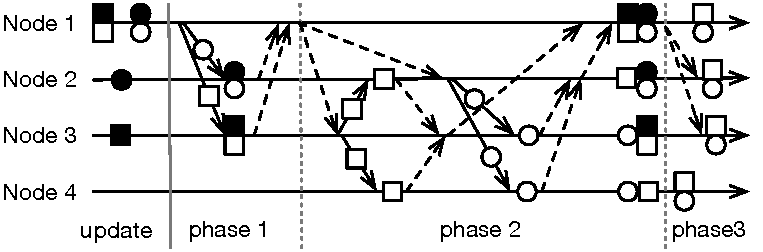
\includegraphics[width=\textwidth]{hotpot/Figures/commit.pdf}}
\caption[\mrmw\ Commit Example.]
{
\mrmw\ Commit Example.
Solid arrows represent data communication.
Dashed arrows represent metadata communication.
Node 1 (\xn) commit data to \on{}s at Node 2 and 3 with replication degree four.
Black shapes represent old committed states before the update
and white shapes represent new states.
}
\label{fig-mrmw}
\end{center}
\end{figure}
}

\subsection{\mrmw\ Mode}
\label{sec:hotpot:mrmw}
\hotpot\ supports two levels of concurrent shared-\nvm\ accesses and uses different protocols to commit data.
The \mrmw\ mode allows multiple concurrent versions of dirty, uncommitted data 
to support great parallelism.
\mrmw\ meets \rb, \rcm, and \re.

\mrmw\ uses a distributed atomic commit protocol at each commit point %(a user \commit\ call)
to make local updates globally visible, persistent, and replicated.
Since \mrmw\ supports concurrent commit operations 
and each commit operation can involve multiple remote \on{}s,
\hotpot\ needs to ensure that all the \on{}s reach consensus on the commit operation they serve. 
We designed a three-phase commit protocol for the \mrmw\ mode
based on traditional two-phase commit protocols~\cite{Samaras93,Gray78,Lampson81} but differs in that
\hotpot\ needs to ensure cache coherence, crash consistency, and data replication all in one protocol.
Figure~\ref{fig-mrmw} illustrates an example of \mrmw. 

{\bf Commit phase 1.} 
When a node receives a \commitxact\ call (we call this node {\em \xn}), it checks if data specified in the \commitxact\ call is dirty
and commits only the dirty pages.
\xn\ persistently records the addresses of these dirty pages for recovery reasons (Section~\ref{sec:hotpot:recovery}).
\xn\ also assigns a unique ID ({\em \xactid}) for this \commitxact\ request and persistently records the \xactid\ and its state of starting phase 1. 
 
Afterwards, \xn\ sends the committing data to its \on{}s 
to prepare these \on{}s for the commit.
Each \on{} accepts the commit request if it has not accepted other commit request to the same pages,
and it stores the committing data in a {\em persistent redo log} in \nvm.
The \on\ also persistently records the \xactid\ and its state (\ie, completed phase 1) persistently.
The \on{} will block future commit requests to these data until the whole commit process finishes.
The \xn\ can proceed to phase 2 only when all \on{}s return successfully.

{\bf Commit phase 2.}
In commit phase 2, \hotpot\ makes the committing data persistent, 
coherent, and replicated.
This is the phase that \hotpot\ differs most from traditional distributed commit protocols.

\xn\ sends a command to all the involving \on{}s to indicate the beginning of phase 2.  
%This command indicates that the \on{}s can safely begin commit phase 2 and specifies the application's desired replication degree.  
Each \on{} then performs two tasks in one multicast operation (Section~\ref{sec:hotpot:network}): 
updating \dn{}s' cached copies of the committing data and making extra replicas.
\on\ looks up its metadata to find what \dn{}s have a cached copy.
If these \dn{}s alone cannot meet the replication degree, \on{} will choose new \dn{}s that do not have
a copy of the data and send the data to them.
%These \dn{}s mat have a \dirty, \committed, \redundant\ copy of the data, or they have no copy at all. 
%The \on{} does not differentiate these states and sends the updated data to all these \dn{}s. 

When a \dn{} receives the committing data from an \on,
it checks the state of its local data pages.
If a local page is in the \committed\ state or the \redundant\ state, 
the \dn\ will directly overwrite the local page with the received data.
In doing so, the \dn's cached \nvm\ data is updated.
If the local page is \dirty\  or if there is no corresponding local page,
the \dn\ allocates a new physical page and writes the new data to this page.
The new physical page will be in the \redundant\ state and will not affect the \dn's dirty data.
In this way, all \dn{}s that receive updated data from the \on\ will 
have a clean, committed copy, either in the \committed\ or the \redundant\ state.

After all \dn{}s have replied to the \on{} indicating that there are now $N$ copies of the committing data,
the \on\ commits data locally
by checkpointing (copying) data from the redo log to their home locations.
Unlike traditional databases and file systems that lazily checkpoint logged data, 
\hotpot\ checkpoints all committing data in this phase 
so that it can make the updated version of the data
visible to applications immediately, 
a requirement of shared-memory cache coherence.
During checkpointing, the \on{} will block both local and remote reads to the committing data
to prevent applications from reading intermediate, inconsistent data.

After the \xn\ receives successful replies from all the \on{}s, 
it deletes its old local data and moves to the new, committed version. 
At this point, the whole system has a coherent view of the new data
and has at least $N$ copies of it.
%The committing node can only proceed to phase 3 when all \on{}s returns successfully from phase 2.

{\bf Commit phase 3.}
In the last phase, the \xn\ informs all \on{}s that the \commitxact\ operation has succeeded.
The \on{}s then delete their redo logs.
%and make the new \committed\ data visible to applications.

{\bf Committing to a single \on\ and to local \on.}
When only one remote \on\ is involved in a \commitxact\ operation,
there is no need to coordinate multiple \on{}s
and \hotpot\ performs the above commit protocol in a single phase.

The \xn\ can also be the \on\ of committing data.
In this case, the \xn\ performs the \commitxact\ operation locally.
Since all local dirty pages are the COW of old \committed\ pages,
\xn\ already has an undo and a redo copy of the committing data
and does not need to create any other redo log as in remote \on's phase 1.

{
\begin{figure}[th]
\begin{center}
\centerline{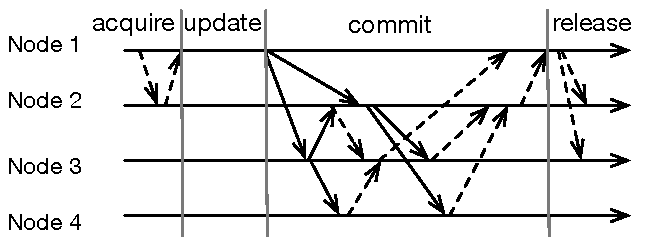
\includegraphics[width=\textwidth]{hotpot/Figures/mrsw.pdf}}
\caption[\mrsw\ Example.]
{
\mrsw\ Example.
Node 1 (\xn) first acquires write permission from Node 2 (\master)
before writing data.
It then commits the new data to \on{}s at Node 2 and 3 with replication degree four
and finally releases the write permission to \master.
}
\label{fig-mrsw}
\end{center}
\end{figure}
}


\subsection{MRSW Mode}
\label{sec:hotpot:mrsw}

The \mrsw\ mode allows only one writer to a \nvm\ page at a time
to trade parallelism for stronger consistency. 
%compared to the \mrmw\ mode.
\mrsw\ meets \ra, \rcm, and \re.

Traditional \mrsw\ protocols in DSM systems are usually invoked at every memory store
(\eg, to update cached read copies, to revoke current writer's write permission).
Unlike DSM systems, \dsnvm\ applications store and manage persistent data;
they do not need to ensure coherence on every memory store,
since they have well-defined points of when they want to start updating data and when they want to commit.
To avoid the cost of invoking coherence events on each memory store
while ensuring only one writer at a time, 
\hotpot\ uses an {\em \acquire} API for applications to indicate the data areas they want to update.
Afterwards, applications can update any date that they have acquired and use the \commitxact\ call to both 
commit updates and release corresponding data areas.
Figure~\ref{fig-mrsw} shows an example of \mrsw. % acquire, commit, and release process.

{\bf Acquire write permission.}
\hotpot\ uses a master node ({\em \master}) to maintain the active writer of each page. 
An \master\ can be one of the \hotpot\ node, the \cd, or a dedicated node.
%The \master\ maintains a simple hash table of the virtual page numbers of the data that is currently being written to.
When a node receives the \acquire\ call, it sends the virtual addresses of the data specified in the call to the \master.
If the \master\ finds that at least one of these addresses are currently being written to, 
it will reject the \acquire\ request and let the requesting node retry later.

{\bf Commit and release data.}
\mrsw's commit protocol is simpler and more efficient than \mrmw's,
since there is no concurrent commit operations to the same data in \mrsw\ (concurrent commit to different data pages is still allowed).
\mrsw\ combines phase 1 and phase 2 of the \mrmw\ commit protocol into a single phase 
where the \xn\ sends committing data to all \on{}s and all \on{}s commit data on their own.
%without the need to coordinate with other \on{}s.
Each \on\ individually handles commit in the same way as in the \mrmw\ mode, 
except that it does not need to coordinate with any other \on{}s or the \xn. 
\on\ directly proceeds to propagating data to \dn{}s after it has written its own redo log.

At the end of the commit process, the \xn\ informs the \on{}s to delete their redo logs (same as \mrmw\ commit phase 3)
and the \master\ to release the data pages.



\subsection{Crash Recovery}
\label{sec:hotpot:recovery}

\hotpot\ can safely recover from different crash scenarios
without losing applications' data.
% as long as the number of concurrent
%node failures is less than the application-specified replication degree.
\hotpot\ detects node failures
%by detecting an unresponsive node during a network operation and 
by request timeout 
and by periodically sending heartbeat messages from 
the \cd\ to all \hotpot\ nodes.
We now explain \hotpot's crash recovery mechanism
in the following four crash scenarios.
Table~\ref{tbl-crash} summarizes various crash scenarios and \hotpot's recovery mechanisms.

%\subsubsubsection{Crash During Transaction Commit}

{
\begin{table}[t]\small
\begin{center}
\begin{center}
\begin{tabular}{ p{0.18in} | p{0.5in} | p{0.25in} | p{0.5in} | p{4in} }
 & \small Node & \small \nvm & \small Time & \small Action \\
\hline
\hline
& any & Y & any & resume normal operation after reboot \\
\hline
& \cd\ & N & any & reconstruct using mirrored copy \\
\hline
& \on\ & N & NC & promote an existing \dn\ to \on\ \\
& \dn\ & N & NC & reconstruct data to meet replication degree \\
\hline
\multirow{7}{*}{\rotatebox{90}{\mrmw\ Commit}} & \xn/\on\ & N & p1 & undo commit, \on{}s delete redo logs \\
%& any & Y & any & continue commit \\
%& \on\ & N & p1 & undo commit, \on{}s delete redo logs \\
& \xn\ & N & p2 & redo commit, \on{}s send new data to \dn{}s \\
& \on\ & N & p2 & redo commit, \xn\ sends new data to new \on\ \\
& \dn\ & N & p2 & continue commit, \on\ sends data to new \dn\ \\
& \xn\ & N & p3 & complete commit, \on{}s delete redo logs \\
& \on/\dn\ & N & p3 & complete commit, new chunk reconstructed using \committed\ data \\
\hline
\multirow{5}{*}{\rotatebox{90}{MRSW}} & \xn\ & N & commit & undo commit, \on{}s send old data to \dn{}s \\
& \on\ & N & commit & \xn\ redo commit from scratch\\
& \xn\ & N & release & complete commit, release data \\
& \on/\dn\ & N & release & complete commit, new chunk reconstructed using \committed\ data \\
%& \xn\ & N &  & \\
%& \xn\ & N &  & \\
%\hline
\end{tabular}
\end{center}
\caption[Crash and Recovery Scenarios.]
{Crash and Recovery Scenarios.
Columns represent crashing node, if \nvm\ is accessible after crash, time of crash, and actions taken at recovery.
NC represents non-commit time.
}
\label{tbl-crash}
\end{center}
\end{table}
}


{\bf Recovering \cd\ and \master.}
\cd\ maintains node membership and dataset name mappings.
\hotpot\ currently uses one \cd\ but can be easily extended to 
include a hot stand-by \cd\ (\eg, using Mojim~\cite{Zhang15-Mojim}).
%When the primary \cd\ fails, the stand-by \cd\ can resume immediately.

\master\ tracks which node has acquired write access to a page under the \mrsw\ mode.
\hotpot\ does not make this information persistent
and simply reconstructs it by contacting all other nodes during recovery.
%If the \cd\ fails, a new node will be selected as \cd.
%Since all the metadata that the \cd\ maintains can be reconstructed, 
%\hotpot\ simply rebuild them by contacting all \hotpot\ nodes.

{\bf Non-commit time crashes.}
Recovering from node crashes during non-commit time is fairly straightforward.
If the \nvm\ in the crashed node is accessible after the crash (we call it {\em with-\nvm\ failure}),
\hotpot\ directly restarts the node and
lets applications access data in \nvm.
% provides the data in \nvm\ to applications,
%which can choose to resume from where they left over~\cite{Narayanan12-ASPLOS}.
As described in Section~\ref{sec:hotpot:singleconsistency}, \hotpot\ ensures crash consistency of a single node.
Thus, \hotpot\ can always recover to a consistent state 
when \nvm\ survives a crash.
\hotpot\ can sustain arbitrary number of with-\nvm\ failures concurrently. 

When a crash results in corrupted or inaccessible \nvm\ (we call it {\em no-\nvm\ failure}),
\hotpot\ will reconstruct the lost data using redundant copies.
\hotpot\ can sustain $N-1$ concurrent no-\nvm\ failures, where $N$ is the user-defined degree of replication.

If a \dn\ chunk is lost, 
the \on\ of this chunk will check what data pages in the chunk
have dropped below user-defined replication degree
and replicating them on the new node that replaces the failed node. 
%If a node fails and loses all its \dn{} data, and \hotpot\ 
%no longer meets the degree of replication requested by an application,
%the \on\ will send a committed copy of the failed node's data to the new node.
There is no need to reconstruct the rest of the \dn\ data;
\hotpot\ simply lets the new node access them on demand.

%\noindent{\bf Reconstructing \on{} chunks.}
When an \on\ chunk is lost, it is critical to reconstruct it quickly,
since an \on\ serves both remote data read and 
commit operations.
%If a node fails and loses its \on\ chunks,
Instead of reconstructing a failed \on\ chunk from scratch,
\hotpot\ promotes an existing \dn\ chunk to an \on\ chunk
and creates a new \dn\ chunk.
%To promote a \dn\ chunk to an \on\ chunk,
%the newly promoted \dn\ will communicate with all the other \dn{}s of this chunk.
The new \on\ will fetch locally-missing committed data from other nodes
and reconstruct \on\ metadata for the chunk.
Our evaluation results show that it takes at most 2.3 seconds to promote
a 1GB \dn\ chunks to \on.

%\subsubsection{}
{\bf Crash during commit.}
If a with-\nvm\ failure happens during a \commitxact\ call,
\hotpot\ will just continue its commit process after restart.
When a no-\nvm\ failure happens during commit,
\hotpot\ takes different actions to recover depending on when the failure happens.

For \mrmw\ commit, if no-\nvm\ failure happens before all the \on{}s have created the persistent redo logs (\ie, before starting phase 2),
\hotpot\ will undo the commit and revert to the old committed state
by deleting the redo logs at \on{}s.
If a no-\nvm\ failure happens after all \on{}s have written the committing data to their persistent redo logs (\ie, after commit phase 1),
\hotpot\ will redo the commit by replaying redo logs.

For \mrsw, since we combine \mrmw's phase 1 and phase 2 into one commit phase,
%do not allow each \on\ to proceed with pushing updates to \dn{}s right after it has written its own persistent redo log,
we will not be able to tell whether or not an \on\ has pushed the committing data to \dn{}s 
when this \on\ experience a no-\nvm\ failure.
In this case, \hotpot\ will let \xn\ redo the commit from scratch. 
Even if the crashed \on\ has pushed updates to some \dn{}s,
the system is still correct after \xn\ redo the commit;
it will just have more \redundant\ copies.
When the \xn\ fails during \mrsw\ commit, \hotpot\ will undo the commit
by letting all \on{}s delete their redo logs and send old data to \dn{}s to overwrite \dn{}s' updated data.
%During this recovery process, \hotpot\ needs to know what are the \on{}s that are involved in the commit.
%Instead of contacting all nodes to discover which ones are the \on{}s,
%\hotpot\ uses the \master\ %to reduce the overhead of contacting all nodes
%to only contact the nodes that owns pages that have been acquired by the failed \xn.

During commit, \hotpot\ only supports either \xn\ no-\nvm\ failure or \on\ no-\nvm\ failure.
We choose not to support concurrent \xn\ and \on\ no-\nvm\ failures during commit,
because doing so largely simplifies \hotpot's commit protocol and improves its performance.
\hotpot's commit process is fast (under 250\mus\ with up to 16 nodes, see Section~\ref{sec:hotpot:results}).
Thus, the chance of \xn\ and \on\ both fail and lose their \nvm\ during commit is very small.
\hotpot\ always supports \dn\ no-\nvm\ failures during commit regardless of whether there are concurrent \xn\ or \on\ failure.


\section{Network Layer}
\label{sec:hotpot:network}

The networking delay in \dsnvm\ systems is crucial to their overall performance.
We implement \hotpot's network communication using RDMA. %(Remote Direct Memory Access), 
RDMA provides low-latency, high-bandwidth direct remote memory accesses with low CPU utilization.
\hotpot's network layer is based on LITE~\cite{lite-sosp17}, an efficient RDMA software stack we
built in the Linux kernel on top of the RDMA native APIs, {\em Verbs}~\cite{ibverbs}.

Most of \hotpot's network communication is in the form of RPC. % uses this RPC interface to implement most of its functionality. 
We implemented a customized RPC-like interface in our RDMA layer based on the two-sided RDMA send and receive semantics.
We further built a multicast RPC interface where one node can send a request to multiple nodes in parallel and let them each 
perform their processing functions and reply with the return values to the sending node.
Similar to the findings from recent works~\cite{FaSST}, two-sided RDMA works better and is more flexible 
for these RPC-like interfaces than one-sided RDMA. 

To increase network bandwidth, our RDMA layer enables multiple connections between each pair of nodes. 
It uses only one busy polling thread per node to poll a shared ring buffer for all connections, 
which delivers low-latency performance while keeping CPU utilization low.
Our customized RDMA layer achieves an average latency of 7.9\us\ to perform a \hotpot\ remote page read. %an RPC of 8B outgoing and 4KB incoming message size (equivalent to a remote page read).
In comparison, IPoIB, a standard IP layer on top of Verbs, requires 77\us\ for a round trip with the same size.




\if 0 
%Our \ib\ layer provides a richer and more efficient abstraction of \ib\ operations than 
%existing kernel-level \ib\ layers such as IPoIB and RDS.
To provide low-latency network performance for \hotpot, 
we made several unique design and implementation decisions that are different from previous 
\ib- and RDMA-based network implementations~\cite{Dragojevic14-NSDI,Nelson15-ATC,Kalia14-SIGCOMM}.
%IB-Verbs requires the application to post send (receive) requests to send (receive) queues.
%It uses completion messages in the completion queue to indicate the completion of requests 
%and supports both polling and interrupts to detect completions.
%IB-Verbs offers native IB performance and outperforms alternative IB protocols such as IPoIB and RDS.

%uses a thin protocol based on the reliable transportation mode of IB-Verbs. 

The basic primitive of our \ib\ layer is a pair of send and reply messages
between two nodes. 
With this primitive, one node sends a message to a remote node,
usually a request for an operation, and then waits for a reply.
After the remote node handles this request, it sends a reply back to the calling node,
finishing a send-reply round. 

Interestingly, although \ib's one-sided RDMA operations allow direct read and write to remote memory 
without involving remote side's CPU~\cite{Dragojevic14-NSDI}, 
using them to implement \hotpot\ incurs higher latency than RDMA send and receive~\cite{Kalia14-SIGCOMM}.
This is because one-sided RDMA is mainly useful when accessing remote memory without any states managed by remote side.
\hotpot\ maintains various states and metadata at each node. 
%These metadata need to be consistently updated with their data.
%For example, when a \dn\ accesses a remote page, 
%\hotpot\ uses the send-reply primitive to send a request to the \on. 
%The \on\ updates its list of \dn{}s with committed data copies
%and then sends the page back to the \dn.
Implementing complex \hotpot\ operations using one-sided RDMA requires the combination of several RDMA commands.
Even though the latency of one send or reply is slightly higher than a single one-sided RDMA command,
using send-reply to implement \hotpot\ operations achieves better performance than using one-sided RDMA.

On top of the send-reply primitive, our \ib\ layer further provides an efficient implementation of 
two new interfaces:
atomically sending a group of messages and waiting for reply, 
and multicasting send messages to a set of nodes and waiting for all replies from them.
Both these operations are useful in implementing \hotpot's transaction system.

Our \ib\ layer implements a persistent, append-only log in \nvm\ for receiving messages.
with the help of the Linux kernel slab allocator.
The slab allocator performs object-based allocation efficiently 
by maintaining lists of free objects 
where it allocates new objects from and frees objects into.
%Thus, the slab allocator has v
%The slab allocator is more efficient than 
%Instead of preallocating and maintaining a circular log,
The \ib\ layer allocates new receiving buffers in \nvm\ using the slab allocator
and provides an interface to free these buffers back to the slab lists.
%The \ib\ layer supports atomic operations 
%in \nvm\ and provides a free let .
\hotpot\ uses this mechanism to maintain a persistent redo log for transactions.
\hotpot\ only frees buffers in this log after a transaction has been committed.
\fi

\section{Applications and Evaluation}
\label{sec:hotpot:app}

This section presents the performance evaluation of two applications and a set of microbenchmarks.
We ran all experiments on a cluster of 17 machines, each with two Intel Xeon CPU E5-2620 2.40GHz
processors, 128 GB DRAM, and one 40 Gbps Mellanox ConnectX-3 InfiniBand network adapter;
a Mellanox 40 Gbps InfiniBand switch connects all of the machines. 
All machines run the CentOS 7.1 distribution and the 3.11.1 Linux kernel.

The focus of our evaluation is to understand the performance of \dsnvm's distributed memory model,
its commit protocols, and its data persistence cost. As there is no real \nvm\ in production yet,
we use DRAM as stand-in for \nvm. A previous study~\cite{Zhang15-NVMMStudy} shows that even though
\nvm\ and DRAM can have some performance difference, the difference is small and has much lower impact
on application performance than the cost of flushing data from CPU caches to \nvm, which we have
included in \hotpot\ and can measure accurately.

\subsection{Systems in Comparison}
\label{sec:hotpot:comparesys}
We compare \hotpot\ with one in-memory file system, two \nvm-based file systems, 
one replicated \nvm-based system, and three distributed shared memory systems.
Below we briefly describe these systems in comparison.

\noindent{\textbf{Single-Node File Systems.}} 
Tmpfs is a Linux file system that stores all data in main memory and does not perform any I/Os to storage devices.
\pmfs~\cite{Dulloor14-EuroSys} is a file system designed for \nvm. 
The key difference between \pmfs\ and a conventional file system is that its implementation of
\mmap\ maps the physical \nvm\ pages directly into the applications' address spaces rather than moving them back and
forth between the file store and the buffer cache.
\pmfs\ ensures data persistence using \sfence\ and \clflush\ instructions.

\noindent{\textbf{Distributed \nvm-Based Systems}}
Octopus~\cite{Octopus} is a user-level RDMA-based distributed file system designed for \nvm.
\Octopus\ provides a set of customized file APIs including read and write,
but does not support memory-mapped I/Os or provide data reliability and availability.
%Octopus data servers access local PM without stacking a local file system layer. In Octopus,
%files are distributed to data servers in a hash-based way.

Mojim~\cite{Zhang15-Mojim} is our previous work that uses a primary-backup model to replicate \nvm\ data
over a customized IB layer.
Similar to \hotpot, \pmfs, and Octopus, Mojim maps \nvm\ pages directly into application virtual memory address spaces.
Mojim supports application reads and writes on the primary node but only reads on backup nodes. 

\noindent\textbf{Distributed Shared Memory Systems.} 
We implemented two kernel-level DSM systems, {\em \dsmxact} and {\em \dsmnoxact}, on top of the same network stack as \hotpot's.
Both of them support multiple readers and single writer (MRSW)
and use a home node for each memory page to serve remote read and to store which nodes are the current readers and writer of the page, 
similar to HLRC~\cite{Li89-ACM,HLRC}.
We open source both these DSM systems together with \hotpot.

{
\begin{figure*}[th]\normalsize
\begin{minipage}{3.2in}
\begin{center}
\begin{tabular}{ c | c | c | c | c | c }\normalsize
\normalsize Workload & \normalsize Read & \normalsize Update & \normalsize Scan & \normalsize Insert & \normalsize R\&U \\
\hline
A & 50\% & 50\% & - & - & - \\
B & 95\% & 5\% & - & - & - \\
C & 100\% & - & - & - & - \\
D & 95\% & - & - & 5\% & - \\
E & - & - & 95\% & 5\% & - \\
F & 50\% & - & - & - & 50\% \\
\end{tabular}
\end{center}
\vspace{-0.2in}
\mycaption{tbl-ycsb}{YCSB Workload Properties.}
{
The percentage of operations in each YCSB workload. 
R\&U stands for Read and Update.
}
\end{minipage}
\begin{minipage}{0.05in}
\hspace{0.05in}
\end{minipage}
\begin{minipage}{3.6in}
\begin{center}
\centerline{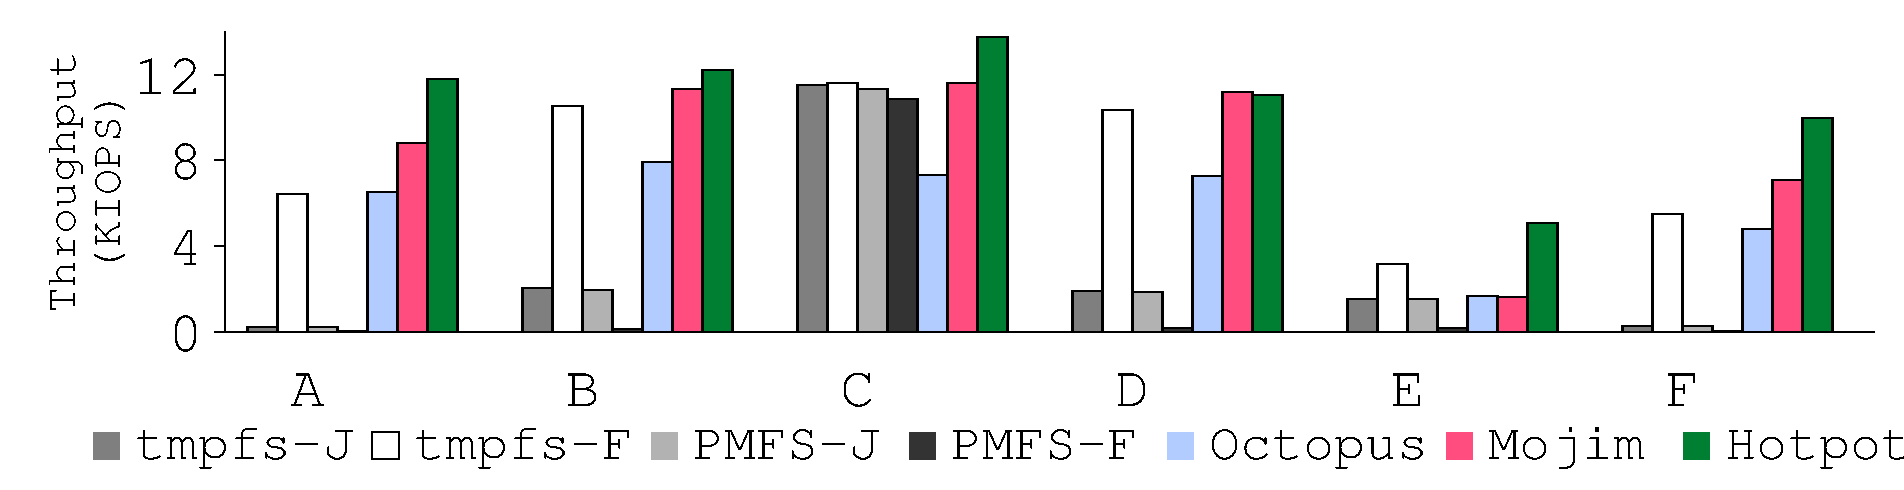
\includegraphics[width=3.8in]{Figures/g_plot_YCSB_run_throughput.pdf}}
\mycaption{fig-ycsbrun}{YCSB Workloads Throughput.}
{
}
\end{center}
\end{minipage}
\vspace{-0.2in}
\end{figure*}
}


\dsmxact\ guarantees release consistency using a transaction interface that is similar to \hotpot's \mrsw\ mode. 
Applications first call a transaction begin API to specify the data that they want to write.
Transaction begin only succeeds if no other writer is writing to any of the transaction data.
After beginning a transaction, applications can read and write to any transaction data
and use a transaction commit call to end a transaction. 
When committing a transaction, \dsmxact\ writes all updated transaction data to the home node, 
invalidates the read caches on all other nodes, 
and releases the write permission.

\dsmnoxact\ supports write (memory stores) without transactions and 
does not require applications to declare which data they want to write in advance.
On each write (memory store), \dsmnoxact\ revokes the write permission from the current writer, 
writes the current dirty data to the home node, and grants the write permission to the new writer.
Compared to \dsmxact, \dsmnoxact\ supports stronger consistency, requires less programmer efforts, 
but incurs higher performance overhead because of its more frequent writer invalidation.

Apart from the two DSM systems that we built, 
we also compare \hotpot\ with Grappa~\cite{Nelson15-ATC}, 
a recent DSM system that supports modern data-parallel applications. 
Different from traditional DSM systems and our DSM systems, Grappa moves computation to data instead of fetching data to where computation is.


\subsection{In-Memory NoSQL Database}
\label{sec:hotpot:mongodb}
MongoDB~\cite{MongoDB} is a popular distributed NoSQL database that supports several different storage engines
including its own storage engine that is based on memory-mapped files (called MMAPv1).
Applications like MongoDB can largely benefit from having a fast means to store and access persistent data. 
We ported MongoDB v2.7.0 to \hotpot\ by modifying its storage engine to keep track of all writes to the memory-mapped data file.
We then group the written memory regions belonging to the same client request into a \hotpot\ \commit\ call.
In total, porting MongoDB to \hotpot\ requires modifying 120 lines of code. 

To use the ported MongoDB, administrators can simply configure several machines to share 
a \dsnvm\ space under \hotpot\ and run ported MongoDB on each machine.
Applications on top of the ported MongoDB can issue requests to any machine, 
since all machines access the same \dsnvm\ space.
In our experiments, we ran the ported MongoDB on three \hotpot\ nodes
and set data replication degree to three.

We compare this ported MongoDB with the default MongoDB running on \tmpfs, \pmfs, and \Octopus, 
and a ported MongoDB to \Mojim\ on three nodes connected with IB.
Because \Octopus\ does not memory-mapped operations and MongoDB's storage engine is based on memory-mapped files,
MongoDB cannot directly run on \Octopus.
We run MongoDB on top of FUSE~\cite{fuse-fs}, a full-fledged user-level file system, 
which in turn runs on \Octopus.

%All these systems have three replicas of all data.
%\tmpfs, \pmfs, and \Octopus\ use MongoDB's default replication mechanism, 
For \tmpfs\ and \pmfs, we use two consistency models (called MongoDB write concerns):
the \journaled\ write concern and the \fsyncsafe\ write concern. With the \journaled\ write concern, MongoDB
logs data in a journal file and checkpoints the data in a lazy fashion. MongoDB blocks a client call until the
updated data is written to the journal file. With \fsyncsafe, MongoDB does not perform journaling. Instead, it flushes
all the dirty pages to the data file after each write operation and blocks the client call until this operation completes.
We run \Octopus\ and \Mojim\ with the \fsyncsafe\ write concern.
\Octopus, \tmpfs, and \pmfs\ provide no replication,
while \Mojim\ and \hotpot\ use their own replication mechanisms to make three replicas of all data 
(\Mojim\ uses one node as the primary node and the other two nodes as backup nodes).

\if 0
We first evaluate a simple microbenchmark that inserts key-value pairs to MongoDB. 
Each insert operation contains 10 key-value pairs, with each pair containing 100 bytes of randomly generated data.
Figure~\ref{fig-ycsbload} presents the average latency (in log scale) of key-value pair insertions. 
MongoDB on \hotpot\ outperforms the both write concerns on \pmfs.
\pmfs\ performs worse mainly because of its file system layer software overhead 
and inefficient process of making data persistent.
%uses a more efficient network layer. 
%\journaled\ write concern needs to make journal persistent
%and \fsyncsafe\ write concern makes the whole data file persistent at every write.
%This performance gain is mainly due to \hotpot's efficient replication protocol and networking stack.
\fi


{
\begin{figure*}[th]
\begin{center}
\centerline{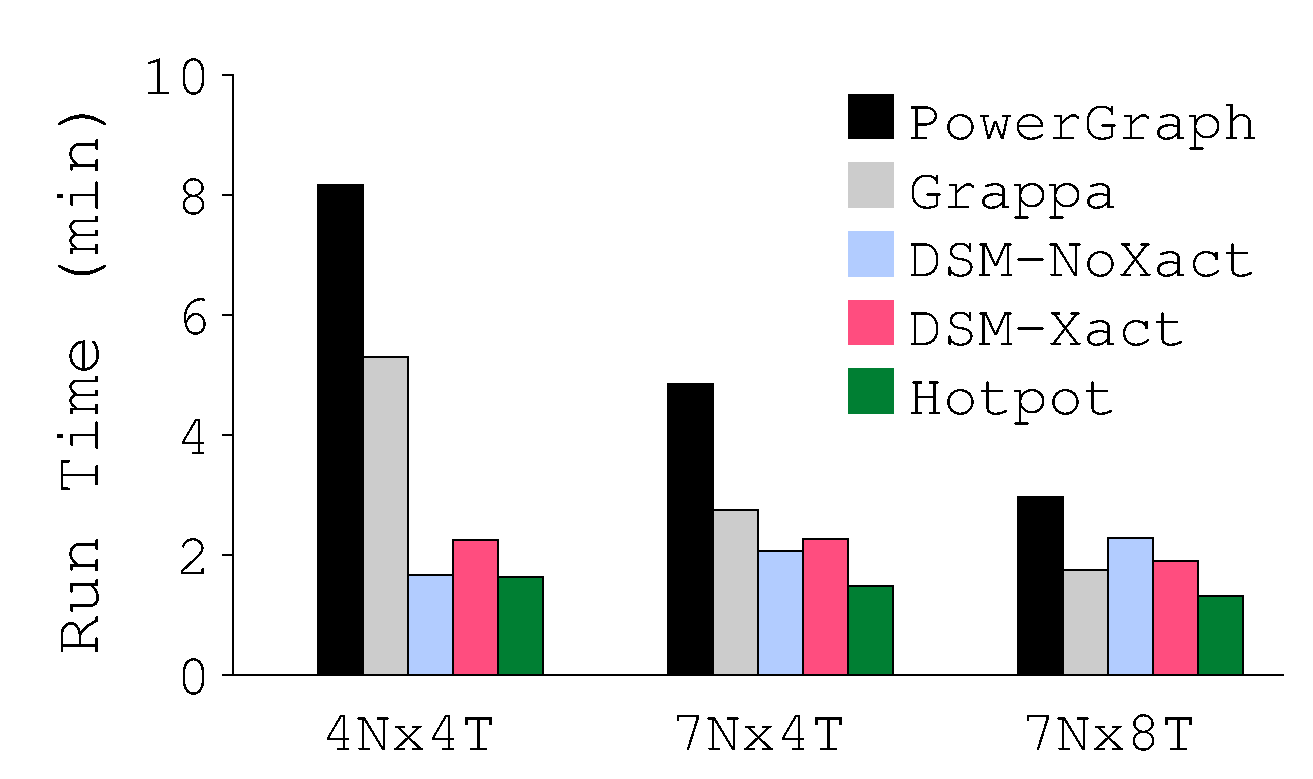
\includegraphics[width=0.6\textwidth]{hotpot/Figures/g_plot_graph_ATC_runtime.pdf}}
\caption[Pagerank Total Run Time.]
{
Pagerank Total Run Time.
N stands for total number of nodes, T stands for number of threads running on a node.
}
\label{fig-graph-runtime}
\end{center}
\end{figure*}
}
{
\begin{figure*}[th]
\begin{center}
\centerline{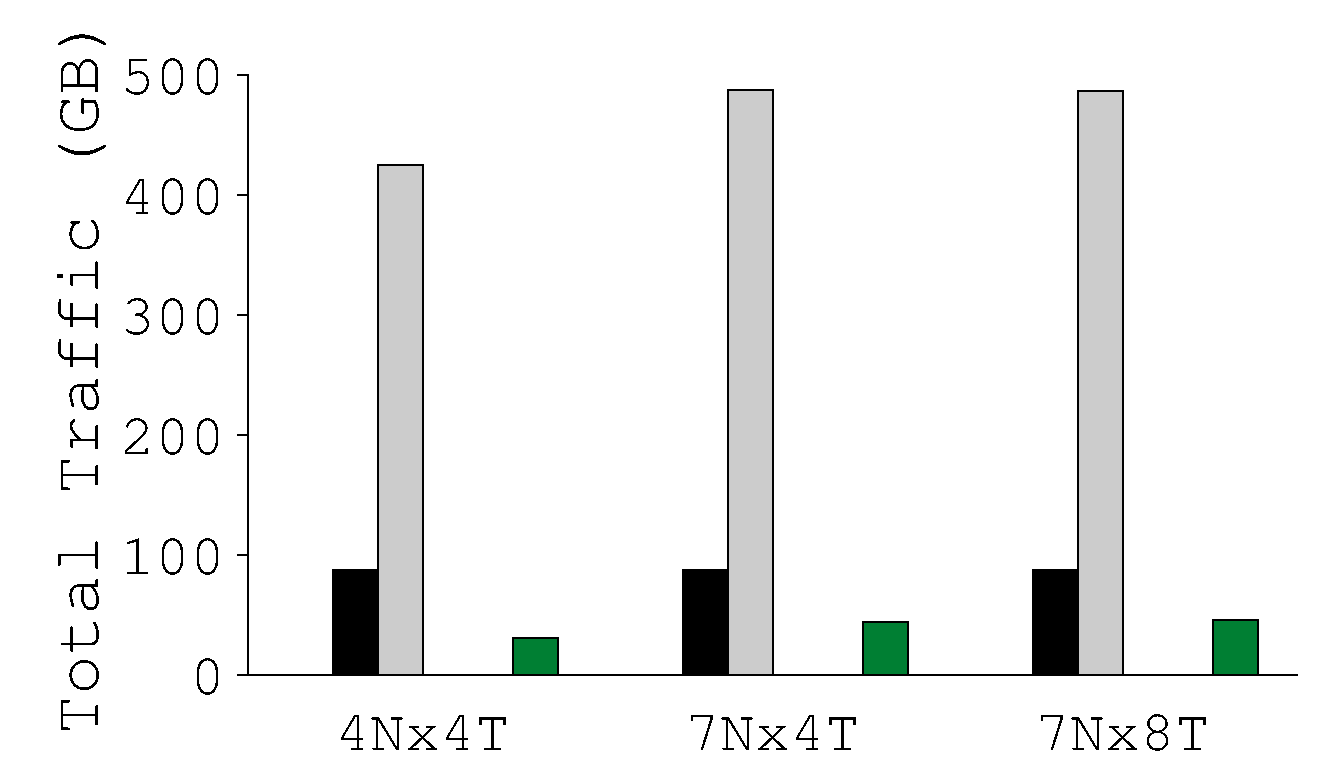
\includegraphics[width=0.6\textwidth]{hotpot/Figures/g_plot_graph_ATC_network.pdf}}
\caption[Pagerank Total Network Traffic.]
{
Pagerank Total Network Traffic.
}
\label{fig-graph-traffic}
\end{center}
\end{figure*}
}
{
\begin{figure*}[th]
\begin{center}
\centerline{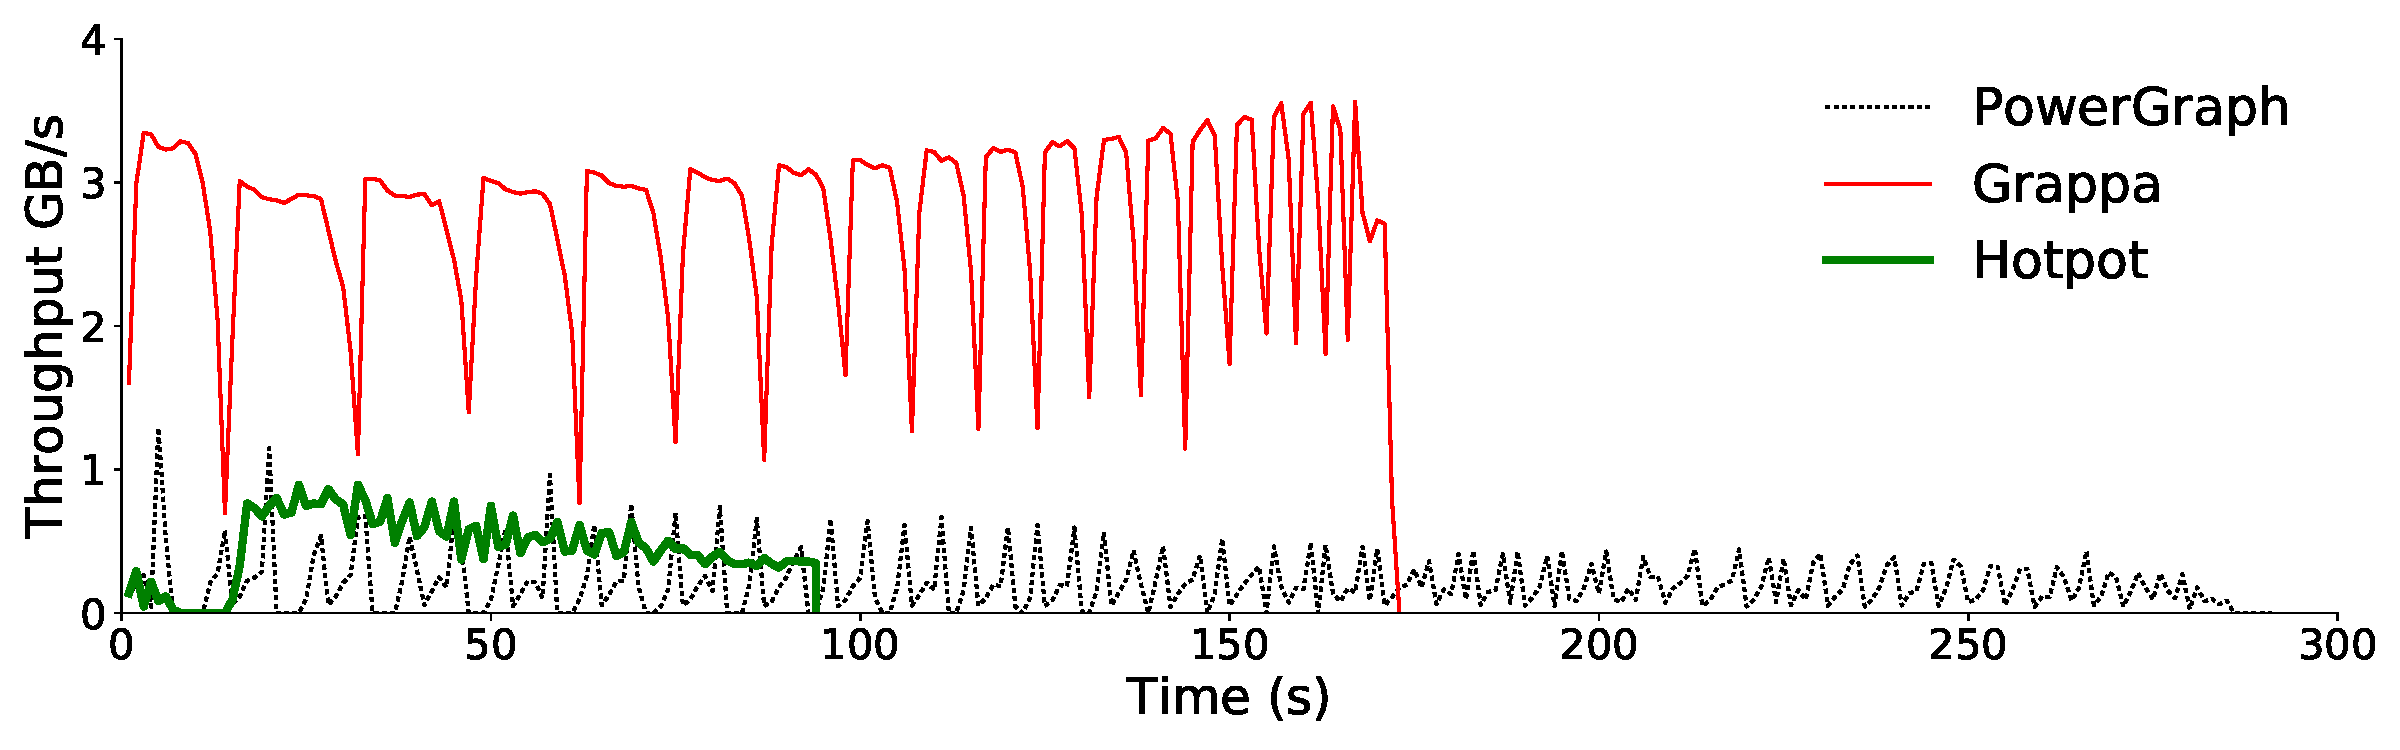
\includegraphics[width=\textwidth]{hotpot/Figures/g_plot_combined_trace_timewindow.pdf}}
\caption[Pagerank Network Traffic Over Time.]{Pagerank Network Traffic Over Time.}
\label{fig-graph-timeline}
\end{center}
\end{figure*}
}


YCSB~\cite{Cooper10-CloudCom} is a key-value store benchmark 
that imitates web applications' data access models. 
Figure~\ref{tbl-ycsb} summarizes the number of different operations in the YCSB workloads.
Each workload performs 10,000 operations on a database with 100,000 1\KB\ records.
Figure~\ref{fig-ycsbrun} presents the throughput of MongoDB on \tmpfs, \pmfs, Octopus, Mojim, and \hotpot\ using YCSB workloads. 

For all workloads, \hotpot\ outperforms \tmpfs, \pmfs, \Octopus, and \Mojim\ for both the \journaled\ and the \fsyncsafe\ write concerns. 
The performance improvement is especially high for write-heavy workloads.
\pmfs\ performs worst mainly because of its inefficient process of making data persistent with default MongoDB.
The default MongoDB \fsync{}s the whole data file after each write under \fsyncsafe,
and \pmfs\ flushes all cache lines of the file to \nvm\ by performing one \clflush\ at a time.
\hotpot\ and Mojim only commit dirty data, largely improving MongoDB performance over \pmfs.
Compared to \tmpfs\ and \pmfs\ under \journaled, \hotpot\ and Mojim use their own mechanisms to 
ensure data reliability and avoid the performance cost of journaling.
Moreover, \hotpot\ and Mojim make three persistent replica for all data, while \pmfs\ makes only one.
Tmpfs is slower than \hotpot\ even though \tmpfs\ does not make any data persistent, 
because MongoDB's slower replication mechanism on IPoIB.
\hotpot's network layer is significantly better than IPoIB~\cite{lite-sosp17}.

\Octopus\ performs worse than \hotpot\ and \Mojim\ because it incurs significant overhead of additional {\em indirection layers}:
each memory operation within the memory-mapped file goes through the FUSE file system and then through \Octopus.
\hotpot\ and \Mojim\ both support native memory instructions and incurs no indirection overhead.
Finally, even though Mojim's replication protocol is simpler and faster than \hotpot's,
\hotpot\ outperforms Mojim because Mojim only supports write on one node while \hotpot\ supports write on all nodes.

\subsection{Distributed (Persistent) Graph}
Graph processing is an increasingly important type of applications in modern 
datacenters~\cite{Gonzalez12-OSDI,Gonzalez14-OSDI,Kyrola12-OSDI,Low10-UAI,Low12-VLDB,Malewicz10-SIGMOD}.
Most graph systems require large memory to run big graphs.
Running graph algorithms on \nvm\ not only enables them to exploit the big memory space the high-density \nvm\ provides,
but can also enable graph algorithms to stop and resume in the middle of a long run.

We implemented a distributed graph processing engine on top of \hotpot\ based on the PowerGraph design~\cite{Gonzalez12-OSDI}.
It stores graphs with vertex-centric representation in \dsnvm\ with random order of vertices
and distributes graph processing load to multiple threads across all \hotpot\ nodes.
Each thread performs graph algorithms on a set of vertices in three steps: gather, apply, and scatter, 
with the optimization of delta caching~\cite{Gonzalez12-OSDI}.
After each step, we perform a global synchronization with \barrier\ and only start the next step when all threads have finished the last step.
At the scatter step, the graph engine uses \hotpot's \mrsw\ \commitxact\ to make local changes of the scatter values 
visible to all nodes in the system. We implemented the \hotpot\ graph engine with only around 700 lines of code.
Similarly, we implemented two distributed graph engines on top of \dsmxact\ and \dsmnoxact;
these engines differ from \hotpot's graph engine only in the way they perform data write and commit.

We compare \hotpot's graph engine with \dsmxact, \dsmnoxact, PowerGraph, and Grappa~\cite{Nelson15-ATC} with two real datasets,
Twitter (41\,M vertices, 1\,B directed edges)~\cite{Kwak10-WWW} and LiveJournal (4\,M vertices, 34.7\,M undirected edges)~\cite{snapnets}.
For space reason, we only present the results of the Twitter graph, but the results of LiveJournal are similar.
Figure~\ref{fig-graph-runtime} shows the total run time of the PageRank~\cite{PageRank} algorithm with
\hotpot, \dsmxact, \dsmnoxact, PowerGraph, and Grappa under three system settings:
four nodes each running four graph threads, seven nodes each running four threads, and seven nodes each running eight threads.

\hotpot\ outperforms PowerGraph by 2.3\x\ to 5\x\ and Grappa by 1.3\x\ to 3.2\x.
In addition, \hotpot\ makes all intermediate results of graph persistent for fast restart. 
A major reason why \hotpot\ outperforms PowerGraph and Grappa even when \hotpot\
requires data persistence and replication is \hotpot's network stack.
Compare to the IPoIB used in PowerGraph and Grappa's own network stack,
\hotpot's RDMA stack is more efficient.

Our implementation of \dsmxact\ and \dsmnoxact\ use the same network stack as \hotpot,
but \hotpot\ still outperforms \dsmnoxact\.
\dsmnoxact\ ensures cache coherence on every write and thus incurs much higher performance overhead than \hotpot\ and \dsmxact.

To further understand the performance differences, we traced the network traffic of these three systems.
Figure~\ref{fig-graph-traffic} plots the total amount of traffic %in the PageRank run for PowerGraph, Grappa, and \hotpot. 
and Figure~\ref{fig-graph-timeline} plots a detailed trace of network activity of the 7Nx4T setting.
\hotpot\ sends less total traffic and achieves higher bandwidth than PowerGraph and Grappa.

{
\begin{figure*}[th]
\begin{center}
\centerline{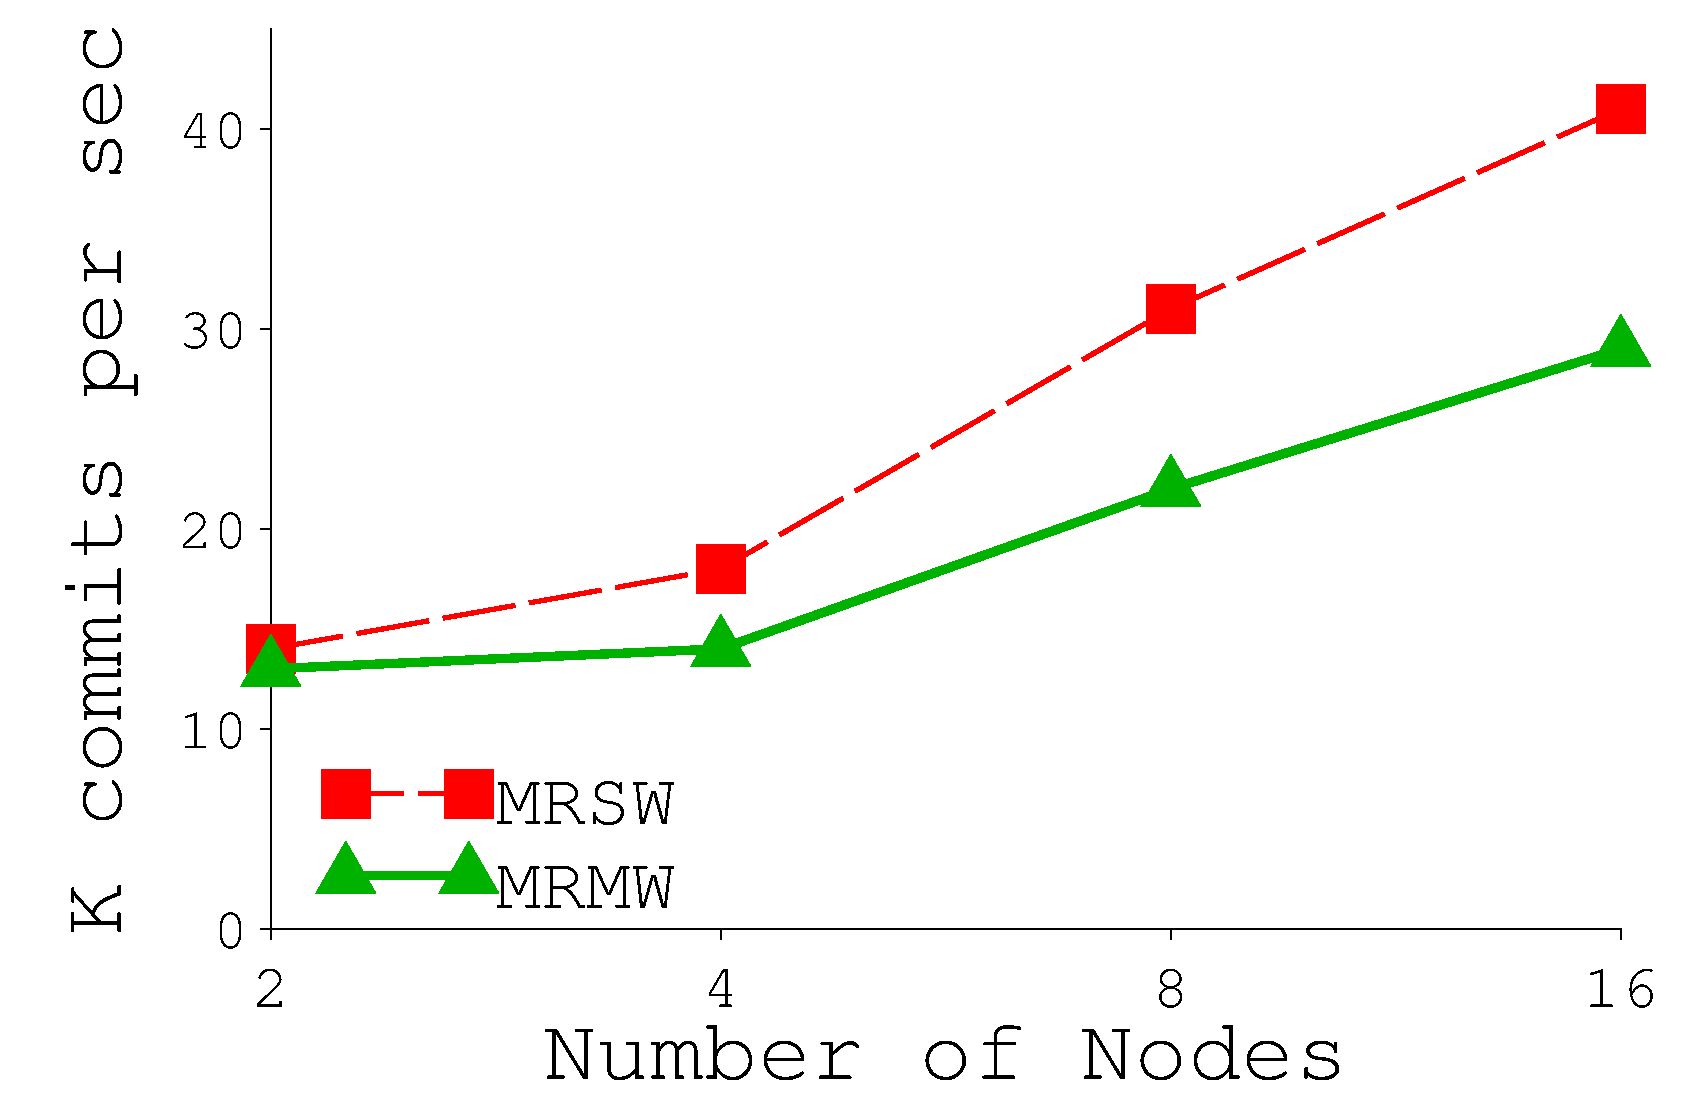
\includegraphics[width=0.6\textwidth]{hotpot/Figures/g_plot_SOCC_node.pdf}}
\caption[\hotpot\ Scalability.]
{
\hotpot\ Scalability.
Commit throughput with 2 to 16 nodes.
}
\label{fig-nodescale}
\end{center}
\end{figure*}
}
{
\begin{figure*}[h]
\begin{center}
\centerline{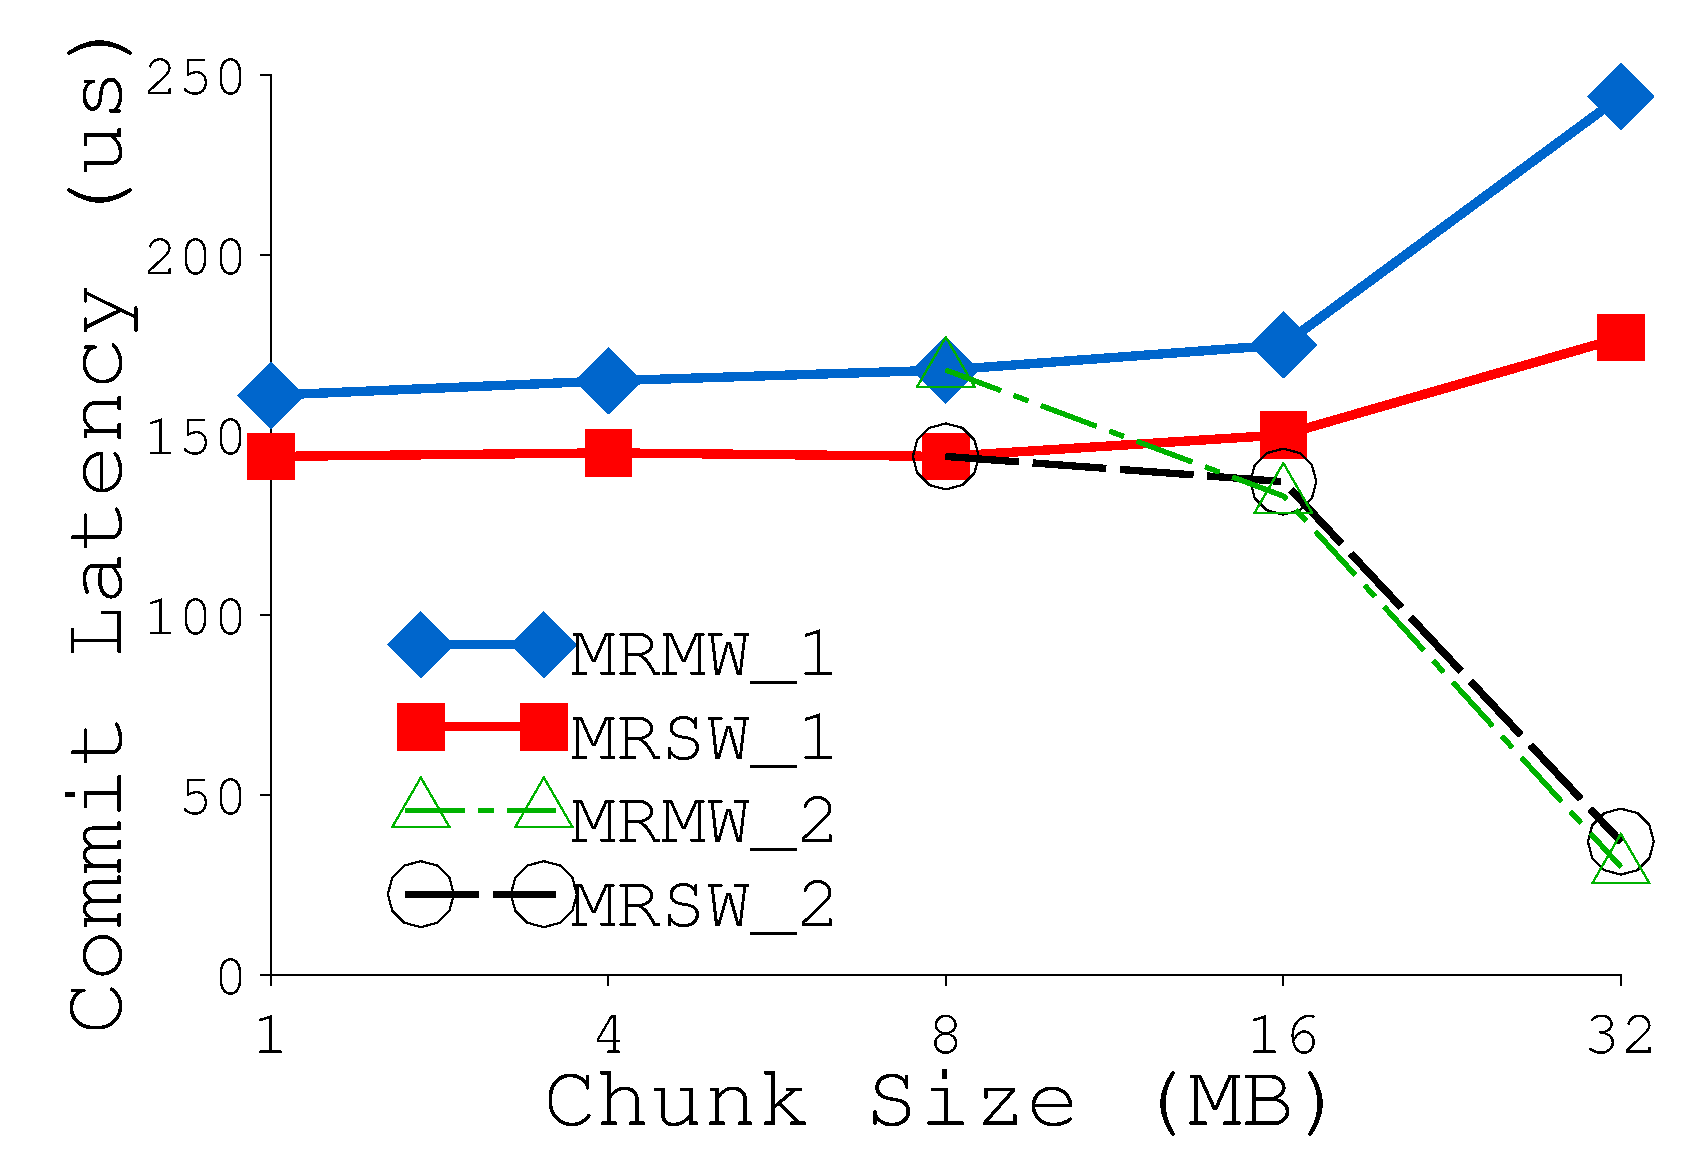
\includegraphics[width=0.6\textwidth]{hotpot/Figures/g_plot_SOCC_chunksize.pdf}}
\caption[Chunk Size.]
{
Chunk Size.
For 16\MB\ and 32\MB\ cases, 1 represents \on\ being remote and 2 represents \xn\ being \on. 
}
\label{fig-chunksize}
\end{center}
\end{figure*}
}
{
\begin{figure*}[h]
\begin{center}
\centerline{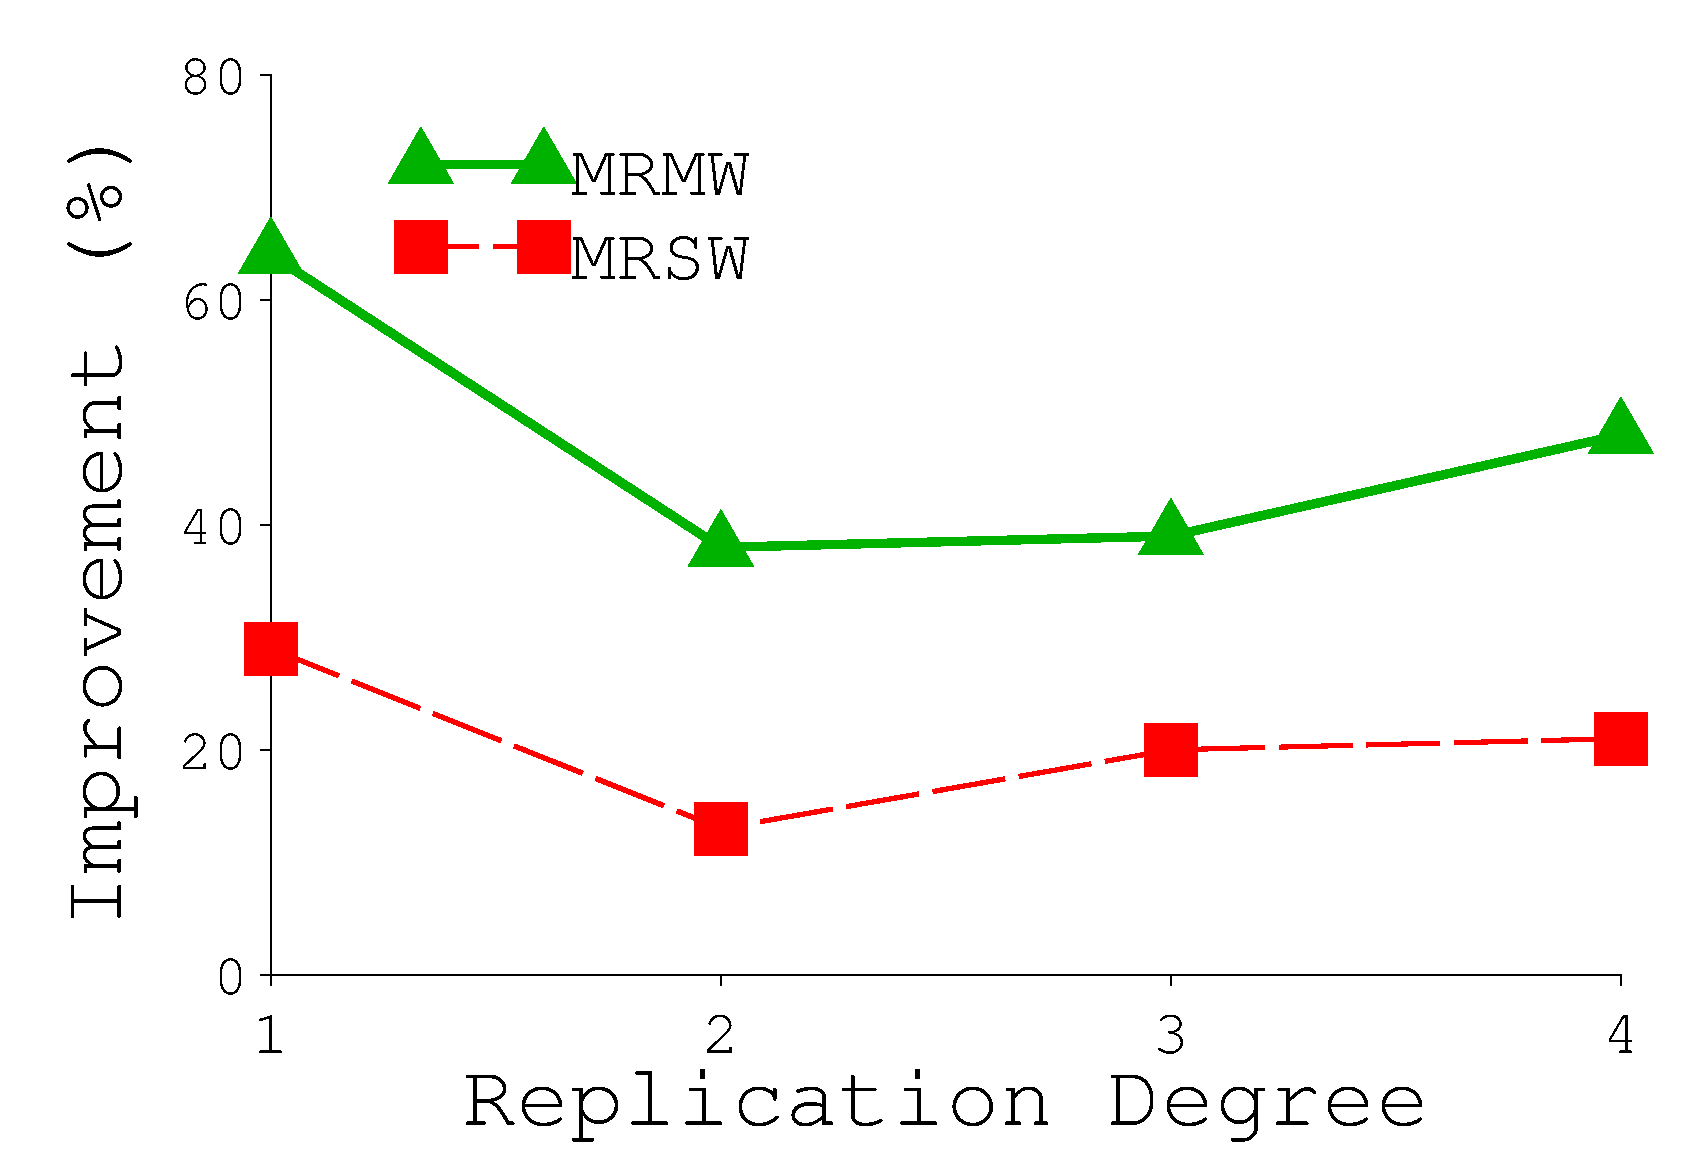
\includegraphics[width=0.6\textwidth]{hotpot/Figures/g_plot_SOCC_migration.pdf}}
\caption[\on\ Migration.]
{
\on\ Migration.
The improvement of average commit latency with \on\ migration over no migration.
}
\label{fig-migration}
\end{center}
\end{figure*}
}
{
\begin{figure*}[h]
\begin{center}
\centerline{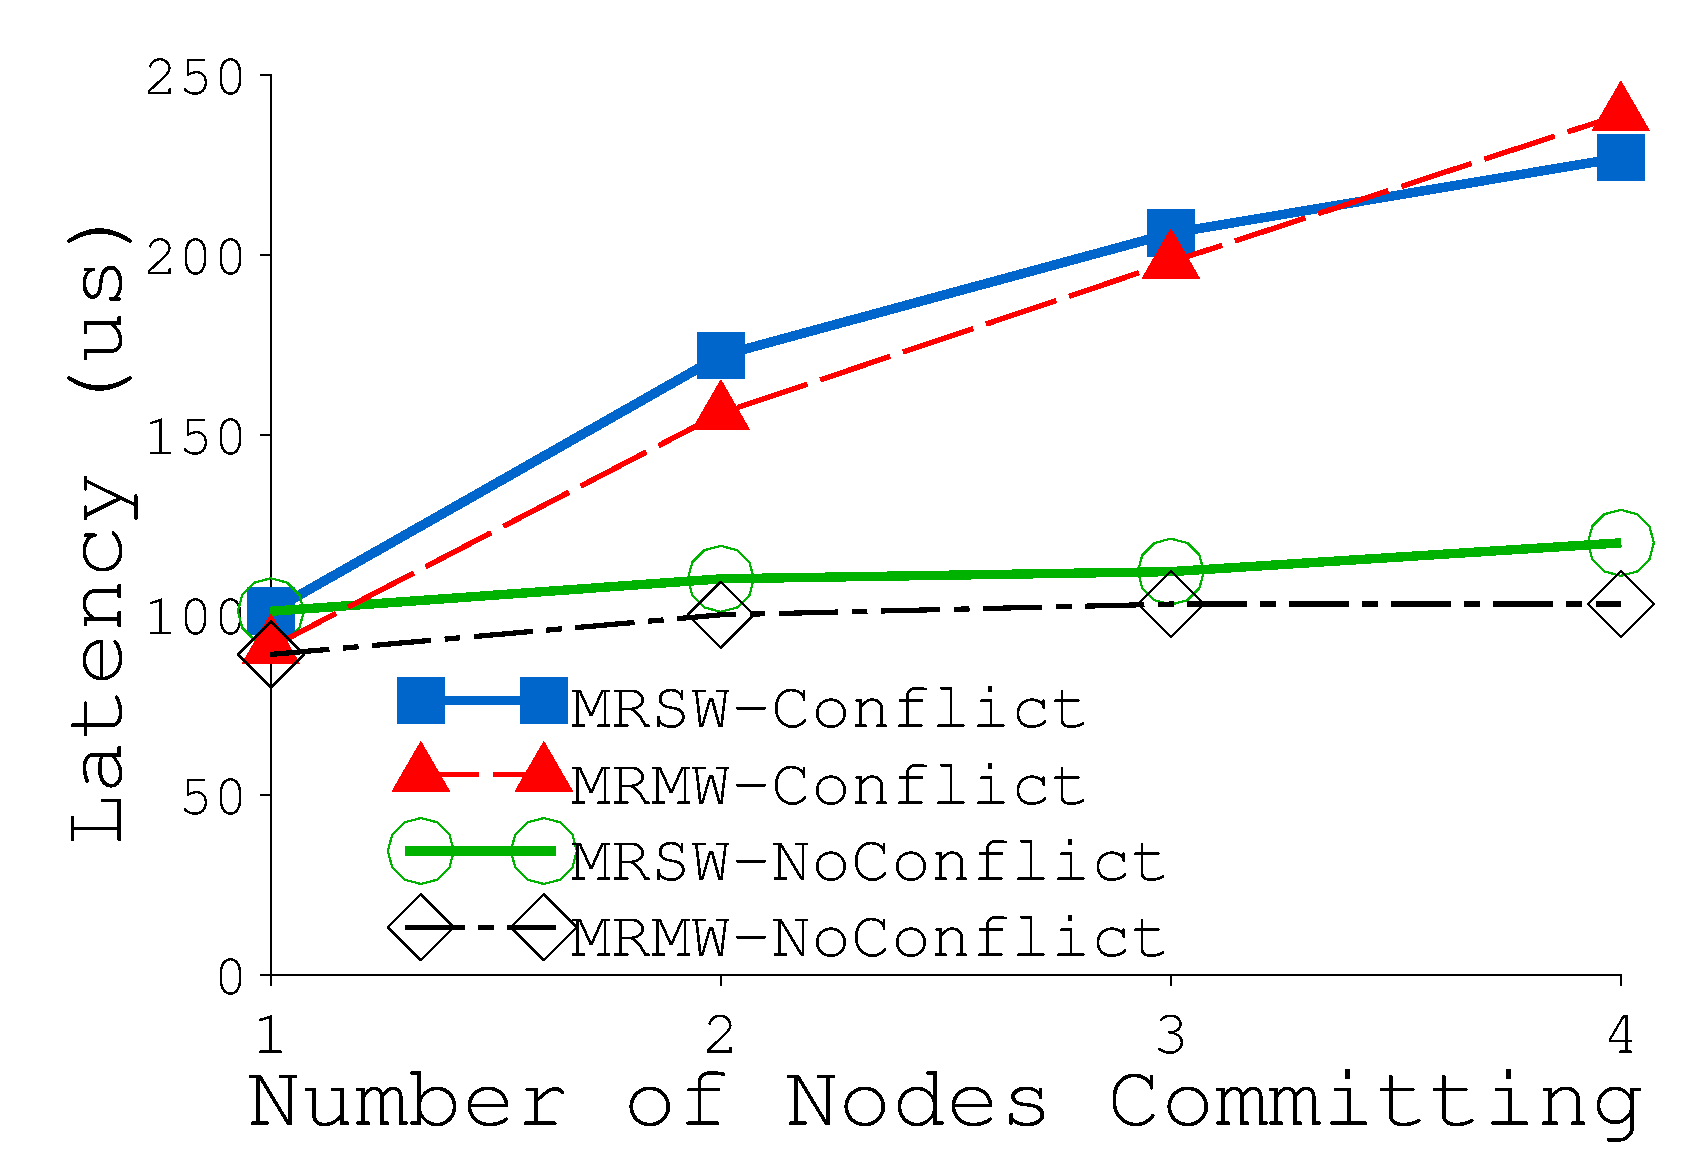
\includegraphics[width=0.6\textwidth]{hotpot/Figures/g_plot_SOCC_conflict.pdf}}
\caption[Commit Conflict.]
{
Commit Conflict.
Average commit latency with and without conflict.
}
\label{fig-conflict}
\end{center}
\end{figure*}
}
\subsection{Micro-Benchmark Results}
\label{sec:results}

We now present our microbenchmark results that evaluate the effect of different system settings and parameters.
Since \hotpot\ reads have a constant latency (around 7.9\us) and \hotpot\ writes do not go through network,
\hotpot's performance is largely affected by its data commit process.
Because of space reasons, we focus our microbenchmark experiments on commit.

\noindent{\bf Scalability.}
Figure \ref{fig-nodescale} shows the total commit throughput of \hotpot\ on 2 to 16 nodes with a workload 
that lets all nodes concurrently commit 32 random 4\KB\ areas with replication degree 1. 
Overall, both \mrmw\ and \mrsw\ commit scale.
As expected, \mrmw\ \commitxact\ is more costly than \mrsw. 

\noindent{\bf Replication degree and committing size.} 
%Figure \ref{fig-repdegree}
We next evaluate the effect of replication degree and the total amount of data in a \commitxact\ call.
%using a workload that let four nodes concurrently commit 32 sequential 4\KB\ areas. 
As expected, with higher replication degree and with more committing data, \commitxact\ takes longer for both \mrmw\ and \mrsw.
%since more replica needs to be made.
Because of space reasons, we do not include figures for these experiments.

\noindent{\bf Chunk size.}
We use a controlled microbenchmark to showcase the effect of chunk size (Figure~\ref{fig-chunksize}).
Each run has one node in a cluster of four nodes committing 32 1\KB\ areas that span a 32\MB\ region evenly with replication degree 1.
Since \hotpot\ distributes chunks in Round Robin, 
when chunk size is below 8\MB, the 32\MB\ region will be distributed equally to all four nodes.
The \commitxact\ performance stays similar with 1, 4, and 8\MB\ chunk size,
since \commitxact\ will always use all four nodes as \on{}s.
When chunk size is 16\MB\ (or 32\MB), only two (or one) nodes are \on.
We observe two different behaviors:
when the \xn\ happens to also be the \on\ of the chunk that contains the committing data,
the \commitxact\ performance is better than when chunk size is below 8\MB, since half (or all) commit happens locally at the \xn.
But when the \xn\ is not \on, all commit traffic goes to only two (or one) remote nodes,
resulting in worse performance than when chunk size is small.
This result suggest that smaller chunk size has better load balancing.

\noindent{\bf \on\ migration.}
From the previous experiments, we find that the \commitxact\ performance depends heavily on the location of \on\
and the initial \hotpot\ \on\ assignment may not be optimal.
We now evaluate how effective \hotpot's \on\ migration technique is in improving \commitxact\ performance (Figure~\ref{fig-migration}). 
We ran a workload with Zipf distribution to model temporal locality in datacenter applications~\cite{Atikoglu12,Breslau99} on four nodes with replication degree 1 to 4.
Each node issues 100,000 \commitxact\ calls to commit two locations generated by Zipf.
With \on\ migration, the \commitxact\ performance improves by 13\% to 29\% under \mrsw\ and 38\% to 64\% under \mrmw.
\on\ migration improves performance because the node that performs most \commitxact\ on a chunk becomes its \on\ after migration.
The improvement is most significant with replication degree one, 
because when \xn\ is \on\ and replication degree is one, there is no need to perform any network communication.
\mrmw's improvement is higher than \mrsw, because \mrmw\ can benefit more from committing data locally
--- the \mrmw\ commit process that involves remote \on{}s is more costly than that of \mrsw.

\noindent{\bf Effect of conflict commits.}
Figure~\ref{fig-conflict} compares the \commitxact\ performance of when 1 to 4 nodes in a four node cluster 
concurrently commit data in two scenarios:
all \xn{}s commit the same set of data (32 sequential 1\KB\ areas) at the same time which results in commit conflict,
%and synchronizes all nodes the commit at the same time, resulting in commit conflict.
and \xn{}s use different set of data without any conflict.
Commit conflict causes degraded performance, 
and the degradation is worse with more conflicting nodes.
However, conflict is rare in reality, since \commitxact\ is fast.
Conflict only happens when different nodes commit the same data page at exactly the same time.
In fact, we had to manually synchronize all nodes at every \commitxact\ call using \barrier\ to create conflict.

\section{Related Work}
\label{sec:related}

There have been a host of distributed shared memory systems and
distributed storage
systems~\cite{AdyaEtAl-Farsite,calder11-azure,DeCandia+07-Dynamo,Ghemawat03-GoogleFS,KubiEtAl00-Ocean,Petersen97-Bayou,Terry13-Pileus,Chun06-NSDI,Gibbons91-SPAA,Krieger90-HICSS,Zhang15-SOSP,Zhou92-IEEE,Stumm90-IEEE,Stumm90-IPDPS,HLRC,Shasta}
over the past few decades.
While some of \hotpot's coherence protocols may resemble existing DSM systems, none of them manages persistent data.
There are also many single-node \nvm\ systems~\cite{MemoryPersistency,pmxact-asplos16,Delegated-persist,sosp09:bpfs,Dragojevic14-NSDI,Dulloor14-EuroSys,Xiaojian11-SC,HiNFS-Eurosys16,Kamino-EuroSys17,Coburn11-ASPLOS,Volos11-ASPLOS},
but they do not support distributed environments.

\Octopus~\cite{Octopus} is a user-level RDMA-based distributed \nvm\ file system developed in parallel with \hotpot.
\Octopus\ manages file system metadata and data efficiently in a pool of PM-equipped machines. 
\Octopus\ provides a set of customized file APIs including read and write
but not any memory-mapped interfaces.
\Octopus\ does not provide data reliability and high availability either.
\hotpot's abstraction is memory based rather than file based,
and it offers data reliability, availability, and different consistency levels.

Grappa~\cite{Nelson15-ATC} is a DSM system that supports modern data-parallel applications.
Instead of fetching remote memory to a local cached copy, Grappa executes functions at the remote side.
\hotpot\ is a \dsnvm\ system and lets applications store persistent data.
It fetches remote data for both fast local access and data replication.

FaRM~\cite{Kalia14-SIGCOMM,Dragojevic14-NSDI} is an RDMA-based
distributed system on battery-backed DRAM.
RAMCloud is a low-latency distributed key-value store system that keeps a single copy of all data in DRAM~\cite{Ongaro11-RamCloud}
%While \hotpot\ and RAMCloud both provide reliable memory-based storage systems,
%RAMCloud provides a key-value interface to applications
and replicates data on massive slower storages for fast recovery.
%rather than a memory-like interface to applications.
The major difference between \hotpot\ and FaRM or RAMCloud is that
FaRM and RAMCloud both adds a software indirection layer for key-value stores
which can cause significant latency overhead over native load/store operations
and obscures much of the performance of the underlying \nvm.
\hotpot\ uses a memory-like abstraction and directly stores persistent data in \nvm.
\hotpot\ also performs data persistence and replication differently
and uses a different network layer based on two-sided RDMA.

Crail~\cite{crail} is an RDMA-based high-performance multi-tiered distributed storage system that integrates with the Apache Spark ecosystem~\cite{Zaharia12-NSDI}.
Crail mainly consists of a file system that manages tiered storage resources (\eg, DRAM, flash, disk) 
with flexible allocation policies across tiers.
\hotpot\ is a pure \nvm-based system that exposes a memory-like interface. 

PerDis~\cite{PerDis} and Larchant~\cite{Larchant,Larchant94} use a distributed file system below a DSM layer.
%, data management,
%data replication, and cache coherence, a set of challenges more demanding than these layered systems.
Unlike these systems, \hotpot\ is a single-layer system that provides shared memory access, data persistence, and reliability.
%Unlike Crail, \hotpot\ leverages PM to combine DRAM and persistent storage into one layer, and
%fulfills application's requirement at the same time.


\if 0
\textcolor{Red}
{
Pelly et al.~\cite{MemoryPersistency} proposes memory persistency, which defines
the ordering of persists to PM. Kolli et al.~\cite{pmxact-asplos16,Delegated-persist}
try to implement PM transactions more efficiently by reducing persist dependencies.
In \hotpot, consistency is either guaranteed by a single 8-byte failure-atomic write without logging or CoW,
or by local logging of distributed transactions.
}
\fi

Our own previous work, Mojim~\cite{Zhang15-Mojim}, provides an efficient mechanism to replicate \nvm\
over IB using a primary-backup protocol.
\hotpot\ is a \dsnvm\ system that provides a shared-memory abstraction
and integrates cache coherence and data replication.

\section{Conclusion}
\label{sec:conclude}

We presented \hotpot, a kernel-level DSPM system that provides applications
with a shared persistent memory abstraction. Our evaluation results show that
it is easy to port existing applications to Hotpot and the resulting systems
significantly outperform existing solutions.

\chapter{LegoOS}


This is only a test.
\section{A section}
Test.

\subsection{A Figure Example}
\label{ssec:figure_example}

This subsection shows a sample figure.

\begin{figure}[h] 
  \centering
  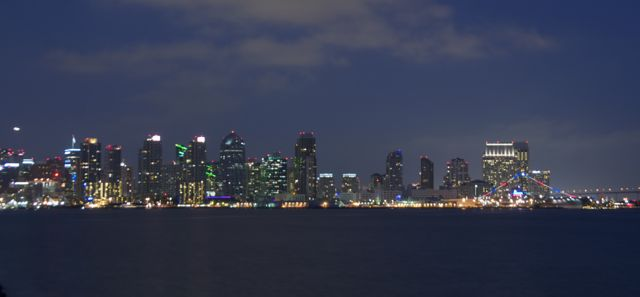
\includegraphics[width=0.5\textwidth]{sandiego}
  \caption[A picture of San Diego. Short figure caption must be \protect{$< 4$} lines in the list of figures]
{A picture of San Diego.  Short figure caption must be \protect{$< 4$} lines in the list of figures and match the start of the main figure caption verbatim. Note that figures must be on their own line (no neighboring text) and captions must be single-spaced and appear \protect\textit{below} the figure.  Captions can be as long as you want, but if they are longer than 4 lines in the list of figures, you must provide a short figure caption.\index{SanDiego}}
  \label{fig:sandiego}
\end{figure}
\chapter{Clio}

This is only a test.
\section{A section}
Test.

\subsection{A Figure Example}
\label{ssec:figure_example}

This subsection shows a sample figure.

\begin{figure}[h] 
  \centering
  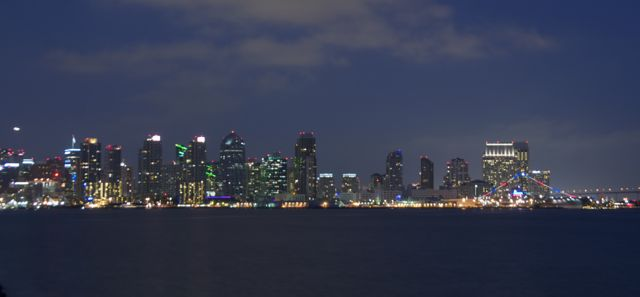
\includegraphics[width=0.5\textwidth]{sandiego}
  \caption[A picture of San Diego. Short figure caption must be \protect{$< 4$} lines in the list of figures]
{A picture of San Diego.  Short figure caption must be \protect{$< 4$} lines in the list of figures and match the start of the main figure caption verbatim. Note that figures must be on their own line (no neighboring text) and captions must be single-spaced and appear \protect\textit{below} the figure.  Captions can be as long as you want, but if they are longer than 4 lines in the list of figures, you must provide a short figure caption.\index{SanDiego}}
  \label{fig:sandiego}
\end{figure}
\chapter{Disaggregating and Consolidating Network Functionalities with SuperNIC}

\section{Introduction}
\label{sec:snic:intro}

{\em Hardware resource disaggregation} is a solution that decomposes full-blown, general-purpose servers into segregated, network-attached hardware resource pools, each of which can be built, managed, and scaled independently. With disaggregation, different resources can be allocated from any device in their corresponding pools, exposing vast amounts of resources to applications and at the same time improving resource utilization. Disaggregation also allows data-center providers to independently deploy, manage, and scale different types of resources.
Because of these benefits, disaggregation has gained significant traction from both academia~\cite{Shan18-OSDI,FireBox-FASTKeynote,Tsai20-ATC,Nitu18-EUROSYS,DDC-hotcloud20,AIFM,Semeru,kona,InfiniSwap,FastSwap} and industry~\cite{HP-TheMachine,IntelRackScale,alibaba-polardb,facebook-disaggregation,SnowFlake-NSDI20}.

While increasing amounts of effort go into disaggregating compute~\cite{Shan18-OSDI,disagg-gpu}, memory (or persistent memory)~\cite{Shan18-OSDI,HP-TheMachine,Lim09-disaggregate,remote-region-atc18,Tsai20-ATC,Semeru,InfiniSwap,FastSwap,hotpot-socc17}, and storage~\cite{PolarFS-VLDB18,SnowFlake-NSDI20,hailstorm-asplos20,ana-eurosys16,gimbal}, the fourth major resource, \textit{network}, has been completely left out.
At first glance, ``network'' cannot be disaggregated from either a traditional monolithic server or a disaggregated device (in this paper collectively called {\em endpoints}), as they both need to be attached to the network.        
%To answer this question, we explore the minimal network functionalities an endpoint needs to have for its connectivity.
%\bolditpara{Proposal: what can be disaggregated?}
However, we observe that even though endpoints need basic connectivity, it is not necessary to run {\em network-related tasks} at the endpoints.
These network tasks, or {\em \nt}s, include the transport layer and all high-level layers such as network virtualization, packet filtering and encryption, and application-specific functions.
%everything including and above the transport layer can 
%each endpoint only needs to manage the connectivity and reliability of the {\em last hop} --- between the endpoint to its direct connection point, and thus only needs a link layer that can handle problems happening within the last hop.
%\noteys{the above reasoning does not make sense to me. we don't have enough context to setup "last hop".}
%Everything else can be disaggregated, including a transport layer for reliable end-to-end delivery, network functions like packet filtering and network virtualization, and application-specific functionalities such as data caching. We collectively call all these ``detachable'' functionalities {\em network tasks}, or {\em \nt}s.

This paper, for the first time, proposes the concept of {\em network disaggregation} and builds a real disaggregated network system to segregate \nt{}s from endpoints.
%systematically answers a set of key questions in network disaggregation.

%\bolditpara{Proposal: disaggregated network resource pool.}
At the core of our network-disaggregation proposal is the concept of a rack-scale disaggregated {\em network resource pool}, which consists of a set of hardware devices that can execute \nt{}s and collectively provide ``network'' as a service (Figure~\ref{fig-snic-topology}), similar to how today's disaggregated storage pool provides data storage service to compute nodes. 
Endpoints can offload (\ie, disaggregate) part or all of their \nt{}s to the network resource pool.
After \nt{}s are disaggregated, we further propose to {\em consolidate} them by aggregating a rack's endpoint \nt{}s onto a small set of network devices.
%\notearvind{might need to generalize to a network pool}
%, thereby reducing the total number of network .

We foresee two architectures of the network resource pool within a rack. The first architecture inserts a network pool between endpoints and the ToR switch by attaching a small set of endpoints to one network device, which is then connected to the ToR switch (Figure~\ref{fig-snic-topology} (a)). The second architecture attaches the pool of network devices to the ToR switch, which then connects to all the endpoints (Figure~\ref{fig-snic-topology} (b)). 

%\bolditpara{Motivating: what are the potential benefits of disaggregating and consolidating \nt{}s?}
%Same as disaggregating other resources like storage, 
Network disaggregation and consolidation have several key benefits.
(1) Disaggregating \nt{}s into a separate pool allows data center providers to build and manage network functionalities only at one place instead of at each endpoint. 
This is especially helpful for heterogeneous disaggregated clusters where a full network stack would otherwise need to be developed and customized for each type of endpoint.
(2) Disaggregating \nt{}s into a separate pool allows the {\em independent scaling} of hardware resources used for network functionalities without the need to change endpoints.
(3) Each endpoint can use more network resources than what can traditionally fit in a single NIC. 
(4) With \nt\ consolidation, the total number of network devices can be reduced, allowing a rack to host more endpoints.
%The final and important benefit comes from consolidation.
(5) The network pool only needs to provision hardware resources for the peak \textit{aggregated} bandwidth in a rack instead of each endpoint provisioning for its own peak, reducing the overall CapEx cost.

Before these benefits can be exploited in a real data center, network disaggregation needs to first meet several goals, which no existing solutions fully support (see \S\ref{sec:snic:related}).

{
\begin{figure}
\begin{center}
\centerline{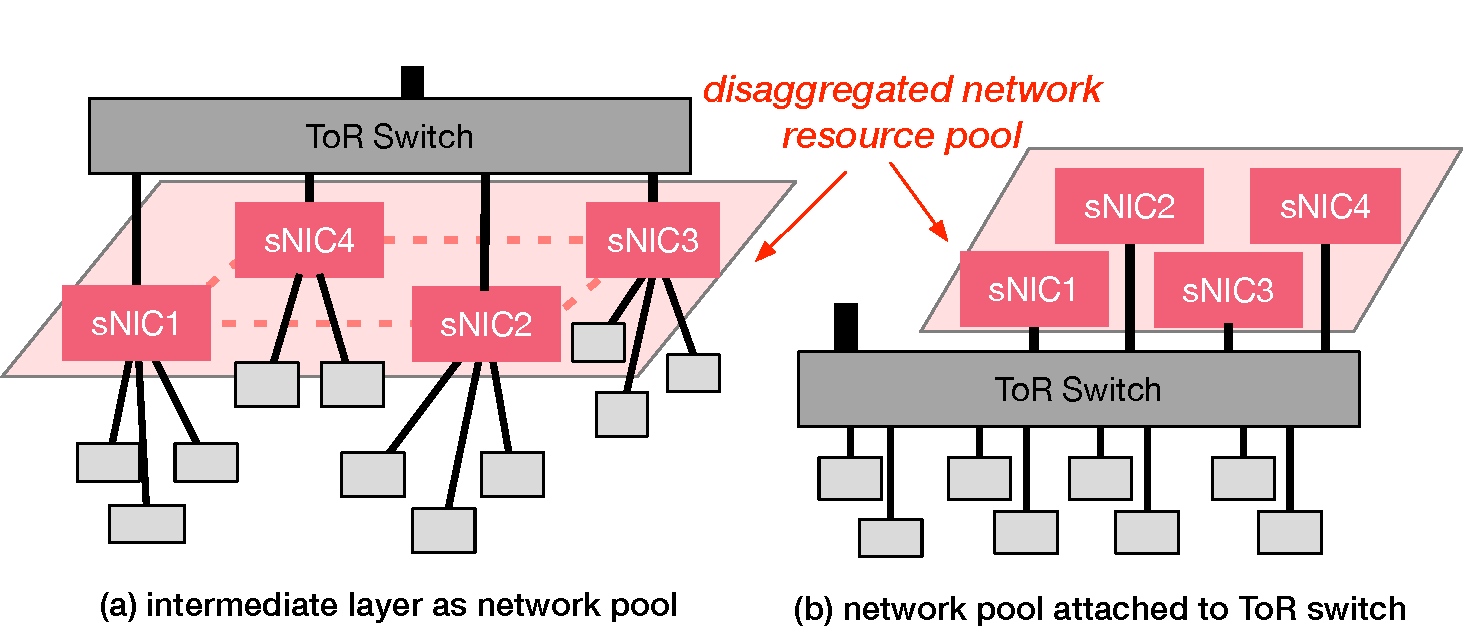
\includegraphics[width=\columnwidth]{Figures/fig-topology.pdf}}
\vspace{-0.1in}
\mycaption{fig-topology}{Overall Architectures of \sysname.}
{
Two ways of connecting \snic{}s to form a disaggregated network resource pool. In (a), dashed lines represent links that are optional.
%\yizhou{can we use another color set for this fig?}
}
\end{center}
\vspace{-0.2in}
\end{figure}
}


%\bolditpara{Building: what are the key requirements of network disaggregation and consolidation?}
First, each disaggregated network device should meet endpoints' original performance goals even when handling a much larger (aggregated) load than what each endpoint traditionally handles.
The aggregated load will also likely require many different \nt{}s, ranging from transports to application-specific functionalities.
Moreover, after aggregating traffic, there are likely more load spikes (each coming from a different endpoint) that the device needs to handle.

Second, using a disaggregated network pool should reduce the total cost of a cluster. This means that each disaggregated network device should provision the right amount of hardware resources (CapEx) and use as little of them as needed at run time (OpEx). At the same time, the remaining part of a rack (\eg, endpoints, ToR switch, cables) needs to be carefully designed to be low cost.

Third, as we are consolidating \nt{}s from multiple endpoints, in a multi-tenant environment, there would be more entities that need to be isolated. We should ensure that they fairly and safely share various hardware resources in a disaggregated network pool. 

Finally, network devices in a pool need to work together so that lightly loaded devices can handle traffic for other devices that are overloaded.
This load balancing would allow each device to provision less hardware resources as long as the entire pool can handle the peak aggregated load of the rack.

%key challenges consolidation
%sharing, autoscaling, dist
%control plane scalability

Meeting these requirements together is not easy as they imply that the disaggregated network devices need to use minimal and properly isolated hardware resources to handle large loads with high variation, while achieving application performance as if there is no disaggregation.

To tackle these challenges and to demonstrate the feasibility of network disaggregation, we built \textit{\textbf{SuperNIC}} (or \textit{\snic} for short), a new hardware-based programmable network device designed for network disaggregation.
%why new hardware-based sNIC. functions like transport need high speed parallel processing, and software is too slow for that. however, traditional NIC hardware or hardware-based SmartNIC does not offer the autoscaling or fair sharing feature we need for consolidation.
An \snic\ device consists of an ASIC for fixed systems logic, FPGA for running and reconfiguring \nt{}s, and software cores for executing the control plane.
We further built a distributed \snic\ platform that serves as a disaggregated network pool.
Users can deploy a single \nt\ written for FPGA or a directed acyclic graph (DAG) execution plan of \nt{}s to the pool.

To tightly \textbf{consolidate} \nt{}s within an \snic, we support three types of resource sharing: (1) splitting an \snic's hardware resources across different \nt{}s ({\em space sharing}), (2) allowing multiple applications to use the same \nt{} at different times ({\em time sharing}), and (3) configuring the same hardware resources to run different \nt{}s at different times ({\em time sharing with context switching}).
For space sharing, we partition the FPGA space into {\em region}s, with each hosting one or more \nt{}s.
Each region could be individually {\em reconfigured} (via FPGA partial reconfiguration, or {\em PR}) for starting new \nt{}s or to context switch \nt{}s.
Different from traditional software systems, hardware context switching with PR is orders of magnitude slower, which could potentially impact application performance significantly.
To solve this unique challenge, we propose a set of policies and mechanisms to reduce the need to perform PR or to move it off the performance-critical path, \eg, by keeping de-scheduled \nt{}s around like a traditional victim cache, by not over-reacting to load spikes, and by utilizing other \snic{}s when one \snic\ is overloaded.
%\notearvind{Might be worth saying that we also rely on other sNICs' resources if a local sNIC is overloaded.}

To achieve high \textbf{performance} under large, varying load with minimal cost, we automatically scale (auto-scale) an \nt{} by adding/removing instances of it and sending different flows in an application across these instances.
%\noteyiying{@Yizhou, do we send different flows to different instances or it's packet level? --- YS: We use flows. We cannot do individual packet LB, because there are states associated with each flow.}
We further launch different \nt{}s belonging to the same application in parallel and send forked packets to them in parallel for faster processing.
%We achieve high throughput using two levels of parallelism:
%{\em \nt{} parallelism} where a packet goes through multiple \nt{}s in parallel and {\em instance parallelism} where we launch multiple instances of the same \nt{} to handle different packets in an application.
%Apart from the above data-plane designs, we build a scalable control plane.
%To achieve low scheduling latency and scalability, we 
%propose a scheduler that centers around a new notion, {\em \nt\ chaining}.
%The idea is to 
To achieve low scheduling latency and improve scalability, we group \nt{}s that are likely to be executed in a sequence into a chain.
% and to have our central scheduler schedule packets only once for the entire chain. 
Our scheduler reserves credits for the entire chain as much as possible so that packets execute the chain as a whole without involving the scheduler in between.
%Doing so improves both packet-processing latency and scheduler scalability.

To provide \textbf{fairness}, we adopt a fine-grained approach that treats each internal hardware resource separately, \eg, ingress/egress bandwidth, internal bandwidth of each shared \nt, payload buffer space, and on-board memory, as doing so allows a higher degree of consolidation.
%Our context is unique in that the packet processing system itself requires multi-dimensional resource sharing. 
We adopt Dominant Resource Fairness (DRF)~\cite{DRF} for this multi-dimensional resource sharing.
%For the first time in networking systems, we consider multi-dimensional resource sharing and provide Dominant Resource Fairness (DRF)~\cite{DRF}. 
Instead of user-supplied, static per-resource demands as in traditional DRF systems, we monitor the actual load demands at run time and use them as the target in the DRF algorithm.
Furthermore, we propose to use ingress bandwidth throttling to control the allocation of other types of resources.
We also build a simple virtual memory system to \textbf{isolate and protect} accesses to on-board memory. %All \nt's memory accesses use 

Finally, for \textbf{distributed \snic{}s}, we automatically scale out \nt{}s beyond a single \snic\ when load increases and support different mechanisms for balancing loads across \snic{}s depending on the network pool architectures.
For example, with the switch-attached pool architecture, we use the ToR switch to balance all traffic across \snic{}s.
With the intermediate pool architecture, we further support a peer-to-peer, \snic-initiated load migration when one \snic\ is overloaded.

We prototype \snic\ with FPGA using two 100\Gbps, multi-port HiTech Global HTG-9200 boards~\cite{htg9200}.
%The data plane runs on FPGA directly, while the control plane runs in software cores deployed on FPGA.
We build three types of \nt{}s to run on \snic:
reliable transport, traditional network functions, and application-specific tasks, and port two end-to-end use cases to \snic.
The first use case is a key-value store we built on top of real disaggregated memory devices~\cite{Clio}.
We explore using \snic{}s for traditional \nt{}s like the transport layer and customized \nt{}s like key-value data replication and caching.
%For the latter, the client only needs to send one copy to the \snic, which will send copies of the data to multiple memory devices.
%customized network abstraction for disaggregated memory device: a key-value store interface (rather than the standard messaging interface).
%Furthermore, we 
The second use case is a Virtual Private Cloud application we built on top of regular servers by connecting \snic{}s at both the sender and the receiver side.
We disaggregate \nt{}s like encapsulation, firewall, and encryption to the \snic{}s.
%a go-back-N reliable transport; a set of network functions including firewall, AES encryption, and VPN Gateway; and a set of application-specific functions including key-value store replication and caching.
We evaluate \snic\ and the ported applications with micro- and macro-benchmarks and compare \snic\ with no network disaggregation and disaggregation using alternative solutions such as multi-host NICs and a recent multi-tenant SmartNIC~\cite{panic-osdi20}.
Overall, \snic\ achieves 52\% to 56\% CapEx and OpEx cost savings with only 4\% performance overhead compared to a traditional non-disaggregated per-endpoint SmartNIC scenario.
%Our results running a Facebook key-value trace~\cite{Atikoglu12-SIGMETRICS} show that \snic's consolidation of four endhosts and two \nt{}s saves 64\% costs compared to no consolidation, with only 1.3\% performance overhead.
Furthermore, the customized key-value store caching and replication functionalities on \snic\ improves throughput by 1.31\x\ to 3.88\x\ and latency by 1.21\x\ to 1.37\x\ when compared to today's remote memory systems with no \snic.
\section{Motivation and Related Works}
\label{sec:motivation}

\subsection{Benefits of Network Disaggregation}
\label{sec:benefits}
As discussed in \S\ref{sec:intro}, disaggregating network functionalities into a separate pool has several key benefits for data centers, some of which are especially acute for future disaggregated, heterogeneous data centers~\cite{LegoOS,last-cpu-hotos, FratOS-eurosys}.

\bolditpara{Flexible management and low development cost.}
Modern data centers are deploying an increasing variety of network tasks to endpoints, usually in different forms (\eg, software running on a CPU, fixed-function tasks built as ASIC in a NIC, software and programmable hardware deployed in a SmartNIC). 
It requires significant efforts to build and deploy them to different network devices on regular servers and to different types of disaggregated hardware devices.
After deployment, configuring, monitoring, and managing them on all the endpoints is also hard.
%, even in a homogeneous cluster.
In contrast, developing, deploying, and managing network tasks in a disaggregated network pool with homogeneous devices is easy and flexible.

\bolditpara{Independent scaling.}
It is easy to increase/decrease network hardware resources in a disaggregated network pool by adding/removing network devices in the pool. Without disaggregation, changing network resources would involve changing endpoints (\eg, upgrading or adding NICs).

\bolditpara{Access to large network resources.}
With disaggregation, an endpoint can potentially use the entire network pool's resources, far beyond what a single NIC or server can offer.
This is especially useful when there are occasional huge traffic spikes or peak usages of many \nt{}s.
Without network disaggregation, the endpoint would need to install a large NIC/SmartNIC that is bloated with features and resources not commonly used~\cite{SmartNIC-nsdi18,Caulfield-2018}.

Beside the above benefits, a major benefit of network disaggregation is cost savings. A consolidated network pool only needs to collectively provision for the peak aggregated traffic and the maximum total \nt{}s used by the whole rack at any single time.
In contrast, today's non-disaggregated network systems require each endpoint to provision for its individual peak traffic and maximum \nt{}s.
To understand how significant this cost is in the real world, we analyze a set of traces from both traditional server-based production data centers and disaggregated clusters.

\bolditpara{Server-based data center traffic analysis.}
To understand network behavior in server-based data centers, we analyze two sets of traces: a Facebook trace that consists of Web, Cache, and Hadoop workloads~\cite{facebook-sigcomm15}, and an Alibaba trace that hosts latency-critical and batch jobs together~\cite{alibaba-trace}. 

We first perform a consolidation analysis where we calculate the sum of peaks in each individual endhost's traffic (sum of peak) and the peak of aggregated traffic within a rack and across the entire data center (peak of sum). 
These calculations model the cases of no disaggregation, disaggregation and consolidation at the rack level and at the data-center level.
%The former informs us about the total amount of network resources that needs to be provisioned if each endhost provisioned for its own peak, and the latter corresponds to the amount of resources a disaggregated network pool needs to provision.
Figure~\ref{fig-fb-alibaba} shows this result for the two data centers. 
For both of them, a rack-level consolidation consumes one magnitude fewer resources than no consolidation.

We then analyze the load spikes in these traces
%Our first finding is that \fixme{XXX}\% and \fixme{XXX}\% spikes are at least one and two seconds long.
by comparing different endhosts' spikes and analyzing whether they spike at similar or different times, which will imply how much chance there is for efficient consolidation.
Specifically, we count how much time in the entire 1-day trace $X$ number of endhosts spike together.
Figure~\ref{fig-spike-var} shows that 55\% of the time only one or two servers spike together, and only 14\% of the time four or more servers spike together.
This result shows that servers mostly spike at different times, confirming the large potential of consolidation benefits.
%\ryan{We analyze the portion of time N servers are spiking for a given time period. Figure~\ref{fig-spike-var} shows that 55\% of the time 1 to 2 servers are peaking. And only 14\% of the time do 4 servers peak concurrently.
%Overall, it confirms that although individual server's traffic is spiky, the correlation among servers is low and the number of servers concurrently peaking is small.}
%
%Both data centers exhibit high burstiness, and bursts happen at different times for different end hosts. % 
%Other prior work has also reported similar findings~\cite{netkernel-atc20,Gao16-OSDI}.

\bolditpara{Disaggregated cluster traffic analysis.}
Resource disaggregation introduces new types of network traffic that used to be within a server, \eg, a CPU device accesses data in a remote memory device. 
If not handled properly, such traffic could add a huge burden to the data-center network~\cite{sirius-sigcomm20}.
To understand this type of traffic, we analyzed a set of disaggregated-memory network traces collected by Gao et al. using five endhosts~\cite{Gao16-OSDI}.
Figure~\ref{fig-OSDI16NetTrace} plots the CDF and the timeline of network traffic from four workloads.
These workloads all exhibit fluctuating loads, with some having clear patterns of high and low load periods.
We further perform a similar analysis using sum of peaks vs. peak of aggregated traffic as our server-based trace analysis.
Consolidating just five endhosts already results in 1.1\x\ to 2.4\x\ savings with these traces.





\subsection{Limitations of Alternative Solutions}
\label{sec:related}

The above analysis makes a case for disaggregating and consolidating network tasks from individual servers and devices.
A question that follows is \textit{where} to host these \nt{}s and whether existing solutions could achieve the goals of network disaggregation and consolidation.
%\notearvind{I will refine this a bit more and see whether Gimbal should be incorporated here or somewhere else.}

%\noteys{different from the p4 switch, the aruba switch seems another type of programmable switch that maybe able to support more complex ops}
%
The first possibility is to host them at a \textbf{programmable ToR switch}. Programmable switches allow for configurable data planes, but they typically support only a small amount of computation at high line rates. SmartNICs, on the other hand, handle more stateful and complex computations but at lower rates. Transport protocol processing and encrypted communications are examples of complex network tasks better supported by a SmartNIC than a programmable switch. Moreover, existing programmable switches lack proper multi-tenancy and consolidation support~\cite{Wang-HotCloud20}. As a consequence, most data center designs require the use of SmartNICs even in the presence of programmable switches, and our proposal simply disaggregates SmartNIC-like capabilities into a consolidated tier.


Another possibility is upcoming \emph{multi-host SmartNICs} (e.g., Mellanox BlueField3) that are enhancements of today's \textbf{multi-host NICs}~\cite{ocp-nic,Intel-RedRockCanyon}. These NICs connect to multiple servers via PCIe connections and provide general-purpose programmable cores. Our work identifies three key extensions to such devices. (1) Our approach enables a greater degree of aggregation as we enable coordinated management of a distributed pool of network devices. (2) Moreover, in the case of these multi-host SmartNICs, \nt{}s that cannot be mapped to the NIC's fixed functions have to be offloaded as software. In contrast, \snic\ allows the acceleration of \nt{}s in hardware, enabling higher performance while tackling issues related to runtime reconfigurability of hardware. (3) Our approach provides adaptive mechanisms for adjusting to workloads and providing fair allocation of resources across applications. It is also worth noting that (1) and (3) can by themselves be used in conjunction with commercial multi-host SmartNICs to achieve a different software-based instantiation of our vision.
%\noteys{"multi-host SmartNICs support NT offloading only in software", not quite true. those smartNICs have ASIC NFs and FPGA (like IPU). its better to mention MH-NIC are generally used to offload software NTs.}\notearvind{Reworded it a bit. Specified the possibility of fixed functions. Also narrowly defined it as SmartNICs with programmable cores. BTW, I don't think I have seen a MH-Innova, which would be the closest to our system.}

\textbf{Middleboxes} are a traditional way of running network functions inside the network either through hardware black-box devices that cannot be changed after deployment~\cite{aplomb-sigcomm20,comb-nsdi12,walfish-osdi04} or through server-based Network Function Virtualization (NFV) that enables flexible software-based middleboxes~\cite{clickos-nsdi14,e2-sosp15,metron-nsdi18,NFP-sigcomm17,parabox-sosr17}, but at the cost of lower performance~\cite{netbricks,netvm-nsdi14}.  Our deployment setting differs from traditional datacenter middleboxes: we target "nearby" disaggregation, as in the endhost or SmartNIC tasks are disaggregated to a nearby entity typically located on the same rack. Consequently, our mechanisms are co-designed to take advantage of this locality (e.g., we use simple hardware mechanisms for flow control between the end-host and the disaggregated networking unit). Further, we target network functionality that is expected either at the endhost itself or at the edge of the network, such as endhost transport protocols, applying network virtualization, enhancing security, which all require nearby disaggregation and are also not typically targeted by middleboxes. We do note that our dynamic resource allocation mechanisms are inspired by related NFV techniques, but we apply them in the context of reconfigurable hardware devices.


%\yiying{Also mention our distributed pooling idea which is not in any of the above existing solutions (maybe need to mention works that use distributed programmable switches/SmartNICs if any)}


%Apart from our \snic\ proposal, there are several options.

% The first possibility is to host them at the \textbf{ToR switch}.
% This approach lets endpoints go through only one hop to the ToR switch, compared to two hops with approaches that use a middle layer like \snic.
% However, it requires ToR switches to be programmable and have more ports to connect to disaggregated devices, both of which add monetary costs and requires changes to the data-center network infrastructure~\cite{zhao-nsdi19,zhang-nsdi19}.
% Moreover, existing programmable switches lack proper multi-tenancy and consolidation support~\cite{Wang-HotCloud20}.  %such as flexible space and time sharing
%\yizhou{maybe build the relation to in-network computing (INC)? traditional pswitch work like netchain/netkv/ATP offload certain app functionlaties to the network. it is a specific case of network-disaggregation-and-consolidation. And we are proposing a larger-scope and more generic scheme.}



% \textbf{Middleboxes} are a traditional way of running network functions inside the network.
% Traditional hardware middleboxes are specialized black-box devices that cannot be changed after deployment~\cite{aplomb-sigcomm20,comb-nsdi12,walfish-osdi04}. Network Function Virtualization uses regular servers to build flexible software-based middleboxes~\cite{clickos-nsdi14,e2-sosp15,metron-nsdi18,NFP-sigcomm17,parabox-sosr17}, but at the cost of running at lower performance~\cite{netbricks,netvm-nsdi14}. 
% \snic\ has the benefits of both: it is flexible as it supports offloading a wide range of \nt{}s and can be reconfigured at run time, and it also achieves high-bandwidth line rate processing.

%Increasing amount of data centers attach \textbf{SmartNICs} and \textbf{specialized ASIC/FPGA devices} like Intel IPU~\cite{intel-ipu}, Amazon Nitro~\cite{aws-nitro}, and Microsoft Catapult~\cite{Catapult-v2} to single servers.
%These devices can host offloaded network functions and other customized tasks. However, they do not support the consolidation of multiple endpoints.

\if 0
Optical circuit switch is an emerging solution to build disaggregated datacenters as it offers high port count and consumes much less energy than traditional electrical packet switches~\cite{shoal-nsdi19,helios-sigcomm10,sirius-sigcomm20, sipml-sigcomm21}. Circuit switch reconfigures and reconnects physical connections among ports. As a result, it has no computation on its data path, thus not able to consolidate any network functions.
\fi

Finally, there are emerging \textbf{interconnections designed for disaggregated devices} such as Gen-Z~\cite{GenZ} and CXL~\cite{CXL}.
These solutions mainly target the coherence problem where the same data is cached at different disaggregated devices.
The transparent coherence these systems provide requires new hardware units at every device, in addition to a centralized manager.
\snic\ supports the disaggregation and consolidation of all types of network tasks and does not require specialized units at endpoints.

%In summary, although different existing network solutions provide some features of network disaggregation and consolidation, none of them meet all our target goals, thus necessitating the design of a new network solution.
%{
\begin{table*}[th]\smallsize
\begin{center}
\begin{tabular}{ p{1.7in} | p{0.5in} | p{0.85in} | p{0.6in} | p{0.55in} | p{0.8in}  | p{0.7in} }

\textbf{Solution} & \textbf{Port Count \textasteriskcentered} & \textbf{Heterogeneous End-Points \textasteriskcentered} & \textbf{Offloaded Transport} & \textbf{Network Function} & \textbf{Manageability} & \textbf{Consolidated Resources} \\
\hline
\hline
Programmable Switch~\cite{RMT-SIGCOMM13,netcache-sosp17} & \xmark & \cmark & \cmark & \cmark  & $\bigcirc$  & $\bigcirc$ \\
\hline
Circuit Switch~\cite{sirius-sigcomm20,shoal-nsdi19,dRedBox-DATE} & \cmark & \cmark & \xmark & \xmark  & \xmark  &\xmark \\
\hline
Coherent Fabrics~\cite{GenZ,CXL,CCIX} & $\bigcirc$ & \cmark & \xmark & \xmark & \xmark & \xmark\\
\hline
Middleboxes~\cite{walfish-osdi04,comb-nsdi12,aplomb-sigcomm20} & \xmark  & \xmark  & \xmark & \cmark & \xmark  & \cmark  \\
\hline
NFV~\cite{clickos-nsdi14,e2,netbricks} & \xmark  & \xmark  & \xmark & \cmark & \cmark & \cmark \\
\hline
Multi-Host NIC~\cite{Intel-RedRockCanyon,Mellanox-Multihost} & \cmark &  $\bigcirc$ & \xmark & \xmark & \xmark  & $\bigcirc$ \\
\hline
\hline
\textbf{\sysname}     & \cmark & \cmark &  \cmark & \cmark & \cmark & \cmark \\
\hline
\end{tabular}
\end{center}
\mycaption{tabel-related-work}{Comparison of Network Solutions.}
{
\textasteriskcentered\ features only applicable to disaggregated datacenters.
$\bigcirc$ partially support.
}
\end{table*}
}








\if 0
\subsection{for Server-Based Datacenters}
\label{sec:motivation-server}
%scale, computation tax, underutilization etc.

%Today, each server runs a full network stack (either in the host CPU or in a NIC), and many start to execute complex network functions and application-specific tasks~\cite{flexnic-asplos16,snap-sosp19}.
%(\eg, FlexNIC~\cite{flexnic} demonstrates the benefits of application-specific network handling and iPipe~\cite{iPipe} factors out a distributed application into a collection of actor-based NFs). 
%Network stacks in today's data centers could consume 30\%-40\% host CPU cycles with the presence of a high-speed network~\cite{tonic-nsdi20}.
%However, network communication only happens for a small amount of time during application execution, and not all network functions are always invoked. 
%
To understand network behavior in real, server-based data centers, we analyze two sets of traces: a Facebook trace that consists of Web, Cache, and Hadoop workloads~\cite{facebook-sigcomm15}, and an Alibaba trace that hosts latency-critical and batch jobs together~\cite{alibaba-trace}. 
Both data centers exhibit high burstiness, and bursts happen at different times for different end hosts. Other prior work has also reported similar findings~\cite{netkernel-atc20,Gao16-OSDI}. We omit the CDF and timeline plots due to space constraints. 
We perform a similar consolidation analysis as the disaggregated memory traces, as shown in Figure~\ref{fig-fb-alibaba}. 
%Specifically, we first measure the peak load of every end host and then sum all these peaks across the whole data center (or in Facebook's case, an entire workload). This case uses no consolidation (\ie, today's scheme) and the sum is the total amount of resources that a data center needs to provision.
In addition to the sum of individual-endhost peaks and the peak of aggregated traffic across the entire data center (or, in Facebook's case, an entire workload),
%we model the case where each rack's network traffic could be handled in a consolidated way (\eg, with \snic{}s). We first
we sum the traffic under a rack %for each time point and then measure the peak of the summed traffic. Afterwards, we 
and sum all the per-rack peaks.
%Finally, we model the unrealistic case of consolidating the entire data-center's traffic by summing the traffic of the whole data center at each time point and then measuring the peak of the sums.
For both Facebook and Alibaba, rack-level consolidation consumes one to two orders of magnitude fewer resources than no consolidation.


\if 0
We measure the duration of high-intensity communications or bursts at 25\mus\ granularity.
%We say that a switch's egress link is \textit{hot} if, for the measurement period, its utilization exceeds 50\%. An unbroken sequence of hot samples indicates a \textit{burst}. 
Figure~\ref{fig-burst_duration} presents the CDF of burst durations across three workloads.  We observe that a significant fraction of these bursts are only one sampling period long. The 90th percentile duration is less than 200\mus\ for all three rack types.
%, with Web racks having the lowest 90th percentile burst duration at 50us (two sampling periods). Hadoop racks have the longest tail of the three, but even then, almost all bursts concluded within 0.5\,ms.
The results indicate that bursts not only exist, almost all high utilization at the edge of the data center network is part of a burst, and that the durations of these high-intensity communications is short.
\fi

In addition to the bursty traffic patterns that are conducive to the consolidation benefits of \sysname,
the under-utilization of network functions in today's network devices is another major motivation for \sysname. 
For example, existing NICs are bloated with features that are not utilized in the common case~\cite{SmartNIC-nsdi18,Caulfield-2018}. 
Wang et al.~\cite{Wang-HotCloud20} reported that state-of-the-art programmable switches have low resource utilization (common NFs consume less than 1\%), 
and even a complex application consumes only a small fraction of resources (\eg, NetChain~\cite{netchain-nsdi18} uses 3\% MAT resources). 
Over time, vendors keep adding more features into their network device products to meet the diverse requirements from different customers, resulting in significant resource waste that could otherwise be avoided by \sysname's consolidation solution. 

% Crucially, for both cases above, the consolidation enables statistical multiplexing of resources that allows us to move away from provisioning for peak utilization on a per-node basis to provisioning for the expected peak utilization on a rack basis.
Finally, consolidating network tasks into a separate pool makes it easy for datacenter operators to manage them (\eg, monitoring, reconfiguring, and upgrading).

%The offloading of the network stack and host-side network functions (\eg, Open vSwitch) to the \snic{} has associated cost savings as we can substitute the use of expensive x86 cores with cheaper circuitry at the \snic.  Moreover, in all of these cases, network consolidation allows us to provision less networking associated compute resources at the \snic{} when compared to the traditional non-consolidated deployment. 


\subsection{for Disaggregated Datacenters}

Resource disaggregation is a data-center architecture that organizes different hardware resources into separate, network-attached pools.
While today's data centers use regular servers to form these pools~\cite{alibaba-polardb,SnowFlake-NSDI20,Borg-eurosys20}, 
future data centers could benefit from using specialized {\em devices} to build such pools, \eg, a memory pool consisting of network-attached memory~\cite{clio-arxiv} or Optane boards~\cite{HP-TheMachine,ATC20-pDPM}.
Three practical and key technical hurdles need to be solved before data centers can readily deploy such device-based disaggregated resource pools. Network disaggregation solves all of them.


%More data centers are migrating to a disaggregated architecture where different resources are managed as individual, network-attached pools~\cite{Alibaba,Facebook,snowflake-nsdi20,google-paper,XXX}.
%Nodes in a resource pool can both be a regular server (\eg, a server dedicated to provide data storage~\cite{snowflake-nsdi20,XXX}) or a network-attached device (\eg, a persistent-memory device board~\cite{HP-TheMachine,XXX}).
%There is a growing demand for deploying specialized devices (such as memory devices, network-attached NVMes, and key-value storage devices) inside the data center. 

%Network disaggregation is especially useful in building and deploying such disaggregated devices by solving three key problems at the same time.
First, when a monolithic server is replaced with multiple network-attached disaggregated devices (\eg, one CPU processor, one memory device, one storage device to replace a server), the number of network endpoints could increase to hundreds per rack~\cite{shoal-nsdi19}. % and an order of magnitude more than what a ToR switch could handle).
If all these devices directly connect to a ToR switch, the rack needs to use an expensive, high-port-count ToR switch or multiple low-port-count ToR switches (and the resulting increased scale of the entire switch hierarchy~\cite{zhang-nsdi19,zhao-nsdi19}).
%, and all the network infrastructure above ToR switches may also need to be upgraded.
With our proposed architecture, devices in a rack connect to a small set of \snic{}s that then can be accommodated by today's data-center ToR switch.
%, thus requiring no network infrastructure changes in existing data centers.

Second, building different types of disaggregated devices involves adding standard networking functionalities like a reliable transport layer to each of them, with many of them also desiring various customized network functions.
Disaggregated devices will come in many forms, some with a software processor~\cite{LegoOS}, some with only hardware units~\cite{ATC20-pDPM}, and some with both software and hardware~\cite{clio-arxiv}. Designing and implementing network tasks in each type of disaggregated device will be a daunting job. Moreover, it likely will involve adding additional hardware units to the devices.
By building \nt{}s once for a single type of hardware (\ie, \snic), we could significantly save development and CapEx costs.
%that would otherwise be required at every disaggregated device.
%three types of costs in a disaggregated device:
%{\em development cost} to build network stacks in heterogeneous hardware (\eg, ASIC, FPGA, general-purpose processor),
%{\em CapEx cost} for additional hardware network units in each device,
%and {\em energy cost} to run the network stacks there.
%
%Finally, when each device hosts its own network functionalities (and in heterogeneous hardware), 
%managing them will be difficult for data center providers.
%For example, to change the configuration of a network policy or to add a new network
%function to a set of disaggregated devices, each of them needs to change their network
%stack, which is hard and sometimes impossible as devices are often 
%manufactured by different vendors and have their (locked-in) hardware 
%implementations. 
%Network disaggregation makes it easy for operators to manage network functionalities for heterogeneous devices.

Finally, resource disaggregation introduces new types of network traffic that used to be within a server, \eg, a CPU device accesses a remote memory device to read/write data. 
If not handled properly, such traffic could add a huge burden to the data-center network~\cite{sirius-sigcomm20}.
To understand this type of traffic, we analyzed a set of disaggregated-memory network traces collected by Gao et al. using five endhosts~\cite{Gao16-OSDI}.
Figure~\ref{fig-OSDI16NetTrace} plots the CDF and the timeline of network traffic from four workloads.
These workloads all exhibit fluctuating loads, with some having clear patterns of high and low load periods.
We further compare the case where we provision network resources for the peak load of every workload and the case where we could consolidate and only provision for the aggregated network demand (\ie, sum of peaks vs. peak of aggregated traffic).
Consolidating just five endhosts already results in 1.1\x\ to 2.4\x\ savings with these traces.
%Overall, network consolidation allows us to provision for the {\em aggregated peak}, saving both CapEx and OpEx costs.
%The traffic is collected every five seconds.

\fi


\if 0
\section{Network Disaggregation and Consolidation}

%\NOTE{
%This section is similar to the sec2.2 in the proposal.
%1) Define the idea of "Network Disaggregation and Consolidation".
%Define a set of Key Goals: perf, cost, programmbility, consolidation and so on.
%2) present related fields.
%}
We propose to disaggregate and consolidate network functionalities.
The core of \sysname\ is a disaggregated network pool that sits in between endpoints and a ToR switch.
This pool consists of a set of \textit{SuperNICs} (\textit{\snic}s), each of which connects to the ToR switch (up link) and a small set of end hosts (down links).
In addition, all the \snic{}s are connected together through a ring or a torus.
We aim to support three broad types of end hosts:
regular servers, \textit{passive} disaggregated devices which only receive and handle network requests (\eg, a storage device that handles file I/O requests), 
and \textit{active} disaggregated devices which could both initiate and receive network requests (\eg, a memory device that handles memory read/write requests and swaps or flushes its memory data to a storage device).

\textbf{Architecture.}

\textbf{Goals.} A general set of goals, which we should show
that related work cannot meet.

\textbf{Related Work}
\TODO{Optional. We could describe
one system here as an example, leave the whole thing
to Related Work Section.}

\TODO{
Network disaggregation and consolidation is a concept.
SuperNIC is just one implementation choice.
So, before we dive into SuperNIC, we must explain
why SuperNIC, why other solutions cannot work.
Specifically, why not use pSwitch to realize this idea?
Why not use multihost NIC to do this?
We don't need a lengthy exploration here.
}

\fi

\if 0
\subsection{Resource Disaggregation}

A monolithic server has been the unit of deployment and operation
in datacenters for decades. This long-standing server-centric architecture
has several key limitations:
\textit{a) Inefficient resource utilization}. With a server being the physical
boundary of resource allocation, it is difficult to fully utilize all resources
in a datacenter. Reports show Google and Alibaba's datacenter usually only
have 40\%-60\% utilization~\cite{legoOS,Borg-eurosys20}. One of the main
reasons is the constraint that CPU and memory for a job have to be allocated
from the same physical machine.
\textit{b) Poor hardware elasticity}.
It is difficult to add, move, remove, and reconfigure
hardware components after they have been installed in
a monolithic server~\cite{FB-Wedge100}.
However, such plans have to be adjusted frequently because of
today's speed of change in application requirements.
\textit{c) Coarse failure domain}.
The failure unit of monolithic servers is coarse.
When a hardware component within a server fails, the whole
server is often unusable.
\textit{d) Bad support for heterogeneity}.
Driven by application needs, new hardware technologies
are finding their ways into datacenters (e.g., FPGA, GPU, and TPU).
However, datacenters often need to purchase
new servers to host certain hardware.
Other parts of the new servers can go underutilized~\cite{legoOS}.

Resource Disaggregation breaks the monolithic server model,
in which hardware resources in traditional servers are disseminated
into network-attached hardware devices.
Each device has a controller and a network interface,
can operate on its own, is an independent, failure-isolated entity.
The disaggregated approach largely increases the flexibility of a datacenter.
Applications can freely use resources from any hardware device,
which makes resource allocation easy and efficient.
Different types of hardware resources can scale independently.
It is easy to add, remove, or reconfigure devices.
New types of hardware devices can easily be deployed in a datacenter
— by simply enabling the hardware to talk to the network and adding a
new network link to connect it.
Finally, hardware resource disaggregation enables fine-grain failure isolation,
since one device failure will not affect the rest of a cluster

Disaggregation has been a very active research area for the past decade.
It was first proposed in early 2010s for memory disaggregation~\cite{Lim09-disaggregate}.
Over the years, researchers have further explored
disaggregation's impact on
operating system~\cite{legoOS}, storage~\cite{snowflake-nsdi20},
persistent memory~\cite{ATC20-pDPM},
data structure~\cite{aifm-osdi20},
failure model~\cite{disaggregation-hotcloud20}, and many more.
Overall, prior research focuses on the \textit{infrastructure},
as in integrating disaggregation with various existing systems,
thereby lays a solid system-level foundation.
Researchers now gradually shift their focus onto higher level components,
such as programming framework, security, and the focus of this paper, network.
Ultimately, to prepare a complete ecosystem for future disaggregated datacenters.

\subsubsection{Challenges for Network Design}

One of the base designs for disaggregation is that each device has an attached network interface.
However, the fourth major computation resource in datacenter, network, has been completely left out in the process of disaggregation.
The network is facing unprecedented challenges and we think
the disaggregation idea would not be practical if those challenges are not addressed properly

First, when splitting a monolithic server into multiple network-attached
devices, the number of network endpoints will dramatically increase
(potentially hundreds or even thousands of devices per rack~\cite{shoal-nsdi19}).
Attaching those devices directly to Top-of-Rack (ToR) switches are not feasible,
because it would increase the number of ToRs and subsequently spine and core switches dramatically in a Clos-based topology.
This poses a huge impact on existing datacenter networks, in terms of cost, power, and physical upgrade capability,
collectively called the \textit{network scale tax}~\cite{sirius-sigcomm20}.

Second, with the increasing degree of heterogeneity,
it is hard to deploy and run a consistent network stack across all those
heterogeneous disaggregated devices (e.g., ASIC, FPGA, and general-purpose CPUs).
Each device would need a network stack to have reliable connection with others.
Normally the network stack runs on top of a CPU or a programmable NIC,
but this is often not possible for heterogeneous devices.
In addition, driven by application demand, datacenters have the need to update their network
protocols especially congestion control algorithms very frequently~\cite{swift-sigcomm20}.
Thus, the network stack used by disaggregated devices should be universal, consistent
across devices, and easy to upgrade on the field.

Third, the network must provide low latency and high bandwidth for disaggregated devices and their applications.
With emerging applications like distributed ML training running directly on top of disaggregated devices,
network traffic is generated and consumed by hardware directly and hence, is expected
to grow even faster then the current trend (doubling every year~\cite{sirius-sigcomm20}).
Prior work~\cite{legoOS} shows that the network latency should be as low as 5 us to have reasonable performance (i.e., around 20\% slowdown).

\subsection{Current Datacenter Network Limitations}

The network in traditional server clusters are facing numerous
issues and challenges as well. 

As datacenters are moving to 100 Gbps network,
the CPU utilization of software network stacks becomes increasingly prohibitive.
Despite numerous efforts to improve their performance, software network stacks
tend to consume 30-40\% of CPU cycles~\cite{tonic-nsdi20}.

Another major hurdle and motivation for consolidating network resources
is the difficulty of provisioning the right amount of network resources
for individual end hosts (for both regular servers and disaggregated devices).
We will present out preliminary study on this part.
For regular-server clusters, we use traces we have collected from different
workloads (namely Web, Cache, and Hadoop) running inside Facebook datacenters.
We measure the duration of high-intensity communications or bursts at 25 us granularity.
Figure~\ref{fig-burst_duration} presents the CDF of burst duration across three
workloads. We observe that a significant fraction of these bursts are only one
sampling period long.
The 90th percentile duration is less than 200 us for all three rack types.
The results indicate that bursts not only exist, almost all high utilization
at the edge of the datacenter network is part of a burst, and that the duration
of these high-intensity communications is short.
Other prior work has also reported similar findings~\cite{NetKernel-ATC20}.

Disaggregated cluster introduces new types of network traffic,
where devices access other types of devices over the network
(e.g., compute devices accessing remote memory devices).
We use a set of remote memory-swap traces collected by Gao et al.~\cite{Gao16-OSDI}
to model traffic in disaggregated cluster (CDF and time in Figure~\ref{fig-OSDI16NetTrace}).
We observe similar patterns as regular-server clusters, i.e., burst but under-utilized.

In addition to the traffic patterns, under-utilization of network
functionalities in today's network devices is another major issue.
For example, existing NICs are bloated with features are not utilized~\cite{Caulfield-2018,firestone-nsdi18}.
Wang et al.~\cite{wang-hotcloud20} reports that state-of-the-art programmable switches have
low resource utilization, and even a complex application would consume only a small
fraction of resources. In general, vendors keep adding more features into
their network device products to meet the diverse requirements from different
customers, resulting in huge resource waste that could otherwise avoided
by network disaggregation and consolidation.

%{
\begin{table*}[th]\smallsize
\begin{center}
\begin{tabular}{ p{1.7in} | p{0.5in} | p{0.85in} | p{0.6in} | p{0.55in} | p{0.8in}  | p{0.7in} }

\textbf{Solution} & \textbf{Port Count \textasteriskcentered} & \textbf{Heterogeneous End-Points \textasteriskcentered} & \textbf{Offloaded Transport} & \textbf{Network Function} & \textbf{Manageability} & \textbf{Consolidated Resources} \\
\hline
\hline
Programmable Switch~\cite{RMT-SIGCOMM13,netcache-sosp17} & \xmark & \cmark & \cmark & \cmark  & $\bigcirc$  & $\bigcirc$ \\
\hline
Circuit Switch~\cite{sirius-sigcomm20,shoal-nsdi19,dRedBox-DATE} & \cmark & \cmark & \xmark & \xmark  & \xmark  &\xmark \\
\hline
Coherent Fabrics~\cite{GenZ,CXL,CCIX} & $\bigcirc$ & \cmark & \xmark & \xmark & \xmark & \xmark\\
\hline
Middleboxes~\cite{walfish-osdi04,comb-nsdi12,aplomb-sigcomm20} & \xmark  & \xmark  & \xmark & \cmark & \xmark  & \cmark  \\
\hline
NFV~\cite{clickos-nsdi14,e2,netbricks} & \xmark  & \xmark  & \xmark & \cmark & \cmark & \cmark \\
\hline
Multi-Host NIC~\cite{Intel-RedRockCanyon,Mellanox-Multihost} & \cmark &  $\bigcirc$ & \xmark & \xmark & \xmark  & $\bigcirc$ \\
\hline
\hline
\textbf{\sysname}     & \cmark & \cmark &  \cmark & \cmark & \cmark & \cmark \\
\hline
\end{tabular}
\end{center}
\mycaption{tabel-related-work}{Comparison of Network Solutions.}
{
\textasteriskcentered\ features only applicable to disaggregated datacenters.
$\bigcirc$ partially support.
}
\end{table*}
}


\subsection{Disaggregate and Consolidate Network}

To tackle the new network design challenges posed by resource disaggregation
and the limitations of current networks, we propose to disaggregate
and then consolidate the network computation resource into a \textit{network resource pool}.

In this paper, we focus one three types of network functionalities:
1) packet processing logic in NIC hardware,
2) software network stack running at processing units,
3) advanced application-specific network functions.

For disaggregated devices, network disaggregation removes
those network functionalities from the device and replaces a complex NIC
with a simpler one. This step \textit{decouples}
the core device from network and hence, allow them to change and scale independently.

After disaggregation, the network functionalities are further consolidated
into a datacenter-wide network resource pool. This pool provides services
for both disaggregated devices and regular servers.
Essentially, the network resource pool provides \textit{network-as-a-service}.

To the best of our knowledge, no work has attempted
to disaggregate the network before.
At first glance, the network cannot be disaggregated from
either a traditional server or a disaggregated device,
as they both need to be attached to the network and each
endpoint is provisioned with its own network interface and associated
network stacks. So can we disaggregate and then consolidate network?

To answer this question, we need to find out whether
a) it is possible to decouple the network functionalities,
and b) how to build the network resource pool.
In this paper, we focus on the second question.
We review emerging network devices and evaluate whether they
could meet the goals of consolidation and whether they are good
candidates for implementing the network resource pool.

% \subsection{Transports}
% \subsection{Congestion Control}
% \subsection{Network Functions}
% \subsection{Application-Specific Computing}

\fi
\section{SuperNIC Overview}
\label{sec:overview}

%As discussed in \S\ref{sec:related}, although different existing network solutions provide some features of network disaggregation and consolidation, none of them meet all our target goals, thus necessitating the design of a new network solution.
This section gives a high-level overview of the overall architecture of the \snic\ platform and how to use it. %We defer the detailed description of \snic\ design to \S\ref{sec:design} and \S\ref{sec:dist}.

\bolditpara{Overall Architectures.}~~
We support two ways of attaching an \snic\ pool in a rack (Figure~\ref{fig-topology}).
In the first architecture, the \snic\ pool is an intermediate layer between endpoints (servers or devices) and the ToR switch.
Each \snic\ uses one port to connect to the ToR switch.
Optionally, all the \snic{}s can be directly connected to each other, \eg, with a ring topology.
All remaining ports in the \snic\ connect endpoints.
We expect each of these endpoint-connecting links to have high bandwidth (\eg, 100\Gbps) and the uplink to the switch to have the same or slightly higher bandwidth (\eg, 100\Gbps\ or 200\Gbps). 
%Differently, today's multi-host NICs break one link into several sub-links each with a fixed portion of the original link's bandwidth.\notearvind{This is the thing that the reviewer complained about.  Apparently, BF3 has a pcie switch at the ingress that removes this problem. We could skip making this point - but I think that reviewer is not on the SIGCOMM PC!}
%The sum of the link bandwidth at each endpoint that connects to an \snic\ can and should exceed the link bandwidth between the \snic\ and the ToR switch. 
%This is because different endpoints' loads peak at different times (\S\ref{sec:motivation-server}), and after \snic's consolidation, the aggregated traffic would mostly fit the \snic's uplink, as shown in Figure~\ref{fig-fb-alibaba}.
%
The second architecture attaches \snic{}s to the ToR switch, and endpoints directly attach to the ToR switch.
In this architecture, the ToR switch re-directs incoming or outgoing traffic to one or more \snic{}s. 
%and balances load when doing the redirection.
Note that for both architectures, the actual implementation could either package the network pool with the ToR switch to form a new ``switch box'' or be separated out as an pluggable pool. 


\if 0
\snic\ is a data-center-scale solution. %Any endpoint in a data center can be the sender and/or the receiver, and any 
An endpoint could either connect to an \snic\ or directly to a ToR switch.
A given \snic\ can connect different types of endpoints.
However, there is a potential benefit in connecting similar endpoints to an \snic.
Doing so offers more opportunity for resource consolidation, as similar endpoints (\eg, memory devices) are likely to use the same set of \nt{}s (\eg, encryption).
%On the other hand, the same type of endpoints are more likely to receive similar workloads (\eg, a replicated write sent to two memory devices) that could result in synchronized traffic peak and burden the \snic.

When an \snic\ fails, or its link to the ToR switch fails, if other links and the basic switching functionalities are still alive, the \snic\ would turn into a passthrough device, forwarding \nt{}s to other \snic{}s for processing.
When the entire \snic\ fails, the endpoints connected to it will be disconnected to the rest of the data center.
This failure could be viewed as equivalent to traditional ToR switch failure but with a smaller failure domain (only the endpoints under the failed \snic\ instead of the whole rack).
Data centers that desire stronger reliability~\cite{pangu-nsdi21} could use a multi-homed solution by connecting each endpoint to two \snic{}s.
\fi

\bolditpara{Requirements for endpoints and the last hop.}~~
For basic connectivity, an endpoint needs to have the equivalence of physical and link layers.
For reliable transmission, the link layer needs to provide basic reliability functionality if the reliable transport is offloaded to \snic.
This is because packets could still be corrupted or dropped during the point-to-point transmission between an endpoint and its connected \snic/switch (the last hop).
Thus, the endpoint's link layer should be able to detect corrupted or dropped packets. It will either correct the corruption or treat it as a lost packet and retransmit it.
%Since the connection is point-to-point, the reliable link layer only needs one logical flow and requires a small retransmission buffer.
%Our implementation uses only \fixme{XXX} more resource than an unreliable link layer.
%Since the connection is point-to-point, t
The link layer also requires a simple flow control to slow down packet sending when the \snic\ pool is overloaded or the application's fair share is exceeded.
%In addition, an endpoint should perform simple flow control of the last hop (\eg, by slowing down the transmission when receiving back pressure or using PFC).
%This addition is the only change to today's endpoints that use an unreliable link layer, and it is only needed when the reliable transport is offloaded to \snic.
%We choose 64\KB\ buffer size, which is more than sufficient in the worst case.
%Overall, our reliable link layer only uses 37\% more resources than an unreliable link layer.

%The above requirements are all that is needed for disaggregating network functionalities, and any endpoints that meets these requirements can work with \snic.
Any interconnect fabric that meets the above requirements can be used as the last-hop link.
PCIe is one such example, as it supports reliable data transfer and flow control.
%Our \snic\ prototype uses Ethernet and extends standard non-reliable link layer to handle the reliability and rely on Priority Flow Control (PFC) for flow control.
Our \snic\ prototype uses Ethernet as it is more flexible.
We use Priority Flow Control (PFC) for the one-hop flow control and add simple retransmission support.
%extend the unreliable Ethernet link layer with a small one-hop reliable retransmission.
%By design, \snic\ can work with different types of physical links between endpoints and the \snic. Our prototype uses regular Ethernet. Future extensions could use faster/tighter links like PCIe to further reduce latency overhead. 
Unlike a traditional reliable link layer, our {\em point-to-point} reliable link layer is lightweight, %(only 37\% more resources than an unreliable link layer with our implementation), 
as it only needs to maintain one logical flow and a small retransmission buffer for the small Bandwidth-Delay Product (BDP) of the last hop (64\KB\ in our prototype).

\if 0
%\fixme{TODO: Need to revisit the following three paragraphs depending on how much is implemented and evaluated. Also this is a place to shorten if we need more space.}
We envision three types of endpoints and different network features for them.
The first type is regular servers.
Servers could choose to offload a transport protocol, network functions, and/or application-specific tasks to \snic\ to save CPU cycles and/or to accelerate performance.
Since servers have plenty of memory (larger than or similar to what an \snic\ has), they are more fit to store data than \snic{}s.
One interesting architecture we explore is to offload a reliable transport to \snic\ but to have the server still buffer un-acknowledged packets until receiving an ACK from the receiver (which we refer to as an {\em end-to-end buffer}).
%In this case, \snic\ will discard packets after they leave the \snic, saving its memory for other tasks.

The second type is disaggregated devices that only serve as a request handler (\eg, a memory device that accepts memory alloc/read/write operations~\cite{clio-arxiv,ATC20-pDPM}). 
Such a device often has limited processing power and would offload most tasks such as a transport protocol, network functions like encryption, and device-specific functionalities like replication to \snic. 
Since it never serves as a request originator, there is no need to maintain any packet store, and a failure could be handled by having the client retry the entire request~\cite{clio-arxiv,homa-sigcomm18,1RMA-sigcomm20}.

The final type is disaggregated devices that could serve as request initiators (\eg, a disaggregated CPU or GPU device) but have little memory (because memory is disaggregated to memory devices~\cite{LegoOS}).
When offloading \nt{}s to \snic{}s, they do not have significant memory to maintain end-to-end buffers like regular servers.
On the other hand, if they do not buffer packets at all and rely on \snic\ to buffer un-acknowledged packets, errors can still happen when packets are not successfully delivered to the \snic. 
We propose a {\em one-hop buffer}---buffering a packet at the device only until the next hop (\ie, the \snic) acknowledges.
Doing so reduces the amount of time each packet is maintained and the overall memory consumption.
\fi

\bolditpara{Using SuperNIC.}~~
To use the \snic\ platform, users first write and deploy \nt{}s.
%The user can use any endpoints in the data center as the sender and the receiver (even if the endpoint is not connected to an \snic\ and connects directly to a ToR switch).
They specify which \snic\ (sender side or receiver side) to deploy an \nt.
Users also specify whether an \nt\ needs to access the packet payload and whether it needs to use on-board memory.
For the latter, we provide a virtual memory interface that gives each \nt\ its own virtual address space.
Optionally, users can specify which applications share the same \nt{}(s).
Currently, our FPGA prototype only supports \nt{}s written on FPGA (deployed as netlists).
Future implementation could extend \snic{}s to support p4 programs running on RMT pipelines~\cite{p4fpga-sosr17} and generic software programs running on a processor.

After all the \nt{}s that a user desires have been deployed, the user specifies one or multiple user-written or compiler-generated~\cite{clicknp-sigcomm16,NFP-sigcomm17} DAGs of the execution order of deployed \nt{}s. Users could also add more DAGs at run time. Compared to existing works which let users specify an NF DAG when deploying NFs~\cite{e2-sosp15,flowtags-nsdi14,clicknp-sigcomm16}, we allow more flexible usages and sharing of deployed \nt{}s. %Different from traditional NF execution flows that execute NFs in sequence, we allow multiple \nt{}s to execute in parallel. 
The \snic\ stores user-specified DAGs in its memory and assigns a unique identifier (UID) to each DAG.
At run time, each packet carries a UID, which \snic\ uses to fetch the DAG.


\section{SuperNIC Board Design}
\label{sec:snic:design}

{
\begin{figure*}[th]
\begin{center}
\centerline{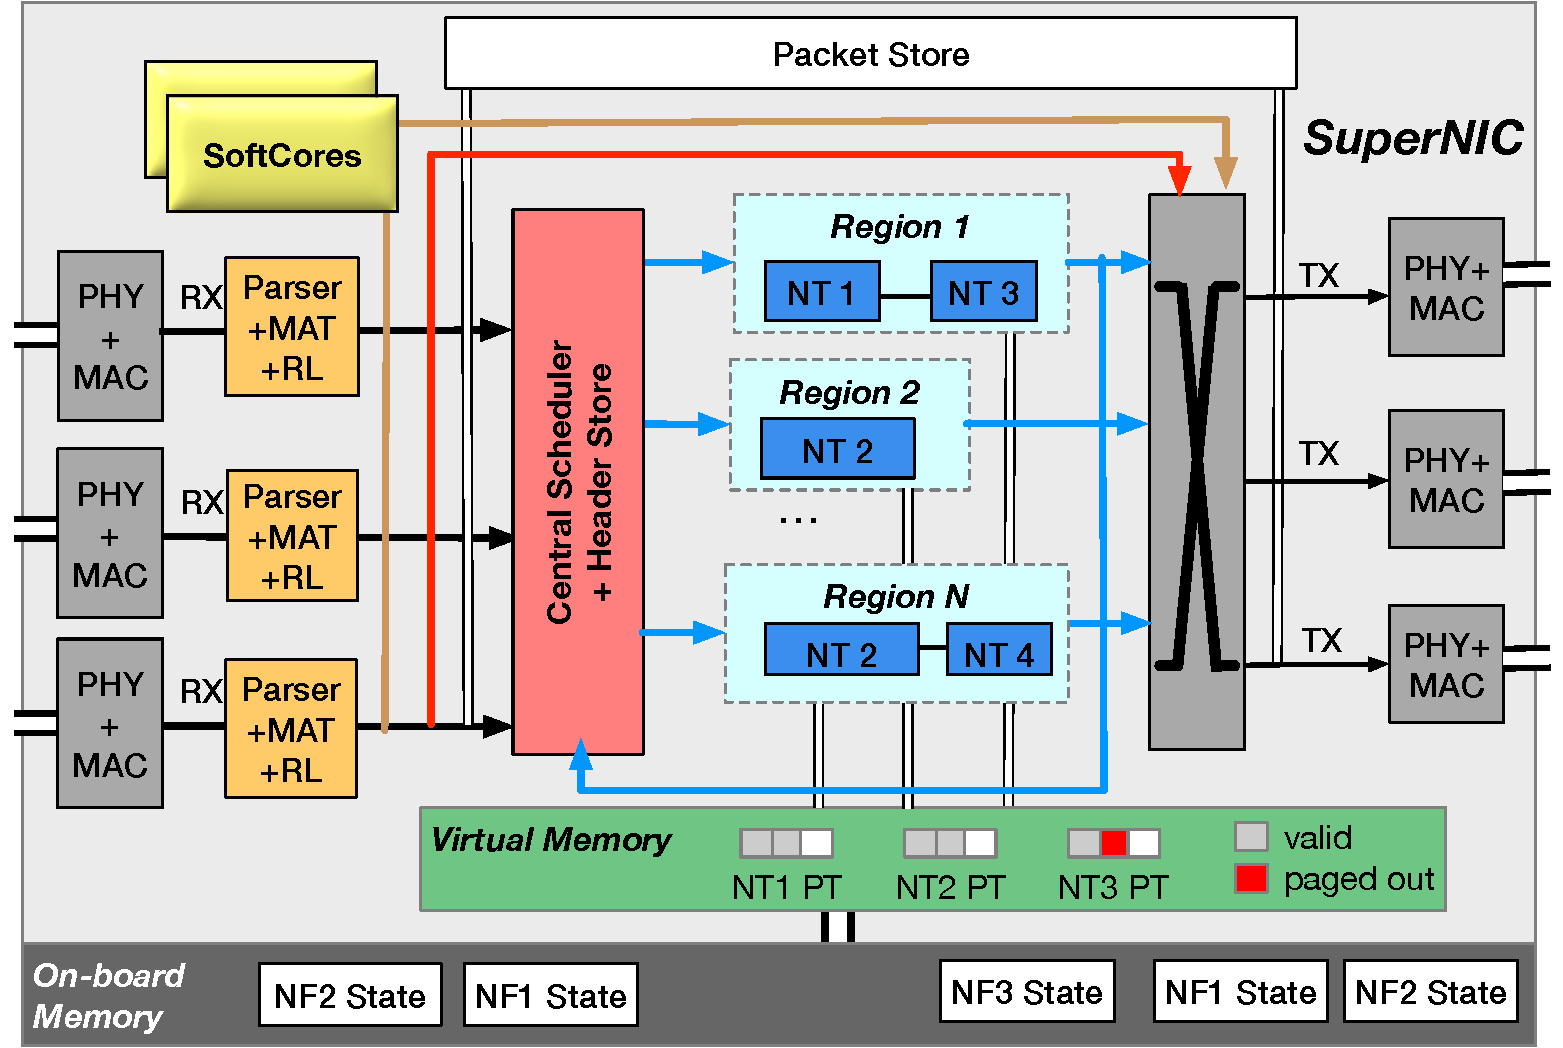
\includegraphics[width=\textwidth]{snic/Figures/board.pdf}}
\mycaption{fig-snic-board}{\snic\ On-Board Design.}
{
RL: Rate Limiter. PT: Page Table
}
\end{center}
\end{figure*}
}
{
\begin{figure*}[th]
\begin{center}
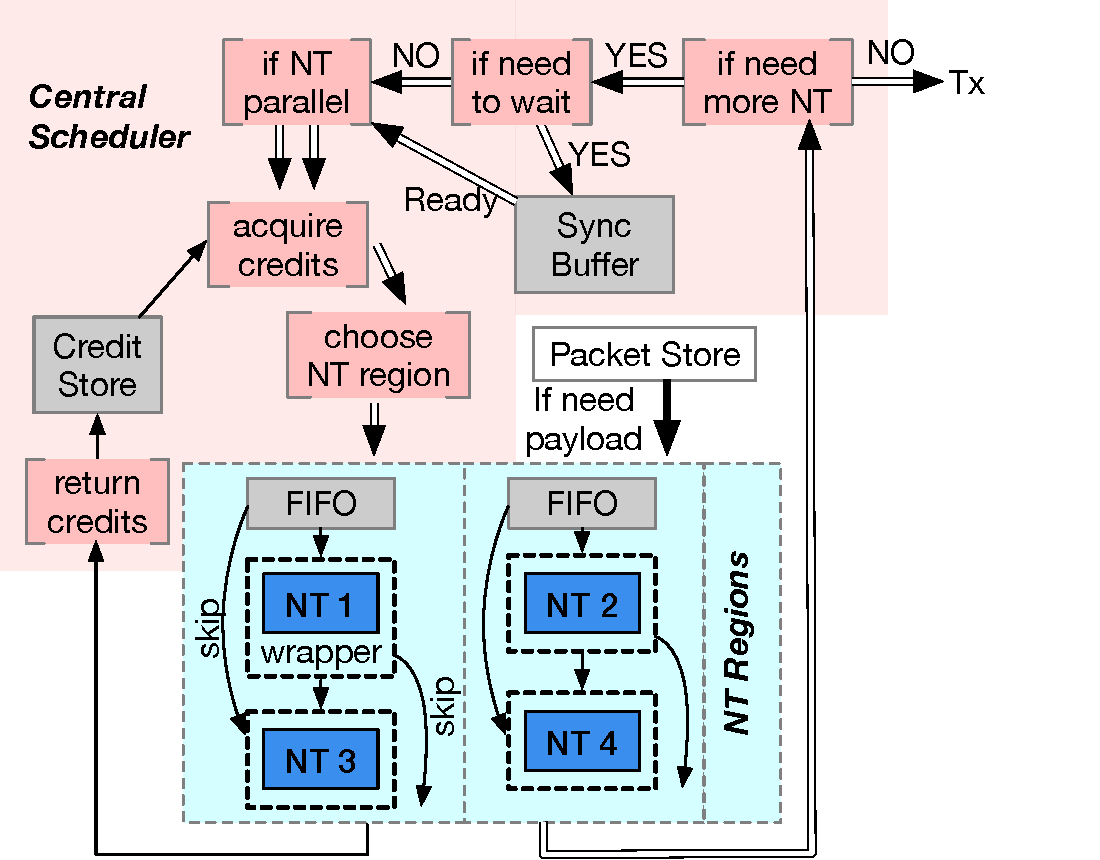
\includegraphics[width=0.9\textwidth]{snic/Figures/scheduler.pdf}
\mycaption{fig-sched}{\snic\ Packet Scheduler and \nt\ Region Design.}
{
Double arrows, single arrows, and thick arrows represent packet headers, credits, and packet payload.
}
\end{center}
\end{figure*}
}

Traditional server SmartNICs have plenty of hardware resources when hosting network functions for applications running on the local server~\cite{SmartNIC-nsdi18,Caulfield-2018}.
In contrast, \snic{} is anticipated to often be fully occupied or even over-committed, as it needs to host \nt{}s from more tenants with limited hardware resources to save costs.
Thus, a key and unique challenge in designing \snic{}s is space- and performance-efficient consolidation in a multi-tenant environment.
Moreover, \snic\ faces a more dynamic environment where not only the load of an application but also applications themselves could change from time to time.
Thus, unlike traditional SmartNICs that focus on packet processing and packet scheduling, \snic\ also needs to schedule \nt{}s efficiently.
%, and both types of scheduling needs to accommodate to a dynamic, multi-tenant environment.
%be more scalable and more flexible.
This section first goes over the high-level architecture of \snic, then discusses our mechanisms for efficient packet and \nt\ scheduling, followed by the discussion of our scheduling and fairness policies, and ends with a description of \snic's virtual memory system.
%We handle the former with SoftCores and the latter with hardware.
%An \snic\ has three major tasks: packet processing, packet scheduling, and \nt\ scheduling.
%overall approach \fixme{TODO if have space}  

\subsection{Board Architecture and Packet Flow}

We design the \snic\ board to simultaneously achieve several critical goals:
\textbf{G1)} parsing/de-parsing and scheduling packets at line rate;
\textbf{G2)} high-throughput, low-latency execution of \nt\ DAGs;
\textbf{G3)} safe and fair sharing of all on-board resources;
\textbf{G4)} quick adaptation to traffic load and workload changes;
\textbf{G5)} good scalability to handle many concurrent workloads and \nt{}s;
\textbf{G6)} flexible configuration and adjustment of control-plane policies;
and \textbf{G7)} efficient usage of on-board hardware resources.
%using most of the on-board hardware resources for application \nt{}s.
Figure~\ref{fig-snic-board} illustrates the high-level architecture of the \snic\ board.

\snic's data plane consists of reconfigurable hardware (\eg, FPGA) for running user \nt{}s (blue parts in Figure~\ref{fig-snic-board})
and a small amount of non-reconfigurable hardware (ASIC) for non-user functionalities, similar to the ``shell'' or ``OS'' concept~\cite{Catapult-v2,Amazon-F1,amorphos-osdi18,coyote-osdi20}.
We choose a hardware-based data-plane design because \nt{}s like transports demand high-speed, parallel processing, and a fully reconfigurable hardware allows the maximum flexibility in \nt\ hardware designs.
Many of our design ideas can potentially be applied to other types of hardware and software \nt\ implementations, such as PISA pipelines and ARM cores.
%In our prototype, 90\% space of the \snic\ chip is dedicated for \nt{}s (\textbf{G7}).

We divide the \nt\ area into {\em region}s, each of which could be individually reprogrammed to run different \nt{}s.
Different \nt\ regions can be executed in parallel.

The control plane runs as software on a small set of general-purpose cores (SoftCores for short) (\eg, a small ARM-based SoC). 
To achieve the performance that the data plane requires and the flexibility that the control plane needs, we cleanly separate these two planes.
The data plane handles all packet processing on ASIC and FPGA (\textbf{G1}).
The control plane is responsible for setting up policies and scheduling \nt{}s and is handled by the SoftCores (\textbf{G6}).
In our prototype, we built everything on FPGA. 


When a packet arrives at an RX port, it goes through a standard physical and reliable link layer.
Then our parser parses the packet's header and uses a Match-and-Action Table (MAT) to decide where to route the packet next.
The parser also performs rate limiting for multi-tenancy fairness (\S\ref{sec:snic:policy}).
The parser creates a packet descriptor for each packet and attaches it to its header. The descriptor contains fields for storing metadata, such as an \nt\ DAG UID and the address of the payload in the packet store. 
The SoftCores determine and install rules in the MAT, which include three cases for routing packets to the next step.
%There are three cases.
First, if a packet specifies no \nt\ information or is supposed to be handled by another \snic\ (\S\ref{sec:snic:dist}), the \snic\ will only perform simple switching functionality and send it to the corresponding TX port (red line).
Second, if a packet specifies the operation type \texttt{CTRL}, it will be routed to the SoftCores (orange line). These packets are for control tasks like adding or removing \nt{}s, adding \nt\ DAGs (\S\ref{sec:snic:ntsched}), and control messages sent from other \snic{}s (\S\ref{sec:snic:dist}).

Finally, all the remaining packets need to be processed on the \snic, which is the common case.
Their payloads are sent to the {\em packet store}, and their headers go to a central scheduler (black arrows). 
The scheduler determines when and which \nt\ chain(s) will serve a packet and sends the packet to the corresponding region(s) for execution (blue arrows).
If an \nt\ needs the payload for processing, the payload is fetched from the packet store and sent to the \nt.
During the execution, an \nt\ could access the on-board memory through a virtual memory interface, in addition to accessing on-chip memory.
After an \nt\ chain finishes, if there are more \nt{}s to be executed, the packet is sent back to the scheduler to begin another round of scheduling and execution.
When all \nt{}s are done, the packet is sent to the corresponding TX port.
%, which uses an arbiter to guarantee bandwidth fairness across applications.


\subsection{Packet Scheduling Mechanism}
\label{sec:snic:packetsched}

We now discuss the design of \snic's packet scheduling mechanism. Figure~\ref{fig-sched} illustrates the overall flow of \snic's packet scheduling and execution.
%To efficiently execute such complex \nt\ DAGs, we first propose the concept of {\em \nt\ chain}, which allows one packet to be processed by a chain of \nt{}s without the need to go through the scheduler multiple times.
%Second, we build a flexible run-time system that supports both {\em \nt-level parallelism} (running different \nt{}s in parallel) and {\em instance-level parallelism} (running multiple instances of the same \nt{}s in parallel) in hardware.
%Existing hardware-based network function systems like Click~\cite{clicknp-sigcomm16}, E2~\cite{e2-sosp15}, and PANIC~\cite{panic-osdi20} focus on scheduling a single NF or a simple sequence of NFs with instance-level parallelism.
%\snic\ provides all three types of scheduling: \nt\ chaining, \nt-level parallelism, and instance-level parallelism, and in a scalable, efficient way.
%Doing so achieves high-throughput, low-latency \nt\ DAG execution (\textbf{G2}), quick adaptation to traffic load changes (\textbf{G4}), and fast and scalable scheduling (\textbf{G5}).

\bolditpara{\nt-chain-based FPGA architecture and scheduling.}
%Today's network systems are seeing increasing amounts of network functions that can be executed as a DAG (\eg, previous work found 53.8\% NF pairs can run in parallel~\cite{NFP-sigcomm17}).
As \snic\ enables more types of endpoints and workloads to offload their network tasks, the number of \nt{}s and their execution flows will become even more complex, which could impact both the complexity of board design and the performance of packet scheduling.
Our idea to confront these challenges is to execute as many \nt{}s as possible in one go, by chaining \nt{}s together.
%There can be different ways to split an \nt\ DAG can 
We put chained \nt{}s (called an {\em \nt\ chain}) in one \nt\ region (\eg, \nt{}1$\xrightarrow[]{}$\nt{}3 and \nt{}2$\xrightarrow[]{}$\nt{}4 in Figure~\ref{fig-snic-board}).
%A packet that uses a chain goes through all the \nt{}s in the chain without the need to involve the scheduler in between.
Instead of connecting each \nt\ to a central scheduler (as what PANIC~\cite{panic-osdi20} does), we connect each region to the scheduler.
Doing so allows us to use a much smaller crossbar between the \nt\ regions and the central scheduler, thereby reducing hardware complexity and area cost (\textbf{G7}).

Furthermore, we leverage \nt\ chains to reduce the scheduling overhead and improve the scalability of the central scheduler.
Our idea is to {\em reserve} credits for an {\em entire} \nt\ chain as much as possible and then execute the chain as a whole; only when that is not possible, we fall back to a mechanism that may involve the scheduler in the middle of a chain. 
Doing so reduces the need for a packet to go through the scheduler after every \nt, thereby improving both the packet's processing latency and the central scheduler's scalability (\textbf{G5}).

On top of the fixed chain design, we propose an optimization to enable efficient \nt\ time sharing across multiple users and to accommodate cases where some packets of an application only access a part of a chain (\textbf{G4}, \textbf{G6}).
Our idea is to support the {\em skipping} of arbitrary \nt(s) in a chain.
For example, a user can access \nt{}1 and \nt{}4 by first skipping \nt{}3 in Region-1 and then skipping \nt{}2 in Region-2 in Figure~\ref{fig-sched}.


\noindent{\ul{\textbf{Scheduling packets with \nt-level and instance-level parallelism.}}}~~
At an \snic, different regions run in parallel.
We exploit two types of parallelism by controlling what \nt{}s to put in parallel regions.
The first type concurrently executes {\em different packets} at multiple instances of the {\em same \nt\ chain} (what we call {\em instance-level parallelism}).
We automatically create more/less instances of an \nt\ chain based on load and send different packets in a round-robin way to the parallel instances.
We will discuss our \nt\ autoscaling policy in \ref{sec:snic:policy}.


The second type concurrently executes the {\em same packet} at multiple {\em different \nt{}s} (what we call {\em \nt-level parallelism}).
We infer what \nt{}s can run in parallel in an \nt\ DAG (\eg, in Figure~\ref{fig-nt-example}, \nt{}1 and \nt{}2 can run in parallel with \nt{}3 for user1).
We expect a fair amount of opportunities to explore \nt-level parallelism, as previous work found that 53.8\% NF pairs can run in parallel~\cite{NFP-sigcomm17}.
To execute a packet at several \nt{}s concurrently, the scheduler makes copies of the packet header and sends them to these \nt{}s concurrently. To obey the order of \nt{}s that users specify, we maintain a {\em synchronization buffer} to store packet headers after they return from an \nt{}'s execution and before they could go to the next stage of \nt{}s (Figure~\ref{fig-sched}).

{
\begin{figure*}
\begin{center}
\centerline{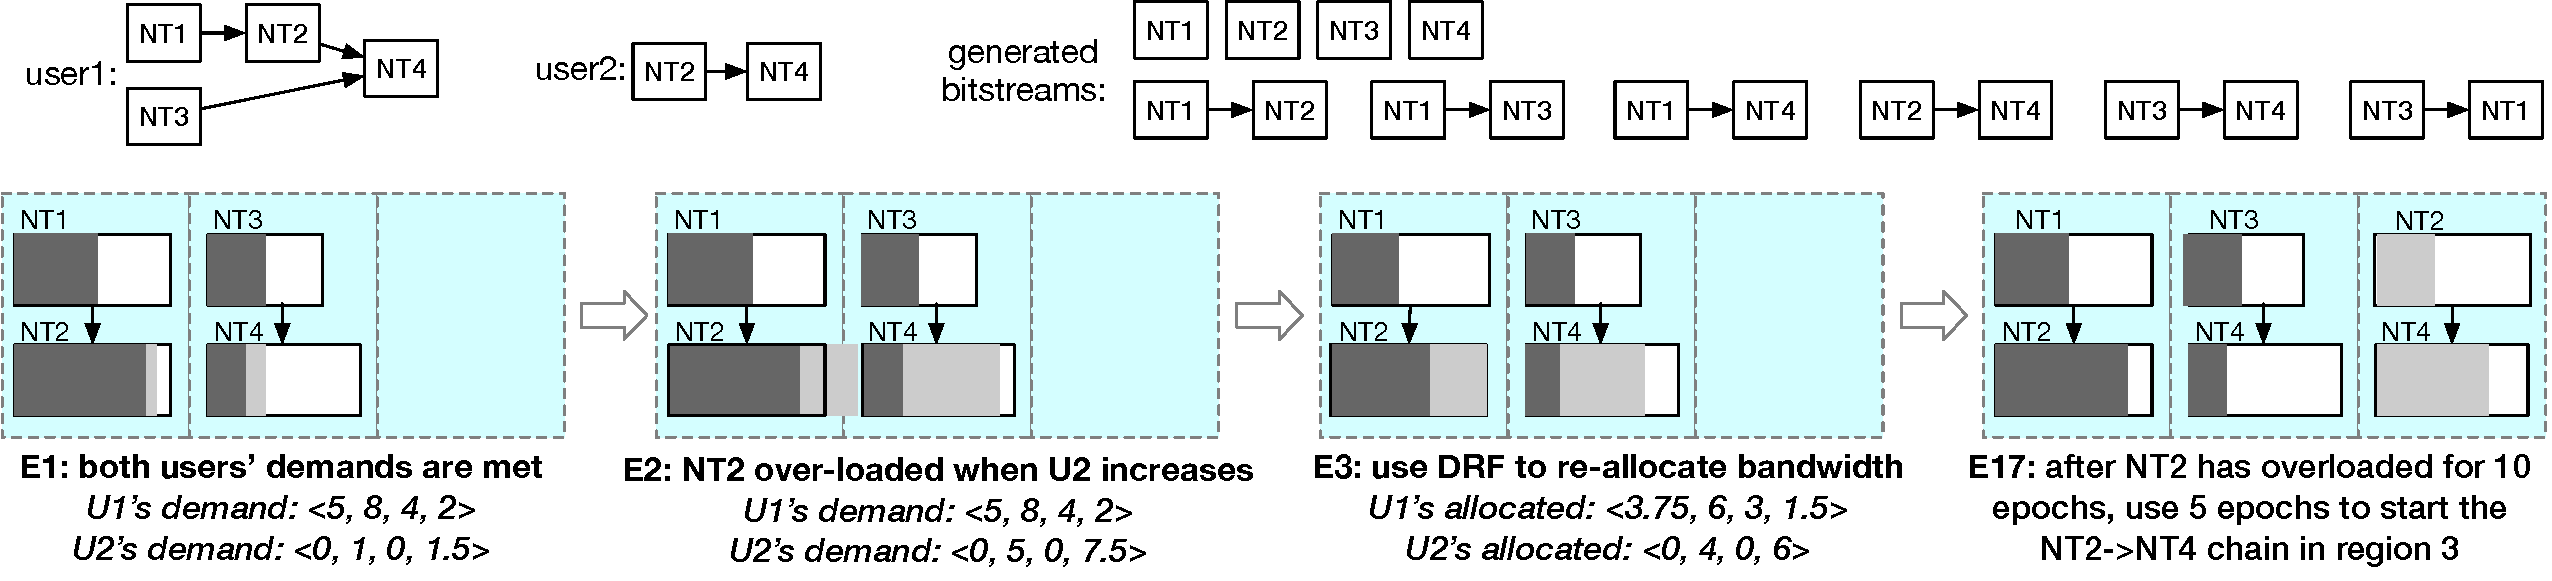
\includegraphics[width=0.9\textwidth]{Figures/nt-example.pdf}}
\vspace{-0.1in}
\mycaption{fig-nt-example}{An Example of \nt\ chaining and scheduling.}
{
Top: user1 and user2's \nt\ DAGs and \snic's generated bitstreams for them.
Bottom: timeline of \nt\ bandwidth allocation change.
Dark grey and light grey represent user1 and user2's load.
The launched chains are \nt{}1$\xrightarrow[]{}$\nt{}2 and \nt{}3$\xrightarrow[]{}$\nt{}4,
with \nt{}2 and \nt{}4 being shared by the two users.
The maximum throughput of NT1, NT2, and NT4 are 10 units each, and NT3's is 7 units.
NT2 is the dominant resource for user1, and NT4 is the dominant for user2.
}
\end{center}
\vspace{-0.2in}
\end{figure*}
}


\subsection{\nt\ (De-)Launching Mechanism}
\label{sec:snic:ntsched}
\snic's SoftCore handles \nt\ deployment, launch, and scheduling tasks, as a part of the control path.
A new challenge specific to \snic\ comes from the need to do more frequent \nt\ reconfigurations than traditional programmable network devices.
To enable more consolidation, we allow multiple \nt{}s to {\em time share} an FPGA space, and we auto-scale \nt{}s.
Both these cases involve the slow FPGA PR process.
We propose a set of new mechanisms and policies to reduce or hide the PR costs.
We now discuss the mechanisms and defer the policy discussions to \S\ref{sec:snic:policy}.

\bolditpara{\nt\ deployment.}~~
Users deploy \nt{}s to the \snic\ platform ahead of time as FPGA netlists (which can be thought of as Intermediate Representations in software).
When receiving newly deployed \nt{} netlists for an application, we first generate a set of FPGA bitstreams (which can be thought of as executable binaries in software).
We enumerate all possible combinations of \nt{}s under user-specified \nt\ DAG ordering requirements when generating bitstreams. 
This is because bitstream generation is a slow process that usually takes a few hours or even longer. 
Generating more bitstreams at deployment time gives the \snic\ more flexibility to choose different \nt\ combinations at the run time. 
Figure~\ref{fig-nt-example} shows an example of generated bitstreams based on two DAGs of two users.
%\noteyiying{delete the following sentence if need more space}
%We do not generate bitstreams for three-\nt{} chains in this example, as that exceeds what a region can hold.
%For example, with three \nt{}s where the user specifies the first two to fan in to the third, we generate bitstreams for \nt{}1, \nt{}2, \nt{}3, \nt{}1$\xrightarrow{}$\nt{}2, \nt{}2$\xrightarrow{}$\nt{}1, \nt{}1$\xrightarrow{}$\nt{}3, \nt{}2$\xrightarrow{}$\nt{}3, \nt{}1$\xrightarrow{}$\nt{}2$\xrightarrow{}$\nt{}3, and \nt{}2$\xrightarrow{}$\nt{}1$\xrightarrow{}$\nt{}3.
We store pre-generated bitstreams in the \snic{}'s on-board memory; each bitstream is small, normally less than 5\MB.

When generating bitstreams, we attach a small \snic\ wrapper to each \nt\ (Figure~\ref{fig-sched}).
%This module monitors the load of each \nt\ and \yiying{Will, what else is in the module?}
This wrapper is essential: it enables skipping an \nt\ in a chain (\S\ref{sec:snic:packetsched}), monitors the runtime load of the \nt\ (\S\ref{sec:snic:policy}), ensures signal integrity during PR, and provides a set of virtual interfaces for \nt{}s to access other board resources like on-board memory (\S\ref{sec:snic:memory}).

\bolditpara{\nt\ chain launching.}~~
We start a new \nt\ chain when an application is deployed (pre-launch), when the chain is first accessed by a packet in an application (on-demand), or when we scale out an existing \nt\ chain. For the first and third cases, we start the new \nt\ only when there is a free region (see \S\ref{sec:snic:policy} for detail).
%The SoftCore picks a free region to launch the chain. 
For the on-demand launching case, when all regions are full, we still need to launch the new chain to be able to serve the application. In this case, we need to de-schedule a current \nt\ chain to launch the new chain (see \S\ref{sec:snic:policy} for how we pick the region).

The \snic\ SoftCore handles this context switching with a {\em stop-and-launch} process.
Specifically, the SoftCore sends a signal to the current \nt{}s to let them ``stop''.
These \nt{}s then store their states in on-board memory to prepare for the stop.
At the same time, the SoftCore informs the scheduler to stop accepting new packets. 
The scheduler will buffer packets received after this point.
After the above {\em stop step}s finish, the SoftCore reads the new bitstream from the on-board memory via DMA and starts the FPGA PR process ({\em launch}).
This process is the slowest step, as the maximum reported achievable PR throughput is around 800\,MB/s~\cite{coyote-osdi20}, or about 5\,\ms\ for our default region size.
Afterwards, the newly launched chain can start serving packets, and it will first serve previously buffered packets, if any.

%\boldpara{Swap and victim region.}~~
%A unique and new challenge in scheduling \nt{}s in FPGA is that unlike software, the \nt\ region reconfiguration process as described above is slow. 
%We tackle this challenge from both the mechanism and policy perspectives.
%We now discuss our ideas in mechanisms.

To reduce the overhead caused by \nt\ reconfiguration, we use a technique similar to the traditional victim cache design. We keep a de-scheduled \nt\ chain in a region around for a while unless the region is needed to launch a new chain. If the de-scheduled \nt\ chain is accessed again during this time, we can directly use it in that region, reducing the need to do PR at that time.

%we always leave one or few regions empty; we call them {\em swap region}s.
%To start a new chain, the SoftCore directly launches it in one swap region and start processing new packets with it.
%In the background, the SoftCore de-schedule an \nt\ chain by performing the {\em stop} step as illustrated above to create one more swap region.
%This swap region approach allows us to reduce the reconfiguration time to only the {\em launch} time. 

%Our second idea is inspired by victim cache in the traditional CPU architecture. 
%When de-scheduling an \nt\ chain, instead of clear the region, we leave it as is and tag it as a special {\em victim swap region}.
%If a swap region is needed to launch a new chain, this region can be picked.
%Otherwise, before it's picked, if packets access this chain again, they can directly use the region.
%If the chain's load is increased to be more than another chain's load, this other chain's region will be marked as the victim region, and the original victim region becomes a normal region.
%Our victim region approach avoids the overhead of de-scheduling and launching an \nt\ chain when there's only a short period of low load.

\subsection{Packet and \nt\ Scheduling Policy}
\label{sec:snic:policy}

We now discuss our packet and \nt\ scheduling policies.
Figure~\ref{fig-nt-example} shows an example of how an \snic\ with three regions evolves as load changes.

\bolditpara{Overall \nt\ scheduling strategy.}~~
Our overall strategy is to avoid FPGA PR as much as possible and treat \nt\ context switching (\ie, replacing a current \nt\ chain with a new one through FPGA PR) as a last resort, since context switching prevents the old \nt\ from running altogether and could result in thrashing in the worst case. 

For on-demand \nt\ launching, we first check if the \nt\ is the same as any existing \nt{} on the \snic.
If so, and if the existing \nt{} still has available bandwidth, we time share the existing \nt\ with the new application. %(\circled{1}).
In this case, new traffic can be served immediately.
Otherwise, we check if there is a free region.
If so, we launch the \nt\ at this region, and new traffic can be served after FPGA PR finishes.
Otherwise, we reach out to the distributed \snic\ platform and check if any other \snic\ has the same \nt\ with available bandwidth or a free region. 
If so, we route traffic to that \snic\ (to be discussed in \S\ref{sec:snic:dist}).
Otherwise, we run the \nt\ at the endpoint if users provide the alternative way of executing it there.
%user an alternative way of launching the \nt, \eg, running in hardware or software at the endpoint.
If all of the above fail, we resort to context switching by picking the region that is least loaded and using stop-and-launch to start the \nt.

We also try to hide PR latency behind the performance-critical path as much as possible.
%This is because it is slow to switch contexts (involving reconfiguring \nt{}s) and the 
Specifically, when a new application is deployed, we check if any of its \nt{}s is missing on an \snic. If there are any and if there are free regions on the \snic\ for these \nt{}s, we {\em pre-launch} them at the free regions, instead of launching them {\em on-demand} when the first packet accesses the \nt{}s, as the latter would require waiting for the slow PR and slow down the first few packets. 
%These pre-launched \nt{}s are the first batch of victims we choose to de-schedule if free regions are needed for other \nt{}s.

\bolditpara{\nt\ auto-scaling.}~~
To adapt to load changes, \snic\ automatically scales out/down instances of the same \nt\ (instance-level parallelism) (\textbf{G2, G4}).
Specifically, we use our per-\nt\ monitoring module to identify bottleneck \nt{}s and the load that they are expected to handle.
If there are free regions, we add more instances of these \nt{}s by performing PR on the free regions.
When the load to an \nt\ reduces to what can be handled with one instance less, we stop one of its instances and migrate the traffic of the stopped instance to other running instances.
Since PR is slow, we should scale out/down an \nt\ only if there is a persistent load increase/decrease instead of just occasional load spikes.
To do so, we only scale out/down an \nt\ if the past \texttt{MONITOR\_PERIOD} time has overloaded/underloaded the \nt.
\texttt{MONITOR\_PERIOD} should be at least longer than the PR latency to avoid thrashing. Since our measured PR latency is 5\ms, we set \texttt{MONITOR\_PERIOD} to be 5\ms\ by default. 
After experimenting other length, we find this length to work the best with most real-world traffic~\cite{facebook-sigcomm15,Atikoglu12-SIGMETRICS}.
%\noteyiying{Update this after getting Will's new monitoring sensitivity results.}
%\texttt{HIGH\_LOAD} is a heuristic depending on workloads.
%Previous works have reported different traffic peak lengths~\cite{facebook-sigcomm15,facebook-sigmetrics12}, \eg, millisecond-level in the 2015 Facebook trace~\cite{facebook-sigcomm15}, for which we could set \texttt{HIGH\_LOAD} to \fixme{XXX}.

\bolditpara{Scheduling with fairness.}~~
As we target a multi-tenant environment, \snic\ needs to fairly allocate its resources to different applications (\textbf{G3}).
%On top of the above strategy, we seek fairness across applications.
Different from existing fairness solutions, we treat every \nt\ as a separate type of resource, in addition to ingress bandwidth, egress bandwidth, packet store, and on-board memory space.
This is because we support the time sharing of an \nt, and different \nt{}s can be shared by different sets of users. Our fairness policy follows Dominant Resource Fairness (DRF)~\cite{DRF}, where we identify the {\em dominant} resource type for each application and seek a fair share for each application's dominant type. We also support weighted DRF~\cite{DRF,beyond-DRF} for users with different priorities.

Instead of a user-supplied static resource demand vector used in traditional DRF systems, we use {\em dynamically monitored resource demands} as the target in the DRF algorithm.
Specifically, at each {\em epoch}, we use the ingress parser, egress de-parser, the central scheduler, and our virtual memory system to monitor the actual load demand before requests are dispatched to a particular type of resource.
For example, for each user, the central scheduler measures the rate of packets that should be sent next to an \nt\ before assigning credits; \ie, even if there is no credit for the \nt, we still capture the intended load it should handle.
Based on the measured load at every type of resource for an application, we determine the dominant type of resource and use DRF to allocate resources after considering all applications' measured load vectors.
At the end of every epoch, our DRF algorithm outputs a new vector of resource allocation for each application, which the next epoch will use.
Compared to static resource demand vectors, our run-time monitoring and dynamic resource vectors can promptly adapt to load changes to maximize resource utilization. % with a higher degree of consolidation.

%We rerun the DRF algorithm right after scaling out/down an \nt{}, since scaling essentially changes the ``cap'' of the \nt's resource amount.

Another novelty is in how we achieve the assigned allocation.
Instead of throttling an application's packets at each \nt\ and every type of resource to match the DRF allocation, we only control the application's ingress bandwidth allocation.
Our observation is that since each \nt's throughput for an application, its packet buffer space consumption, and egress bandwidth are all proportional to its ingress bandwidth, we could effectively control these allocations through the ingress bandwidth allocation.
Doing so avoids the complexity of throttling management at every type of resource.
Moreover, throttling traffic early on at the ingress ports helps reduce the load going to the central scheduler and the amount of payload going to the packet store.
Our current implementation controls ingress bandwidth through rate limiting.
Future work could also use other mechanisms like Weighted Fair Queuing.
The only resource that is not proportional to ingress bandwidth is on-board memory space.
We control it through our virtual memory system (\S\ref{sec:snic:memory}).

Finally, the length of an epoch, \texttt{EPOCH\_LEN}, is a configurable parameter.
At every epoch, we need to run the DRF algorithm and possibly change the bandwidth and memory allocation.
Thus, \texttt{EPOCH\_LEN} should be longer than the time taken to perform these operations (around 3\mus\ with our implementation).
%Our measured time is 3\mus\ for running the DRF algorithm, negligible for changing bandwidth, and 15-20\mus\ for swapping out a 2\MB\ page.
%Note that swapping out memory can be done in a lazy fashion and does not complete in an epoch.
Meanwhile, it is desirable to set a short \texttt{EPOCH\_LEN} to quickly adapt to load variations and to update rate allocations approximately once per average RTT~\cite{xcp-sigcomm02, rcp-sigcomm06}.
Thus, we set the default value of \texttt{EPOCH\_LEN} to 20\mus.

\subsection{Virtual Memory System}
\label{sec:snic:memory}
\snic's allow \nt{}s to use off-chip, on-board memory.
To isolate different applications' memory spaces and to allow the over-subscription of physical memory space in an \snic, we build a simple page-based virtual memory system.
\nt{}s access on-board memory via a virtual memory interface,
where each \nt\ has its own virtual address space.
Our virtual memory system translates virtual memory addresses into physical ones and checks access permissions with a single-level page table.
We use huge pages (2\MB\ size) to reduce the amount of on-chip memory to store the page table.
Physical pages are allocated on demand; when a virtual page is first accessed, \snic\ allocates a physical page from a free list.

We further support the over-subscription of an \snic's on-board memory, \ie, an \snic\ can allocate more virtual memory space than its physical memory space.
When the physical memory is full, adding more \nt\ would require shrinking memory already assigned to existing applications (\S\ref{sec:snic:ntsched}).
In this case, we reduce already assigned memory spaces by migrating memory pages to a remote \snic, \ie, swapping out pages.
To decide what pages to swap out, we first use the DRF algorithm to identify what \nt{}(s) should shrink their memory space. 
Within such an \nt, we pick the least recently accessed physical page to swap out.
Our virtual memory system tracks virtual memory accesses to capture per-page access frequency. 
It also transparently swaps in a page when it is accessed.
If no other \snic{} has free memory space when the \snic\ needs to grow its virtual memory space, we reject requests to add new \nt{}s or to enlarge existing \nt{}'s memory.
\section{Distributed SuperNIC}
\label{sec:dist}

The design discussion so far focused on a single \snic. To enable better consolidation and network as a service, we 
%When we use a single \snic\ to consolidate \nt{}s of its connected endpoints, the \snic\ needs to be provisioned with the aggregated peak load of these endpoints.
%To further reduce cost, we 
build a rack-scale distributed \snic\ platform that enables one \snic\ to use other \snic{}s' resources.
With this platform, a rack's \snic{}s can collectively provision for the maximum aggregated load of all the endpoints in the rack.

As discussed in \S\ref{sec:overview}, we support two types of \snic\ pool topology.
For the switch-attached topology, the ToR switch serves as the load balancer across different \snic{}s.
It also decides which \snic\ to launch a new instance of an \nt\ with the goal of balancing traffic and efficiently utilizing \snic\ hardware resources.
%Specifically, it chooses the \snic\ that has enough free regions and is lightly loaded to launch new instances of \nt\ chains.
%Afterwards, the switch simply directs incoming flows to the \snic{}s that contain their target \nt{}s.
Supporting the intermediate-pool topology where the ToR switch cannot perform the above tasks is more complex. Below we discuss our design for it.

%\boldpara{Distributed Control Plane.}~~
SoftCores on the \snic{}s in the intermediate pool form a distributed control plane. 
They communicate with each other to exchange metadata and cooperate in performing distributed tasks. % like \nt\ migration and memory swapping.
We choose this peer-to-peer design instead of a centralized one, because the latter requires another global manager and adds complexity and cost to the rack architecture. %\zac{I am not sure about this argument -- I have heard that other places (e.g. google) have used the centralized manager architecture because it's easier to build and deploy than P2P ones. I personally don't buy this argument either. Do you have stronger support?}
Every \snic\ collects its FPGA space, on-board memory, and port bandwidth consumption, and it periodically sends this information to all the other \snic{}s in the rack.
Each \snic\ thus has a global view of the rack and can redirect traffic to other \snic{}s if it is overloaded.
%make decisions like \nt\ migration independently.
To redirect traffic, the \snic's SoftCore sets a rule in the parser MAT to forward certain packets (\eg, ones to be processed by an \nt\ chain on another \snic) to the remote \snic.

%\notearvind{We could also talk about something more basic - if the same NT is loaded on many snics, we can balance the load across all instances and achieve good consolidation. Maybe that would be easier for reviewers to accept before we talk about NT migration.}

%\boldpara{\nt\ Migration.}~~
If an \snic\ is overloaded and no other \snic{}s currently have the \nt\ chain that needs to be launched, the \snic\ tries to launch the chain at another \snic.
Specifically, the \snic's SoftCore first identifies the set of \snic{}s in the same rack that have available resources to host the \nt\ chain.
Among them, it picks one that is closest in distance to it (\ie, fewest hops).
The \snic's SoftCore then sends the bitstreams of the \nt{} chain to this picked remote \snic, which launches the chain in one of its own free regions.
When the original \snic\ has a free region, it moves back the migrated \nt\ chain. 
%It does so by first launching the \nt\ chain locally, then removing the MAT tunneling rule, and finally instructing the remote \snic\ to remove its \nt\ chain.
If the \nt\ chain is stateful, then the SoftCore manages a state migration process after launching the \nt\ chain locally, by first pausing new traffic, then migrating the \nt's states (if any) from the remote \snic\ to the local \snic. %and finally removing the MAT rule.


\section{Case Studies}
\label{sec:snic:application}

We now present two use cases of \snic\ that we implemented, one for disaggregated memory and one for regular servers.

\subsection{Disaggregated Key-Value Store}
\label{sec:snic:kvstore}
We first demonstrate the usage of \snic\ in a disaggregated environment by adapting a
recent open-source FPGA-based disaggregated memory device called {\em Clio}~\cite{Clio}.
The original Clio device hosts standard physical and link layers, a Go-Back-N reliable transport, and a system that maps keys to physical addresses of the corresponding values.
Clients running at regular servers send key-value load/store/delete requests to Clio devices over the network.
When porting to \snic, we do not change the client-side or Clio's core key-value mapping functionality.

\bolditpara{Disaggregating transport.}~~
The Go-Back-N transport consumes a fair amount of on-chip resources %ß(5.8\% LUTs and 2.6\% BRAM of the Clio device and 
(roughly the same amount as Clio's core key-value functionality~\cite{clio-arxiv}).
%(mainly on-chip memory used to store states for retransmission). 
We move the Go-Back-N stack from multiple Clio devices to an \snic\ and consolidate them by handling the aggregated load.
After moving the Go-Back-N stack, we extend each Clio device's link layer to a reliable one (\S\ref{sec:snic:overview}).

\bolditpara{Disaggregating KV-store-specific functionalities.}~~
A unique opportunity that \snic\ offers is its centralized position when connecting a set of endpoints, which users could potentially use to more efficiently coordinate the endpoints.
We explore this opportunity by building a replication service and a caching service as two \nt{}s in the \snic.
%that connects the Clio devices.

For \textbf{replication}, the client sends a replicated write request with a replication degree $K$, which the \snic\ handles by replicating the data and sending them to $K$ Clio devices. 
In comparison, the original Clio client needs to send $K$ copies of data to $K$ Clio devices or send one copy to a primary device, which then sends copies to the secondary device(s).
The former increases the bandwidth consumption at the client side, and the latter increases end-to-end latency.

For \textbf{caching}, the \snic\ maintains recently written/read key-value pairs in a small buffer. It checks this cache on every read request. If there is a cache hit, the \snic\ directly returns the value to the client, avoiding the cost of accessing Clio devices. Our current implementation that uses simple FIFO replacement already yields good results. Future improvements like LRU could perform even better.

\subsection{Virtual Private Cloud}
\label{sec:snic:vpc}

Cloud vendors offer Virtual Private Cloud (VPC) for customers to have an isolated network environment where their traffic is not affected by others and where they can deploy their own network functions such as firewall, network address translation (NAT), and encryption.
Today's VPC functionalities are implemented either in software~\cite{andromeda-google-nsdi18,ovs-nsdi15,ovs-sigcomm21} or offloaded to specialized hardware at the server~\cite{vfp-nsdi17,SmartNIC-nsdi18,aws-nitro}.
As cloud workloads experience dynamic loads and do not always use all the network functions (\S\ref{sec:snic:motivation}), VPC functionalities are a good fit for offloading to \snic.
Our baseline here is regular servers running Open vSwitch (OVS) with three NFs, firewall, NAT, and AES encryption/decryption. %Both senders and receivers servers employ the same setting and are connected to a physical switch directly.
We connect \snic{}s to both sender and receiver servers and then offload these three NFs to each \snic\ as one \nt\ chain. 
\section{Evaluation Results}
\label{sec:snic:results}

We implemented \snic\ on the HiTech Global HTG-9200 board~\cite{htg9200}. 
Each board has nine 100\Gbps\ ports, 10\GB\ on-board memory, and a Xilinx VU9P chip with 2,586K LUTs and 43\MB\ BRAM.
We implemented most of \snic's data path in SpinalHDL~\cite{SpinalHDL} and \snic's control path in C (running in a MicroBlaze SoftCore~\cite{microblaze-xilinx} on the FPGA).
Most data path modules run at 250 MHz.
In total, \snic\ consists of 8.5K SLOC (excluding any \nt\ code).
The core \snic\ modules consume less than 5\% resources of the Xilinx VU9P chip, leaving most of it for \nt{}s (see Appendix for full report).
To put it in perspective, the Go-back-N reliable transport we implement consumes 1.3\% LUTs and 0.4\% BRAM.

\bolditpara{Environment.}~~ 
We perform both cycle-accurate simulation (with Verilator~\cite{verilator-site}) and real end-to-end deployment.
Our deployment testbed is a rack with a 32-port 100\Gbps\ Ethernet switch, two HTG-9200 boards acting as two \snic{}s, eight Dell PowerEdge
R740 servers, each equipped with a Xeon Gold 5128 CPU and an NVidia 100\Gbps\ ConnectX-4 NIC, and two Xilinx 10\Gbps\ ZCU106 boards running as Clio~\cite{clio-arxiv} disaggregated memory devices.
Each \snic\ uses one port to connect to the ToR switch and one port to connect to the other \snic.
Depending on different evaluation settings, an \snic{}'s downlinks connect to two servers or two Clio devices.

{
\begin{figure*}[th]
\begin{center}
\centerline{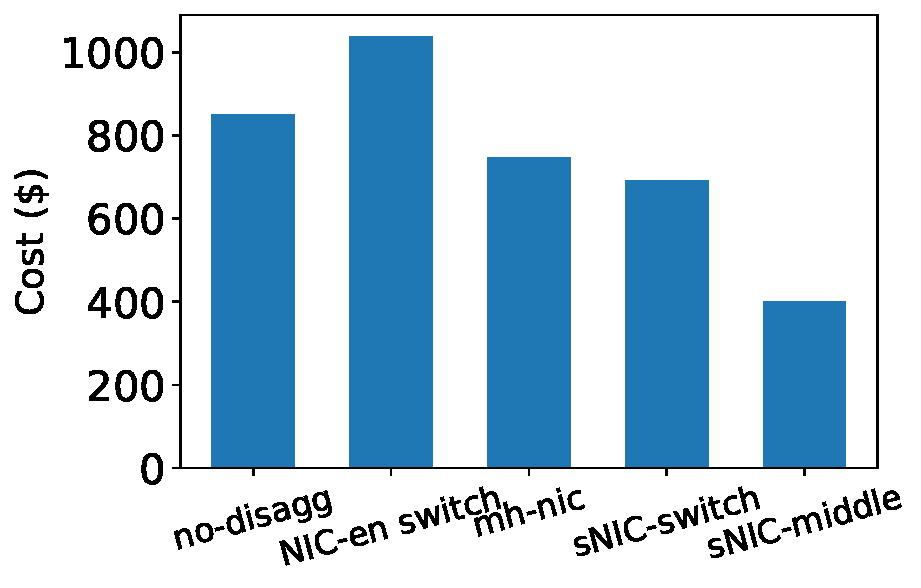
\includegraphics[width=0.5\textwidth]{snic/Figures/fig-single-rack-capex-perDevCost.pdf}}
\mycaption{fig-rack-capex}{Per-Endpoint CapEx.}
{
A rack's network cost divided by endpoint count. 
}
\end{center}
\end{figure*}
}
{
\begin{figure*}[h]
\begin{center}
\centerline{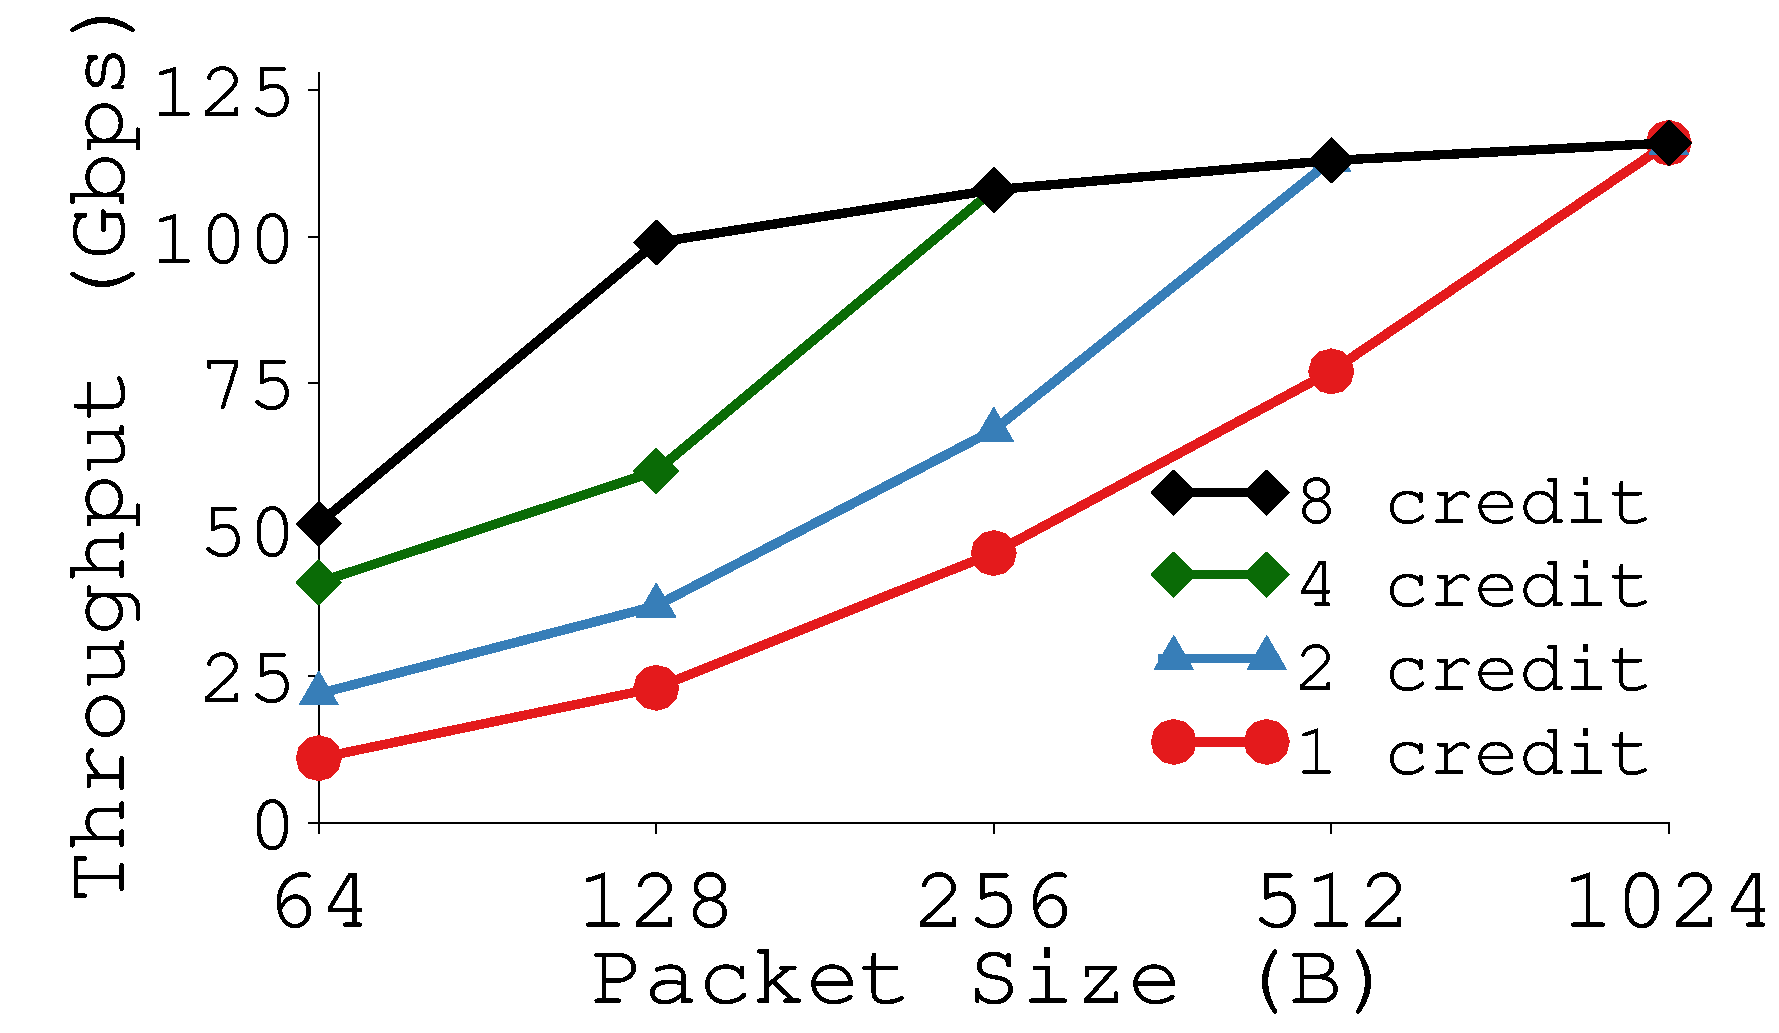
\includegraphics[width=0.5\textwidth]{snic/Figures/g_plot_credit.pdf}}
\mycaption{fig-credit}{Throughput with different credits.}
{
}
\end{center}
\end{figure*}
}
{
\begin{figure*}[h]
\begin{center}
\centerline{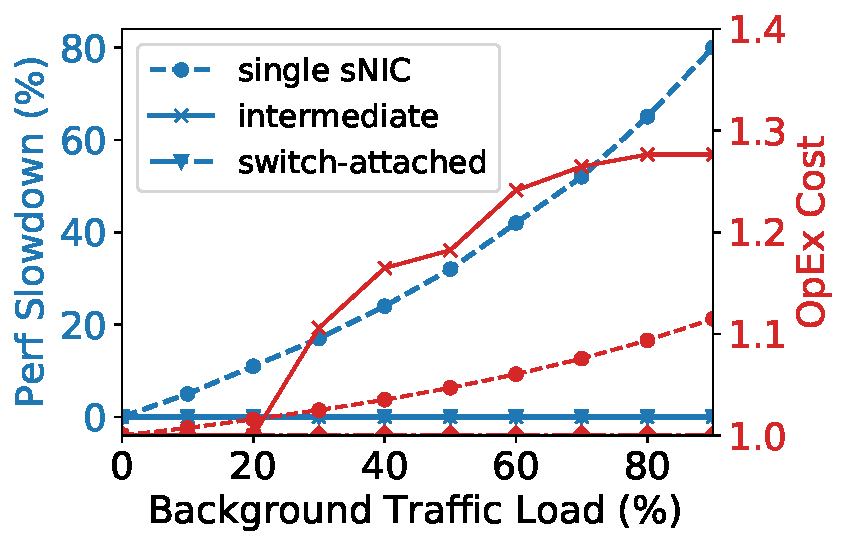
\includegraphics[width=0.5\textwidth]{snic/Figures/fig-dist-nic-load-increase.pdf}}
\mycaption{fig-sim-dist-nic}{Distributed \snic{}.}
{
}
\end{center}
\end{figure*}
}
{
\begin{figure*}[h]
\begin{center}
\centerline{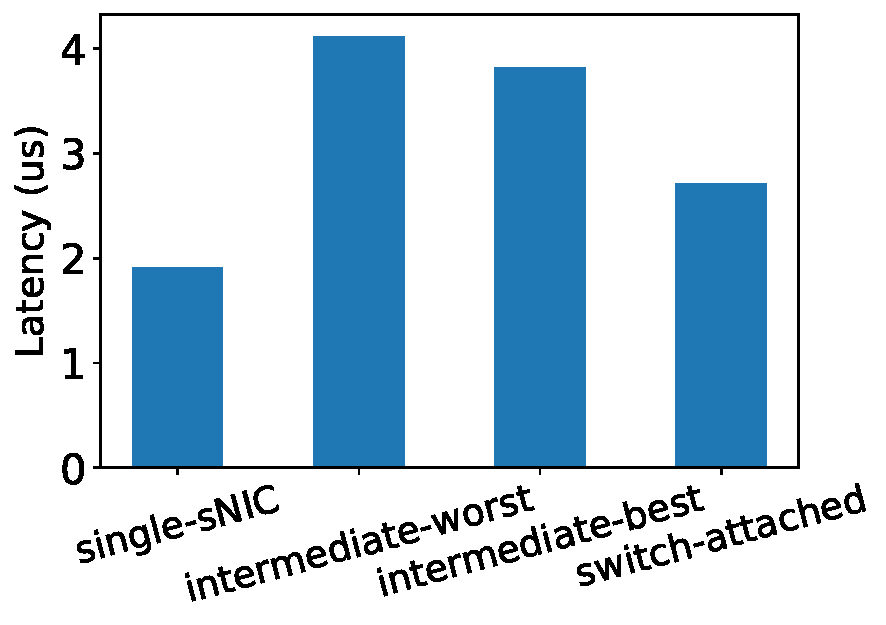
\includegraphics[width=0.5\textwidth]{snic/Figures/fig-dist-nic-latency.pdf}}
\mycaption{fig-topology-cmp}{Topology Comparison.}
{
}
\end{center}
\end{figure*}
}

\subsection{Overall Performance and Costs}
\label{sec:snic:eval-overview}

\bolditpara{CapEx cost saving.}~~
We compare the CapEx cost of \snic's two architectures with no network disaggregation, traditional multi-host NIC, and traditional NIC-enhanced switches.
All calculations are based on a single rack and include 1) endpoint NICs, 2) cables between endpoints, \snic{}s, and the ToR switch, 3) the ToR switch, and 4) cost of \snic{}s or multi-host NICs.
We use market price when calculating the price of regular endpoint NICs and cables.
With \snic, the endpoint NICs can be shrunken down to physical and link layers (based on our prototype estimation, it is roughly 20\% of the original NIC cost of \$500), and the cables connecting endpoints and \snic{}s in the middle-layer-pool architecture can be shortened (roughly 60\% of the original cable cost of \$100~\cite{RAIL-NSDI}).
We estimate the ToR-switch cost based on the number of ports it needs to support and a constant per-port cost of \$250~\cite{fs-64port-switch}.

To estimate the cost of an \snic, we separate the non-\nt\ parts and the \nt\ regions. The former has a constant hardware cost, while the latter can be provisioned to the peak of aggregated traffic and \nt\ usages, both of which are workload dependent. We use the peak-of-sum to sum-of-peak ratios obtained from the Facebook traces (\S\ref{sec:snic:benefits}). Today's multi-host NIC and NIC-enhanced switches do not consolidate traffic, and we assume that they will be provisioned for the sum-of-peak. See Appendix for detailed calculation. 

Figure~\ref{fig-rack-capex} plots the per-endpoint dollar CapEx cost. Overall, \snic\ achieves \textbf{52\% and 18\% CapEx savings} for the middle-layer and switch-attached pool architecture compared to no disaggregation.
Multi-host NIC and NIC-enhanced switches both have higher CapEx costs than \snic, because of its high provisioning without auto-scaling. The NIC-enhanced switches are even more costly than traditional racks mainly because of the added switch ports and NICs.

\bolditpara{OpEx saving and single-\snic\ performance.}~~
We compare a single \snic\ connecting four endpoints with the baseline of no disaggregation when these endpoints each run its \nt{}s on its own SmartNIC.
We generate workloads for each endpoint based on the Facebook memcached dataset distributions~\cite{Atikoglu12-SIGMETRICS}.
For the per-endpoint SmartNIC, we statically allocate the hardware resources that can cover the peak load.
Overall, we found that \snic\ achieves \textbf{56\% OpEx saving}, because \snic\ dynamically scales the right amount of hardware resources for the aggregated load.
\snic\ only adds \textbf{only 4\% performance overhead} over the optimal performance that the baseline gets with maximum allocation.

%\bolditpara{Single \snic\ throughput.}~~
We then test the throughput a real \snic\ board can achieve with a dummy \nt.
These packets go through every functional module of the \snic, including the central scheduler and the packet store. 
We change the number of initial credits and packet size to evaluate their effect on throughput, as shown in Figure~\ref{fig-credit}.
These results demonstrate that our FPGA prototype of \snic\ could reach more than 100\Gbps\ throughput. 
With higher frequency, future ASIC implementation could reach even higher throughput.
%Similar to PANIC~\cite{panic-osdi20}, we find that having more initial credits achieves higher throughput, and 8 credits are enough for 100\Gbps\ network.

Next, we evaluate the latency overhead a real \snic\ board adds.  
It takes 1.3\mus\ for a packet to go through the entire sNIC data path. % (PHY, MAC, sNIC core, MAC, and PHY). 
Most of the latency is introduced by the third-party PHY and MAC modules, which could potentially be improved with real ASIC implementation and/or a PCIe link. 
The \snic\ core only takes 196\,ns.
Our scheduler achieves a small, fixed delay of 16 cycles, or 64\,ns with the FPGA frequency. 
%The synchronization buffer has an overhead of 4 cycles, or 16\,ns.
To put things into perspective, commodity switch's latency is around 0.8 to 1\mus.  

\bolditpara{Distributed \snic{}s.}~~
To understand the effect of distributed \snic\ pool, we compare the two pool topology with a single \snic\ (no distributed support).
Figure~\ref{fig-sim-dist-nic} shows the performance and OpEx cost.
Here, we use the workload generated from the Facebook distribution as the foreground traffic and vary the load of the background traffic.
As background load increases, a single \snic\ gets more over-committed and its performance becomes worse.
With distributed \snic, we use an alternative \snic{} to handle the load, thus not impacting the foreground workload's performance. Note that the background workload's performance is not impacted either, as long as the entire \snic\ pool can handle both workloads' traffic. Furthermore, these workloads are throughput oriented, and we achieve max throughput with distributed \snic{}s.
As for OpEx, the intermediate-pool topology uses one \snic\ to redirect traffic to the other \snic.
As the passthrough traffic also consumes energy, its total OpEx increases as the total traffic increases.
The switch-attached topology does not have the redirecting overhead.
The single \snic\ also sees a higher OpEx as load increases because the workload runs longer and consumers more energy.

We then compare the two topologies of \snic\ pool. % and with no disaggregation. 
Figure~\ref{fig-topology-cmp} shows the latency comparison.
%As expected, no disaggregation achieves the best latency, as it does not need any additional network hops. 
The intermediate-pool topology where we connect the \snic{}s using a ring has a range of latency depending on whether the traffic only goes through the immediately connected \snic\ (single-\snic) or needs to be redirected to another \snic\ when the immediate \snic\ is overloaded. 
Because of the ring connection, this other \snic's distance to the immediately connected \snic\ determines the additional latency incurred (intermediate-best and worst).
In contrast, the switch-attached topology has a constant latency, even when one or multiple \snic{}s are overloaded. This is because the traffic always goes through the switch which directs it to the right \snic.

{
\begin{figure*}[th]
\begin{center}
\centerline{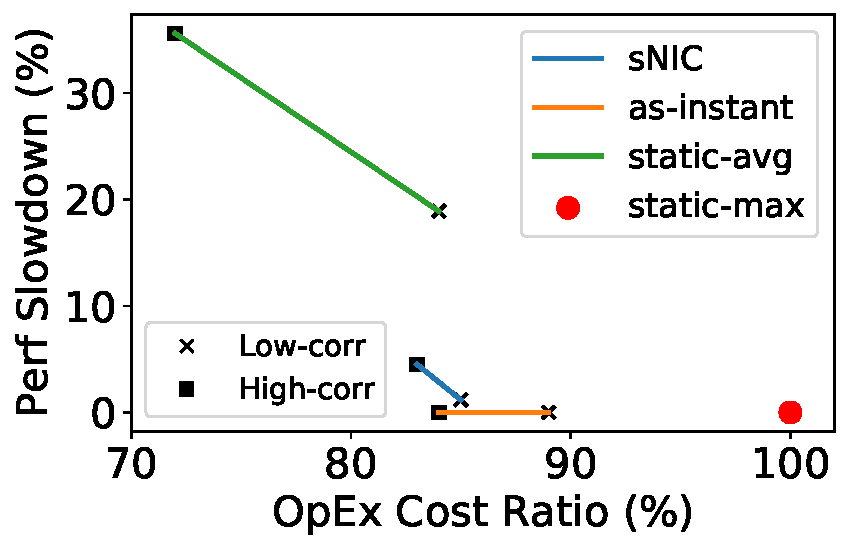
\includegraphics[width=0.5\textwidth]{snic/Figures/fig-conslid-overview-new.pdf}}
\mycaption{fig-sim-overview}{Performance and OpEx Overview.}
{
Lower is better for both axis.
}
\end{center}
\end{figure*}
}
{
\begin{figure*}[h]
\begin{center}
\centerline{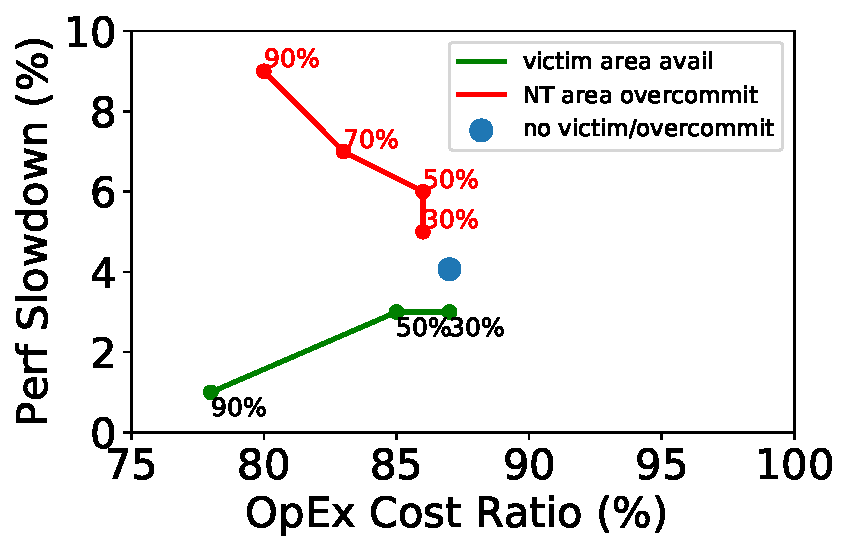
\includegraphics[width=0.5\textwidth]{snic/Figures/fig-single-snic-low-corr.pdf}}
\mycaption{fig-sim-single-snic}{Single \snic{} Sensitivity.}
{
Each lines is running a different set of experiments.
}
\end{center}
\end{figure*}
}
{
\begin{figure*}[h]
\begin{center}
\centerline{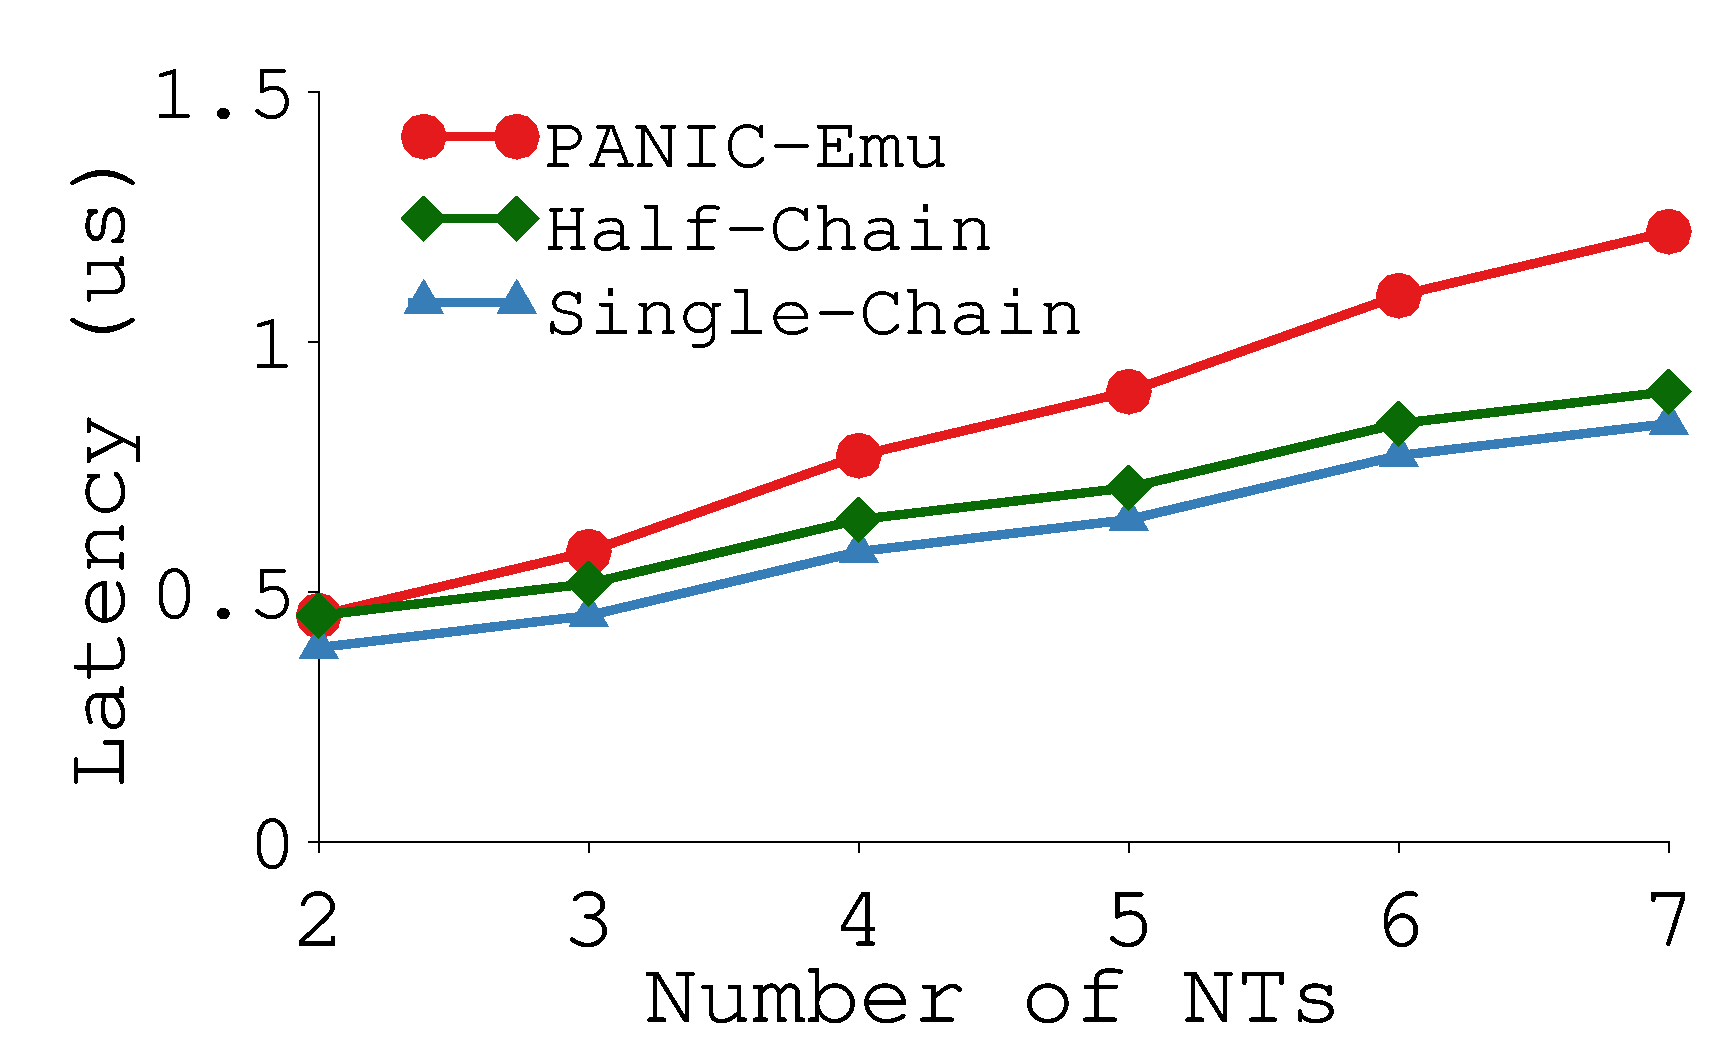
\includegraphics[width=0.5\textwidth]{snic/Figures/g_plot_nt_chain.pdf}}
\mycaption{fig-nt-chain}{\nt{} Chain.}
{
}
\end{center}
\end{figure*}
}
{
\begin{figure*}[h]
\begin{center}
\centerline{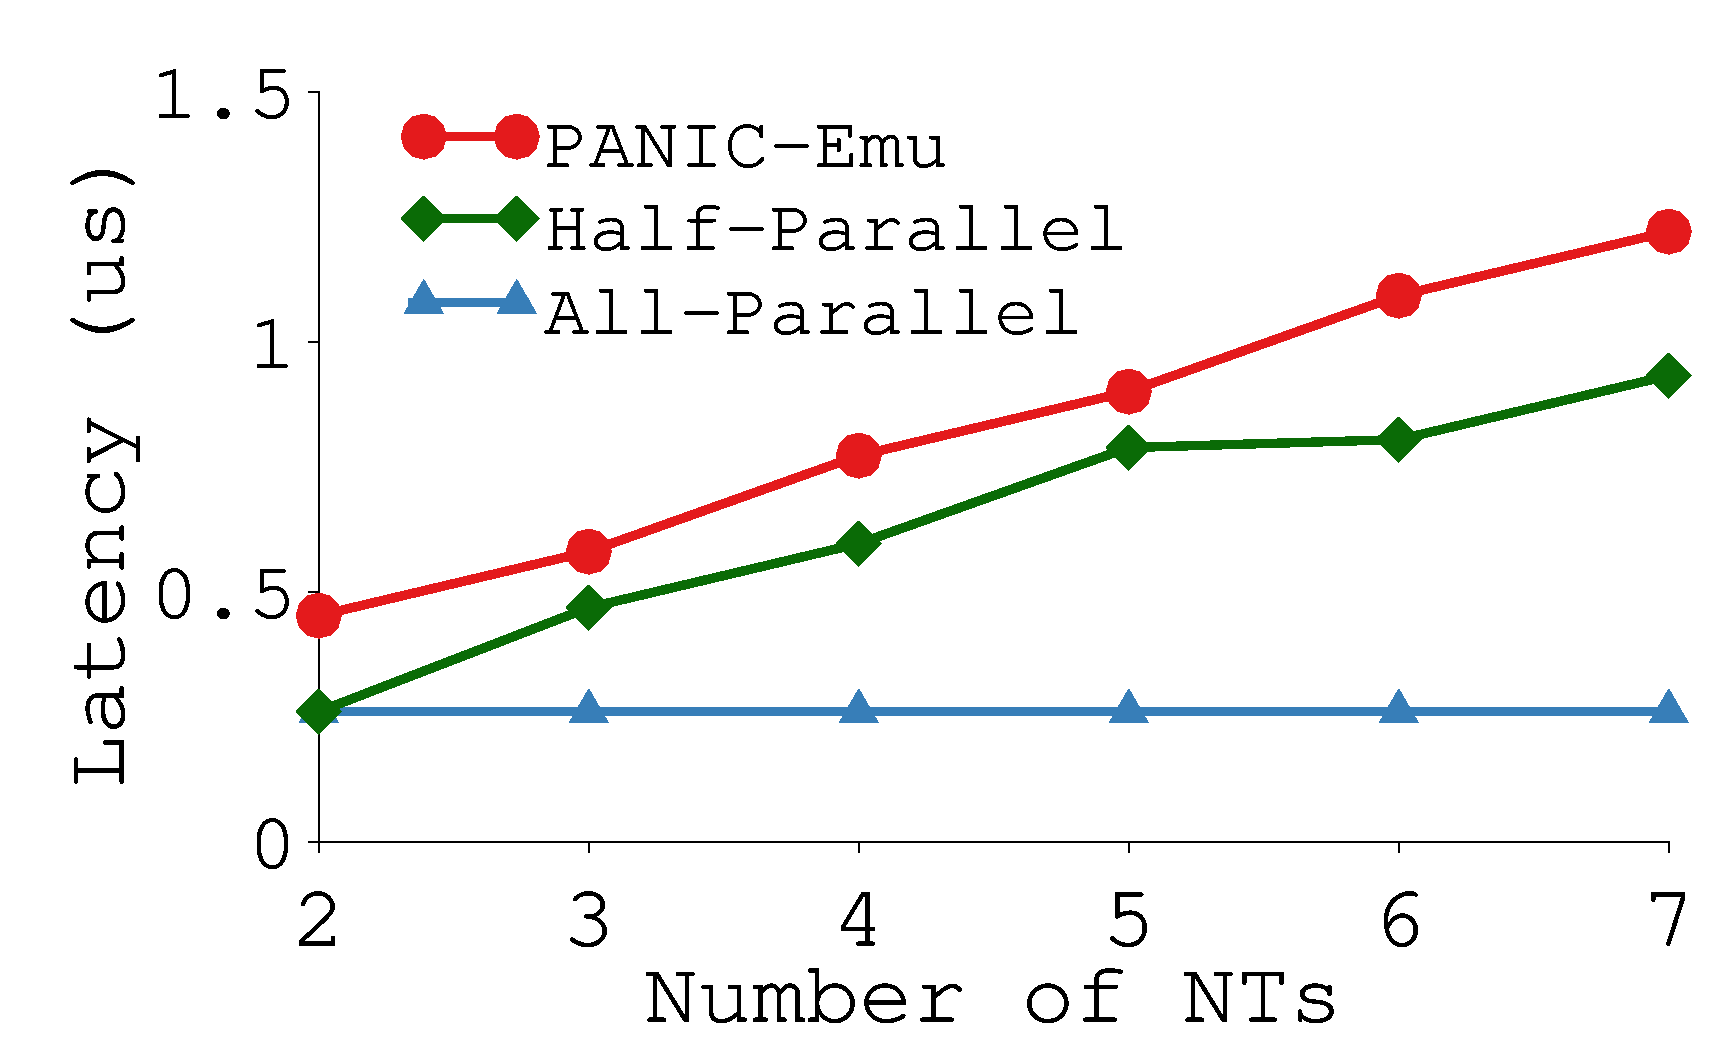
\includegraphics[width=0.5\textwidth]{snic/Figures/g_plot_nt_parallel.pdf}}
\mycaption{fig-nt-parallel}{\nt{} Parallelism.}
{
}
\end{center}
\end{figure*}
}

\subsection{Deep Dive into \snic\ Designs}
\label{sec:snic:deepdive}

We now perform a set of experiments to understand the implications of \snic's various designs in terms of performance and OpEx cost, also with the Facebook distribution.
%We calculate OpEx cost as the amount of and duration of hardware resources used. 
%For these experiments, we generate workloads also from the same Facebook distributions.

\bolditpara{Effect of auto-scaling.}~~
We compare our auto-scaled implementation of \snic\ with two types of static allocations (\ie, no load-based scaling): allocating for the highest load needs ({\em static-max}) and allocating for the average load needs ({\em static-avg}), and an unrealistic auto-scaled scheme which instantly scales the right amount of \nt\ instances as load changes and incurs zero context switching overhead ({\em as-instant}).
We generate two workloads using the Facebook distributions, one where different endpoints spike at similar time (high correlation) and one where they spike at different times (low correlation).
Figure~\ref{fig-sim-overview} shows the performance slowdown (compared to no network disaggregation) and OpEx costs (compared to static-max).

\snic\ is at the Pareto frontier compared to the two static allocation schemes. Static-max has the best performance but the worst OpEx cost, as it pays for the peak hardware resources for the entire duration. In contrast, static-avg has the worst performance but best OpEx cost, since it only allocates the resource for the average usage for the entire duration.
Compared to \snic, as-instant only achieves slightly better performance with slightly more OpEx spending, as it tightly matches resources to the load which is unrealistic.

Comparing the two workloads, the low-correlation one always has better performance and more OpEx spending than the high-correlation one (except for as-instant which always yields best performance and static-max which always yields best performance and worst OpEx).
This is because with low correlation, the aggregated traffic is more flattened out, which gives \snic\ better chance to properly handle. As a result, \snic\ scales the right amount of resources to satisfy the load's performance needs.
When correlation is high (which is unlikely from our trace analysis in \S\ref{sec:snic:benefits}), there will be fewer but more intensive spikes. When \snic\ is not fast or powerful enough to handle some of them, less resources is used but the performance goes down.

\bolditpara{Effect of victim cache.}~~
To evaluate the effect of our victim-cache design, we set the baseline to be disabling victim cache (blue dot in Figure~\ref{fig-sim-single-snic}).
We then change how often a de-scheduled \nt\ can be kept around as a victim instead of being completely deleted (shown as percentage on the green line). 
This configuration models how often an \snic's area is free to host victim \nt{}s.
As expected, the more de-scheduled \nt{}s we can keep around, the better performance we achieve, with no victim cache (baseline) having the worst performance.
The OpEx implication is less intuitive.
Here, we only count the time and amount of \nt\ regions that are actually accessed, as only those will cause the dynamic power (when idle, FPGA has a static power consumption regardless of how it is programmed).
With fewer de-scheduled \nt{}s kept around, more \nt{}s need to be re-launched (through FPGA PR) when the workload demands them. 
These re-launching overhead causes the OpEx to also go up.

\bolditpara{Effect of area over-commitment.}~~
We change the degree of area over-commitment by limiting how much hardware resources (\ie, NT regions) the workload can use compared to the ideal amount of resources needed to fully execute it.
%which is the amount of resources actually used over the total amount of hardware resources needed to execute the workload without context switching.
As Figure~\ref{fig-sim-single-snic} shows, as we increase the area over-commitment rate, we see worse performance and less resources (OpEx) used. 
Thus, our design uses distributed \snic{}s to avoid the over-commitment of a single \snic.

\bolditpara{\nt\ chaining.}~~
To evaluate the effect of \snic's \nt-chaining technique, we change the length of \nt\ sequence from 2 to 7 (as prior work found real NFs are usually less than 7 in sequence~\cite{NFP-sigcomm17}).
In comparison, we implemented PANIC's scheduling mechanism on our platform, so that everything else is the same as \snic.
We also evaluate the case where \snic\ splits the chain into two sub-chains.
Figure~\ref{fig-nt-chain} shows the total latency of running the \nt\ sequence with these schemes.
\snic\ outperforms PANIC because it avoids going through the scheduler during the sequence for single-chain and only goes through the scheduler once for half-chain.

{
\begin{figure*}[t]
\begin{center}
\centerline{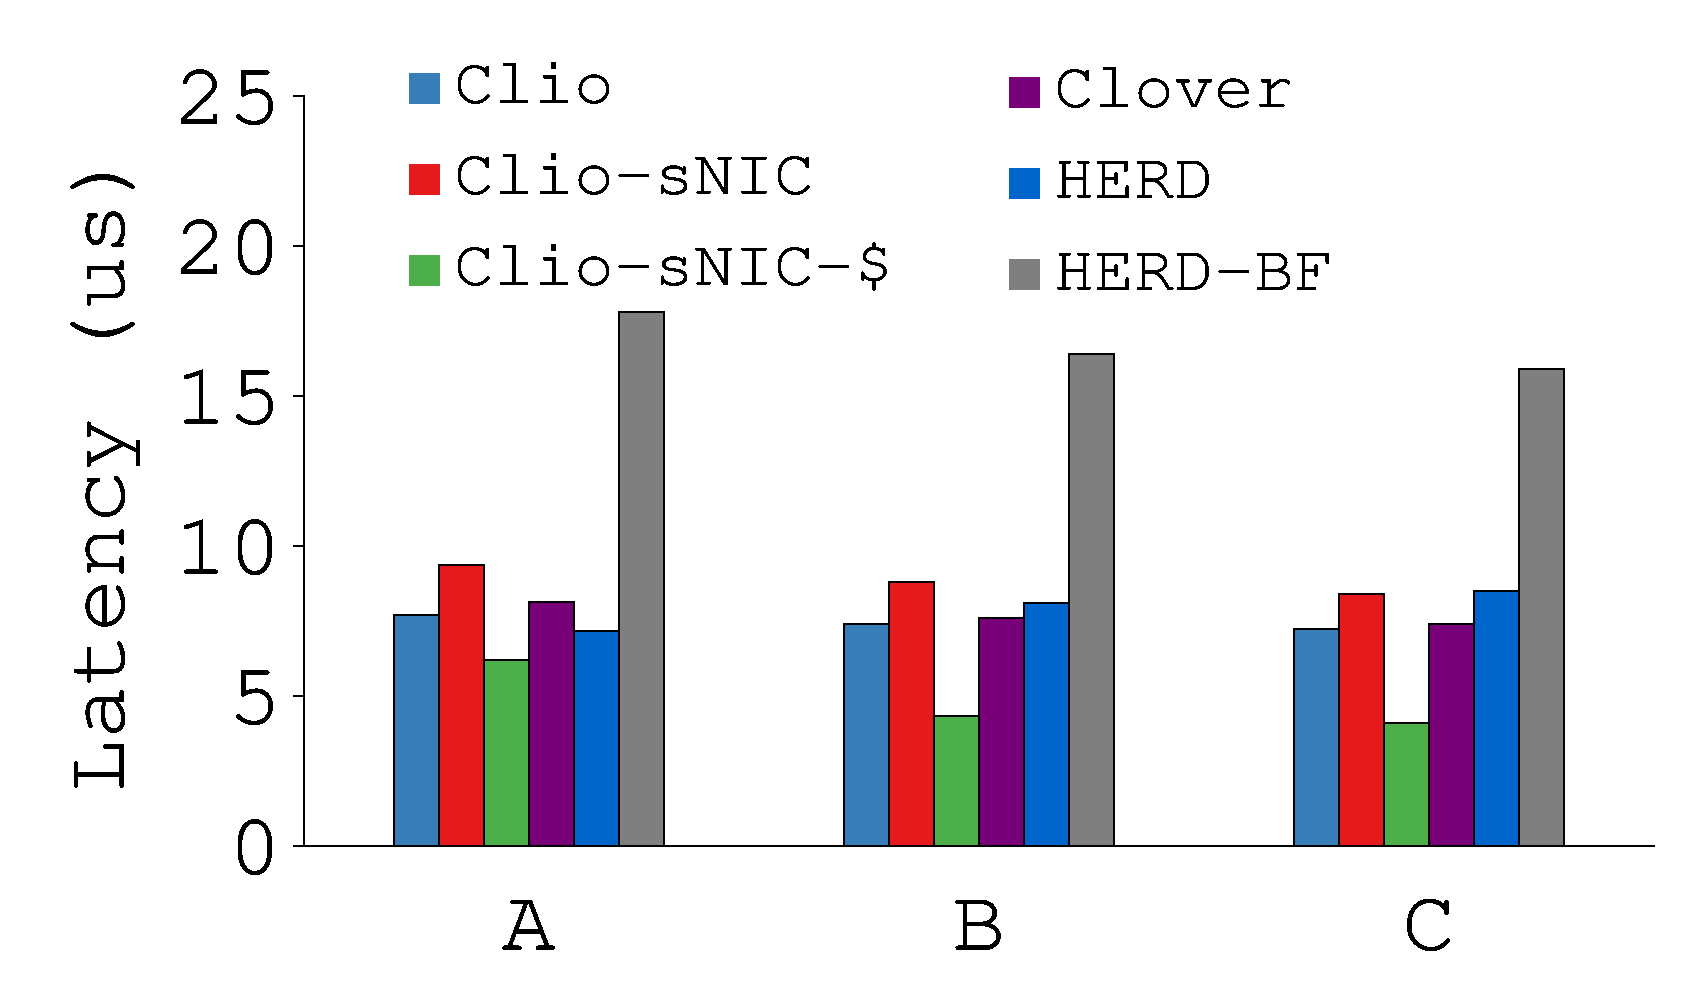
\includegraphics[width=0.5\textwidth]{snic/Figures/g_plot_ycsb.pdf}}
\mycaption{fig-snic-ycsb}{YCSB Latency.}
{
}
\end{center}
\end{figure*}
}
{
\begin{figure*}[h]
\begin{center}
\centerline{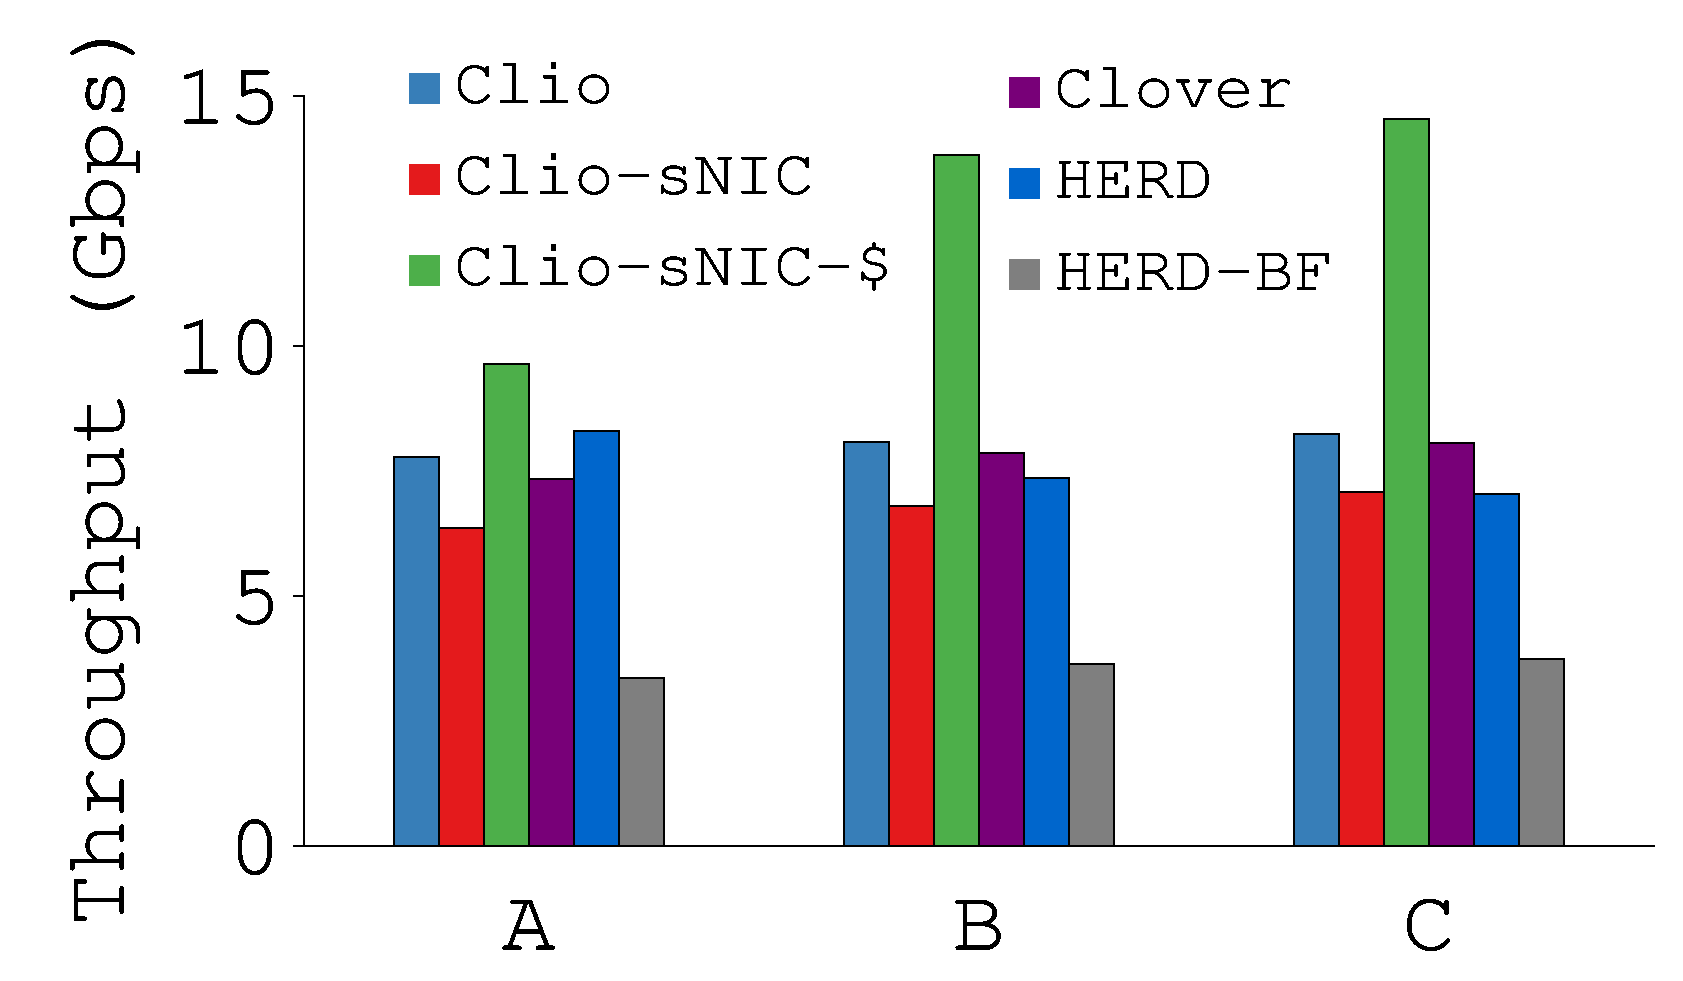
\includegraphics[width=0.5\textwidth]{snic/Figures/g_plot_ycsb_throughput.pdf}}
\mycaption{fig-snic-ycsb-tput}{YCSB Throughput.}
{
}
\end{center}
\end{figure*}
}
{
\begin{figure*}[h]
\begin{center}
\centerline{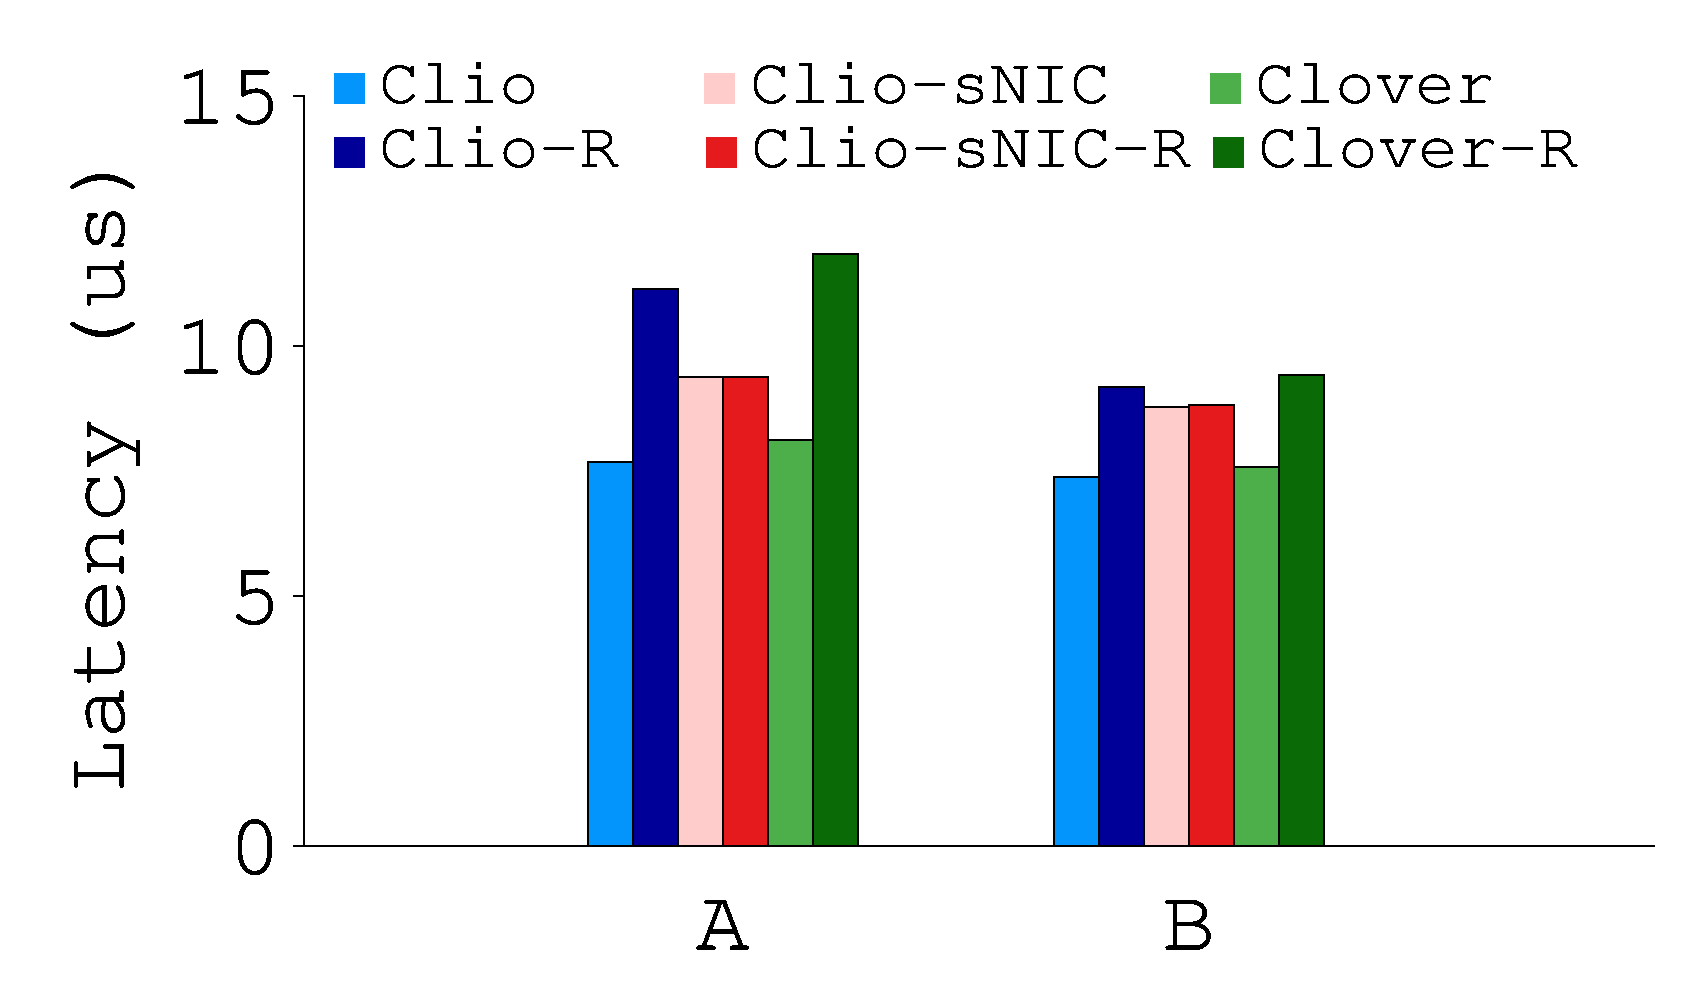
\includegraphics[width=0.5\textwidth]{snic/Figures/g_plot_ycsb_replication.pdf}}
\mycaption{fig-ycsb-replication}{Replicated YCSB.}
{
}
\end{center}
\end{figure*}
}
{
\begin{figure*}[h]
\begin{center}
\centerline{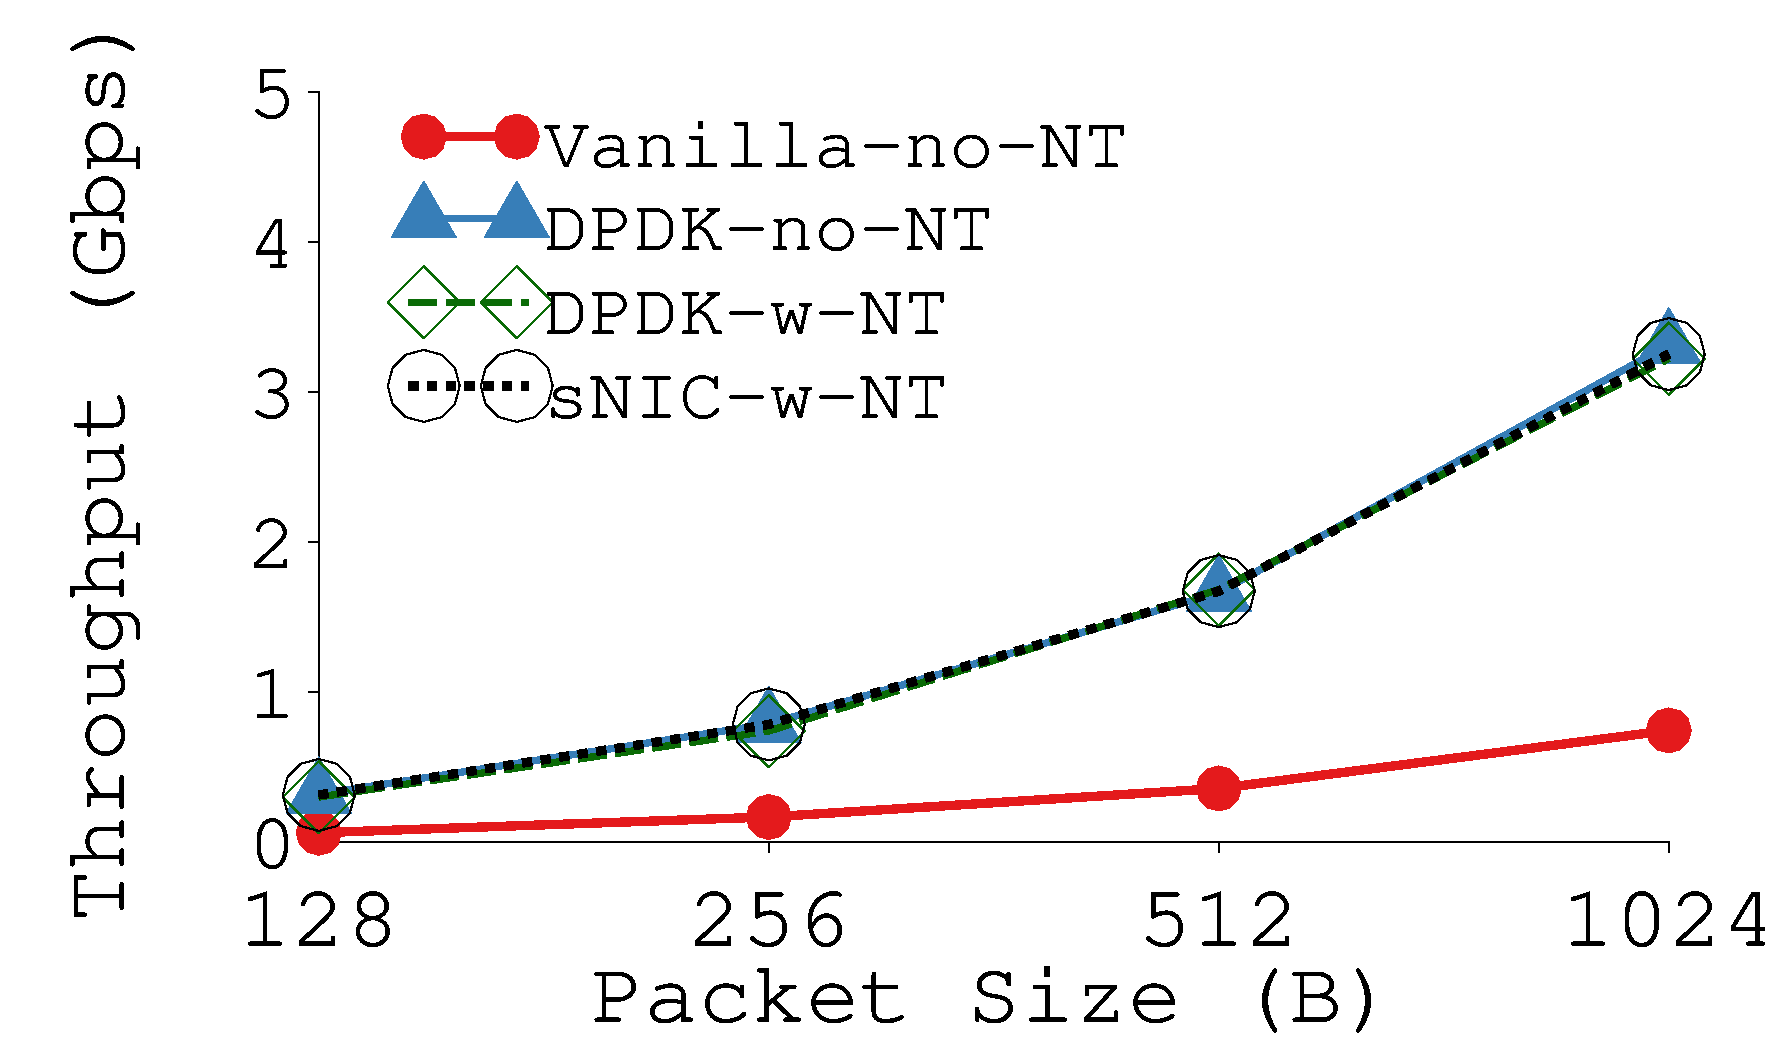
\includegraphics[width=0.5\textwidth]{snic/Figures/g_plot_ovs.pdf}}
\mycaption{fig-ovs}{VPC Performance.}
{
}
\end{center}
\end{figure*}
}

{
\begin{figure}[th]
\begin{center}
\centerline{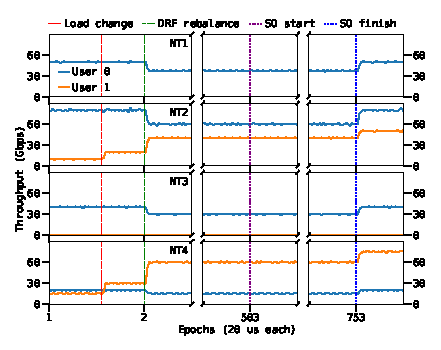
\includegraphics[width=\textwidth]{snic/Figures/drf.pdf}}
\mycaption{fig-drf}{\nt{} Scheduling.}
{
SO: Scaling Out.
}
\end{center}
\end{figure}
}

\bolditpara{\nt-level parallelism.}~~
We then evaluate the effect of \snic's \nt-level parallelism by increasing the number of \nt{}s that could run in parallel.
We compare with PANIC (on our platform), which does not support \nt-level parallelism.
We also show a case where we split \nt{}s into two groups and run these groups as two parallel \nt-chains (half-parallel).
Figure~\ref{fig-nt-parallel} shows the total latency of these schemes.
As expected, running all \nt{}s in parallel achieves the best performance.
The tradeoff is more \nt\ region consumption.
Half-parallel only uses two regions and still outperforms the baseline. % no parallelism PANIC scheme.

\bolditpara{DRF Fairness.}~~
To evaluate the effectiveness of our scheduling policy, we ran the synthetic workloads as described in Figure~\ref{fig-nt-example} and use the default \texttt{EPOCH\_LEN} of 20\mus\ and \texttt{MONITOR\_PERIOD} of 10\ms.
%Here, we set \texttt{EPOCH\_LEN} to 20\mus\ and \texttt{MONITOR\_PERIOD} to 10 epochs or 200us.
Figure~\ref{fig-drf} shows the resulting throughput timeline for different \nt{}s of the two users.
In between epoch 1 and 2, the loads of user2 increased to the second step.
At the next epoch, we run DRF and adjust the allocation. After the DRF algorithm finishes (in around 3\mus), user2 gets a higher (and fairer) allocation of \nt{}2 and \nt{}4, while user1's allocation decreases.
After observing \nt{}2 being overloaded for 10\ms, the \snic\ scales out \nt{}2 by adding one more instance of it at time epoch-503.
After PR is done (in 5\ms), both user1 and user2's throughput increase.



\subsection{End-to-End Application Performance}

We now present our end-to-end application performance conducted on our rack testbed. Because of space constraint, \textit{we move the consolidation experiments of these applications to the Appendix}.

\subsubsection{Disaggregated Key-Value Store}

In this set of experiments, we use one client server and two Clio devices. The Clio devices connect to one \snic\ which connects to the ToR switch. We run YCSB's workloads A (50\% set, 50\% get), B (5\% set, 95\% get), and C (100\% get)~\cite{ycsb-socc10} for these experiments. We use 100K key-value entries and run 100K operations per test, with YCSB's default key-value size of 1\KB\ and Zipf accesses ($\theta=0.99$). 
%The accesses to keys follow the Zipf distribution ($\theta=0.99$).

\bolditpara{Non-replicated YCSB performance and caching.}~~
%Our disaggregated key-value store experiments build on top of the Clio disaggregated memory platform~\cite{clio-arxiv}, where the client side is a regular server and the memory side is two Clio boards.
%Our baseline is the original Clio, which runs a Go-back-N transport on the Clio boards.
%With \snic, we first move the Go-back-N transport as an \nt\ to the \snic\ which connects the two Clio boards to the ToR switch.
%We then add a caching \nt\ to the \snic.
We first evaluate the performance of running YCSB without replication using one client server and one Clio memory device.
Figure~\ref{fig-snic-ycsb} and \ref{fig-snic-ycsb-tput} plot the average end-to-end latency and throughput of running the YCSB workloads with (1) the original Clio, (2) Clio's Go-Back-N transport offloaded to \snic\ (Clio-sNIC), (3) adding caching on top of Clio-sNIC (Clio-sNIC-\$), (4) Clover~\cite{Tsai20-ATC}, a {\em passive} disaggregated memory system where all processing happens at the client side and a global metadata server, (5) HERD~\cite{Kalia14-RDMAKV}, a two-sided RDMA system where both the client and memory sides are regular servers, and (6) HERD running on the NVidia BlueField SmartNIC~\cite{bluefield-nic} (HERD-BF).
\snic's performance is on par with Clio, Clover, and HERD, as it only adds a small overhead to the baseline Clio.
With caching \nt, \snic\ achieves the best performance among all systems, esp. on throughput. 
This is because all links in our testbed are 100\Gbps\ except for the link to the 10\Gbps\ Clio boards. When there is a cache hit at the \snic, we avoid going to the 10\Gbps\ Clio boards.
HERD-BF performs the worst because of the slow link between its NIC and the ARM processor.

\bolditpara{Replicated YCSB performance.}~~
%As many key-value store users desire strong reliability, replication at the memory nodes is usually required.
We then test Clio, Clover, and Clio with \snic\ with replicated write to two Clio devices. HERD does not support replication, and we do not include it here.
Clover performs replicated write in a similar way as the baseline Clio, but with a more complex protocol.
Figure~\ref{fig-ycsb-replication} plots the average end-to-end latency with and without replicated writes using the YCSB A and B workloads.
With \snic's replication \nt, the overhead that replication adds is negligible,
while both Clio and Clover incur significant overheads when performing replication.

\subsubsection{Virtual Private Cloud}
We use one sender server and one receiver server, both running Open vSwitch (OVS)~\cite{ovs-nsdi15}, to evaluate VPC.
Our baseline is the default Open vSwitch that runs firewall, NAT, and AES.
We further improve the baseline by running DPDK to bypass the kernel.
In the \snic\ setup, we connect the sender to an \snic\ and the receiver to another \snic.
Each \snic\ runs the three NFs as a chain.
Figure~\ref{fig-ovs} shows the throughput results.
Overall, we find OVS to be a major performance bottleneck in all the settings. Using DPDK improves OVS performance to some extent.
Compare to running \nt{}s at servers, offloading them to the \snic\ improves throughput, but is still bounded by the OVS running at the endhosts.
\section{Conclusion}
\label{sec:snic:conclude}

We propose network disaggregation and consolidation by building SuperNIC, a new networking device specifically for a disaggregated datacenter.
Our FPGA prototype demonstrates the performance and cost benefits of \snic.
Our experience also reveals many new challenges in a new networking design space that could guide future researchers.

\section{Acknowledgments}
Chapter 5, in part, has been submitted for publication of the material as it may appear in Yizhou Shan, Will Lin, Ryan Kosta, Arvind Krishnamurthy, Yiying Zhang, ``Disaggregating and Consolidating Network Functionalities with SuperNIC'', \textit{arXiv, 2022}. The dissertation author was the primary investigator and author of this paper.
\if 0

\clearpage

\appendix

\section{Appendix}

\subsection{FPGA Resource Utilization}

The following table shows the FPGA resources used by \snic{} shell.
Most of the resources are left for running \nt{}s.

\begin{center}
\scriptsize
\begin{tabular}{ p{0.6in} | p{0.2in} |p{0.27in} }
 & \textbf{Logic} & \textbf{Memory} \\
\textbf{Module} & \textbf{(LUT)} & \textbf{(BRAM)} \\
\hline
\hline
%Firewall     & 2.8\% & 0.5\% \\
%AES-256       & 0.4\% & 0 \\
%Transport    & 1.3\% & 0.42\% \\
%\hline
%\hline
\snic{} Core & 4.36\%   & 4.74\% \\
Packet Store & 0.91\%   & 9.17\% \\
PHY+MAC      & 0.72\%   & 0.35\% \\
DDR4Controller         & 1.57\%   & 0.29\% \\
MicroBlaze   & 0.25\%   & 1.81\% \\
Misc         & 1.52\%   & 0.75\% \\
%\textbf{Total (w/o \nt{})}        & \textbf{9.33\%}   & \textbf{17.11\%} \\
\hline
\textbf{Total}        & \textbf{9.33\%}   & \textbf{17.11\%} \\
\end{tabular}
\end{center}



\subsection{Cost Calculation}
We explain the different deployment models and the cost calculation formulas behind our CapEx comparisons.
We limit our scope to rack-scale as the higher-level network hierarchies
are orthogonal to the resource pool deployment models.
We calculate that, to deploy a certain number of endpoints, what's the
network cost (i.e., the network interface card, cable, and switch port costs).

We compare the following models:
1) Non-disaggregation model, or the traditional model, termed \texttt{traditional}.
2) Disaggregation model, in which we insert the network pool between endpoints and the ToR switch (Figure~\ref{fig-topology} (a)), termed \texttt{ring}.
3) Disaggregattion model, in which we connect the pool of network devices directly to the ToR switch (Figure~\ref{fig-topology} (b)), termed \texttt{direct}.
For both disaggregation models, we further compare two type of devices: sNIC which has auto-scaling capability and multi-host NIC which can only provision for max resource usage. With runtime dynamic scaling and load balancing features, sNICs can provision for less than the max required resource , the specific ratio is calculated by comparing a particular workload's the sum-of-peak versus the peak-of-sum.

In all, we have the following models under comparison:
\texttt{traditionl, sNIC-direct, sNIC-ring, mhnic-direct, mhnic-ring}.

We now detail the cost calculations.
In the traditional non-disaggregation model,
each endpoint has a full-fledged NIC and a normal high-speed cable for connection to the ToR switch.
In both disaggregation models, since most network tasks are offloaded to the network resource pool, each endpoint can uses a down-scaled NIC.
Furthermore, the last hop link layer between endpoints and the network resource pool is reliable, we can leverage down-scaled, cheaper and less reliable physical cable~\cite{RAIL-NSDI}.

We use the following parameters in our calculation:
\begin{itemize}
\item Deploy \texttt{N} devices.
\item Each switch port has a cost of \texttt{costSwitchPort}
\item A full-fledged NIC's cost is \texttt{costNIC}. A down-scaled NIC cost is \texttt{costDSNIC}.
\item A normal high-speed cable cost is \texttt{costCable}.
A down-scaled less reliable physical cable cost is \texttt{costDSCable}.
\item A consolidation ratio \texttt{consolidRatio} determines how many endpoints are sharing one network resource pool device. We can calculate the number of network pool devices by \texttt{M = N / consolidRatio}.
\item For a network device, only a certain portion is dedicated to running network task, other parts are used as shell. We define the cost ratio used by network task to be \texttt{NTCostRatio}.
\item The peak-of-sum versus the sum-of-peak yields the auto-scaling potentials. A multi-host NIC (mhnic) provisions for the sum-of-peak while an sNIC provisions for the peak-of-sum. We call this ratio \texttt{capExConsolidRatio}.
\item The multi-host NIC's cost can be calculated as \texttt{costMHNIC = costNIC * N}.
\item The sNIC's cost can be calculated as \texttt{costsNIC = costMHNIC * capExRatio}, in which \texttt{capExRatio = (1 - NTCostRatio) + NTCostRatio * capExConsolidRatio}.
\end{itemize}

We now define each model's cost.

The traditional deployment model's cost is straightforward, it includes NIC, cable and switch ports:
\begin{gather}
N * (costNIC + costCable + costSwitchPort)
\end{gather}

The disaggregation models' cost has more moving parts than the traditional. It includes the down-scaled NICs and cables, network pool devices, the cables to the ToR switch, and switch ports.

The first disaggregation model (Figure~\ref{fig-topology} (a)) can be calculated as follows (for both \texttt{sNIC-ring, mhnic-ring}). 
\begin{align}
N * (costDSNIC + costDSCable) + \\
M * (costsNIC + costCable + costSwitchPort)
\end{align}

The second disaggregation model (Figure~\ref{fig-topology} (b)) can be calculated as follows (for both \texttt{sNIC-direct, mhnic-direct}).
\begin{align}
N * (costDSNIC + costCable + costSwitchPort) + \\
M * (costsNIC + costCable + costSwitchPort)
\end{align}

This tables shows the real-world numbers we use.

\begin{center}
\scriptsize
\begin{tabular}{|l|l|l|} 
 \hline
 Parameters & Value & Note \\
 \hline\hline
 costSwitchPort & \$250 & FS 100Gbps switch~\cite{fs-64port-switch} \\
 costNIC & \$500 & Mellanox Connect-X5 \\
 costCable & \$100 & FS DAC 100Gbps cable \\
 costDSNIC & costNIC * 0.2 & Numbers from our prototpe \\
 costDSCable & costCable * 0.6 & ~\cite{RAIL-NSDI} \\
 consolidRatio & 4 & Current model\\
 NTCostRatio & 0.9 & Numbers from our prototype \\
 capExConslidRatio & 0.23 & Facebook Hadoop trace~\cite{facebook-sigcomm15} \\
 \hline
\end{tabular}
\end{center}

%\subsection{Extended Evaluation Results}

{
\begin{figure*}[th]
\begin{minipage}{\figWidthSix}
\begin{center}
\centerline{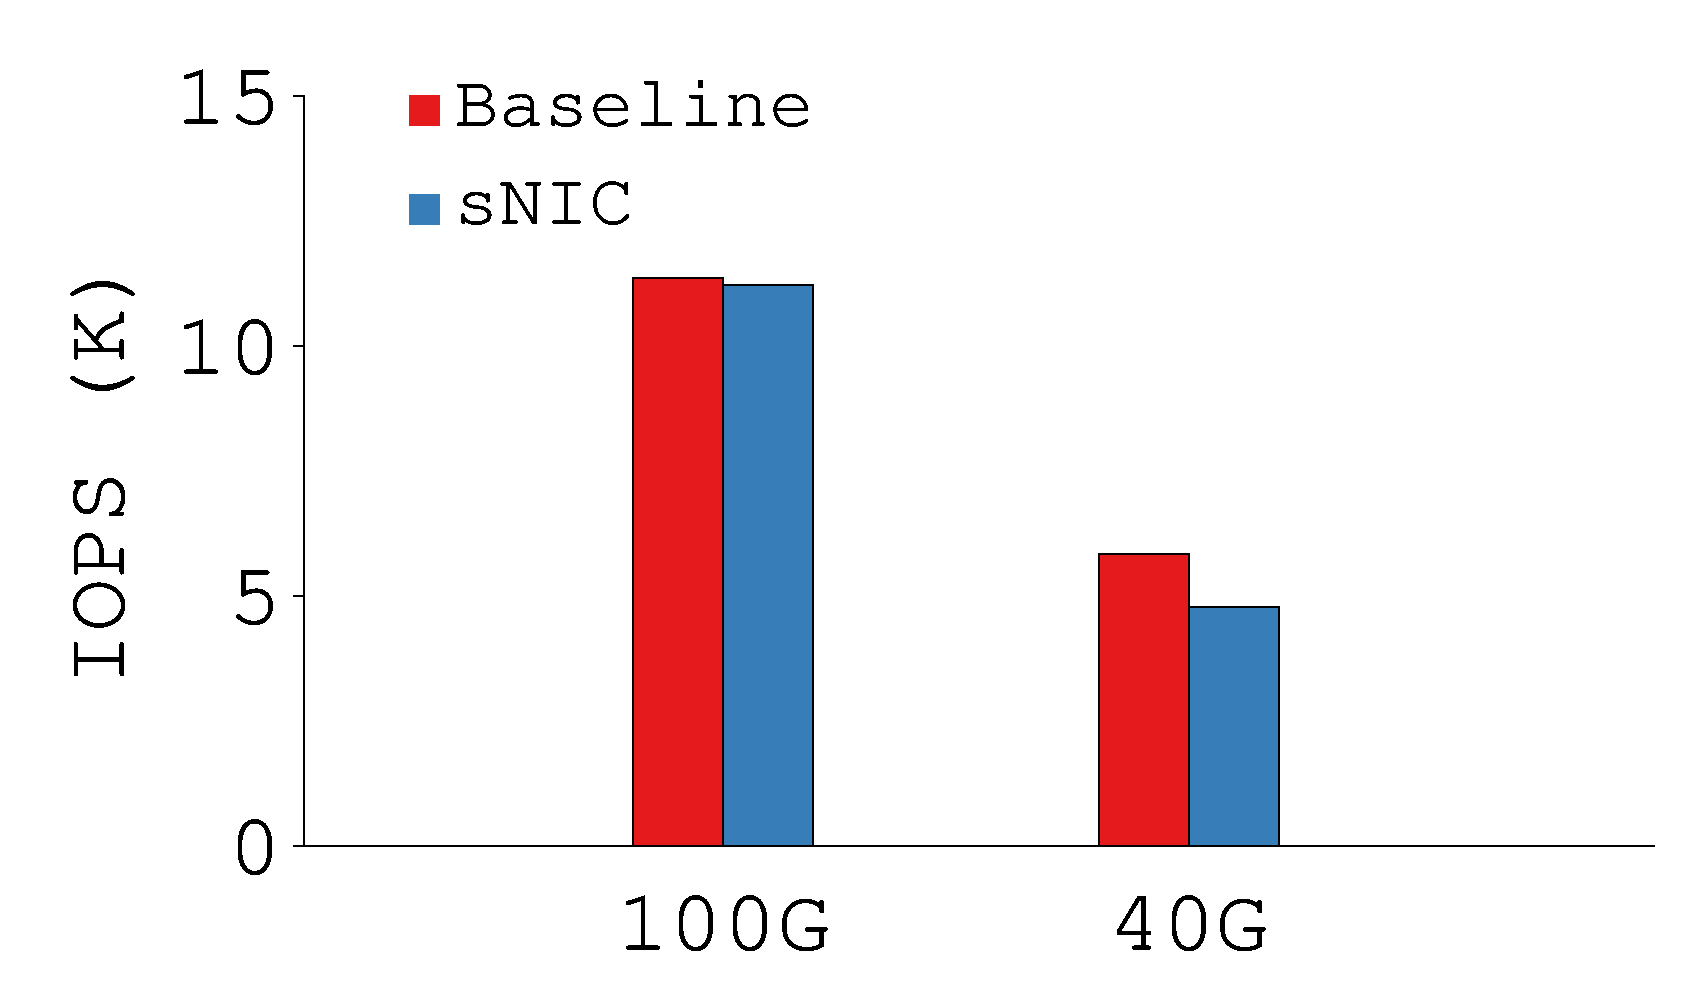
\includegraphics[width=\columnwidth]{Figures/g_plot_conslid_perf.pdf}}
\vspace{-0.1in}
\mycaption{fig-kv-consolid}{Consolidation Performance w/ FB Key-Value.}
{
}
\end{center}
\end{minipage}
\begin{minipage}{\figWidthSix}
\begin{center}
\centerline{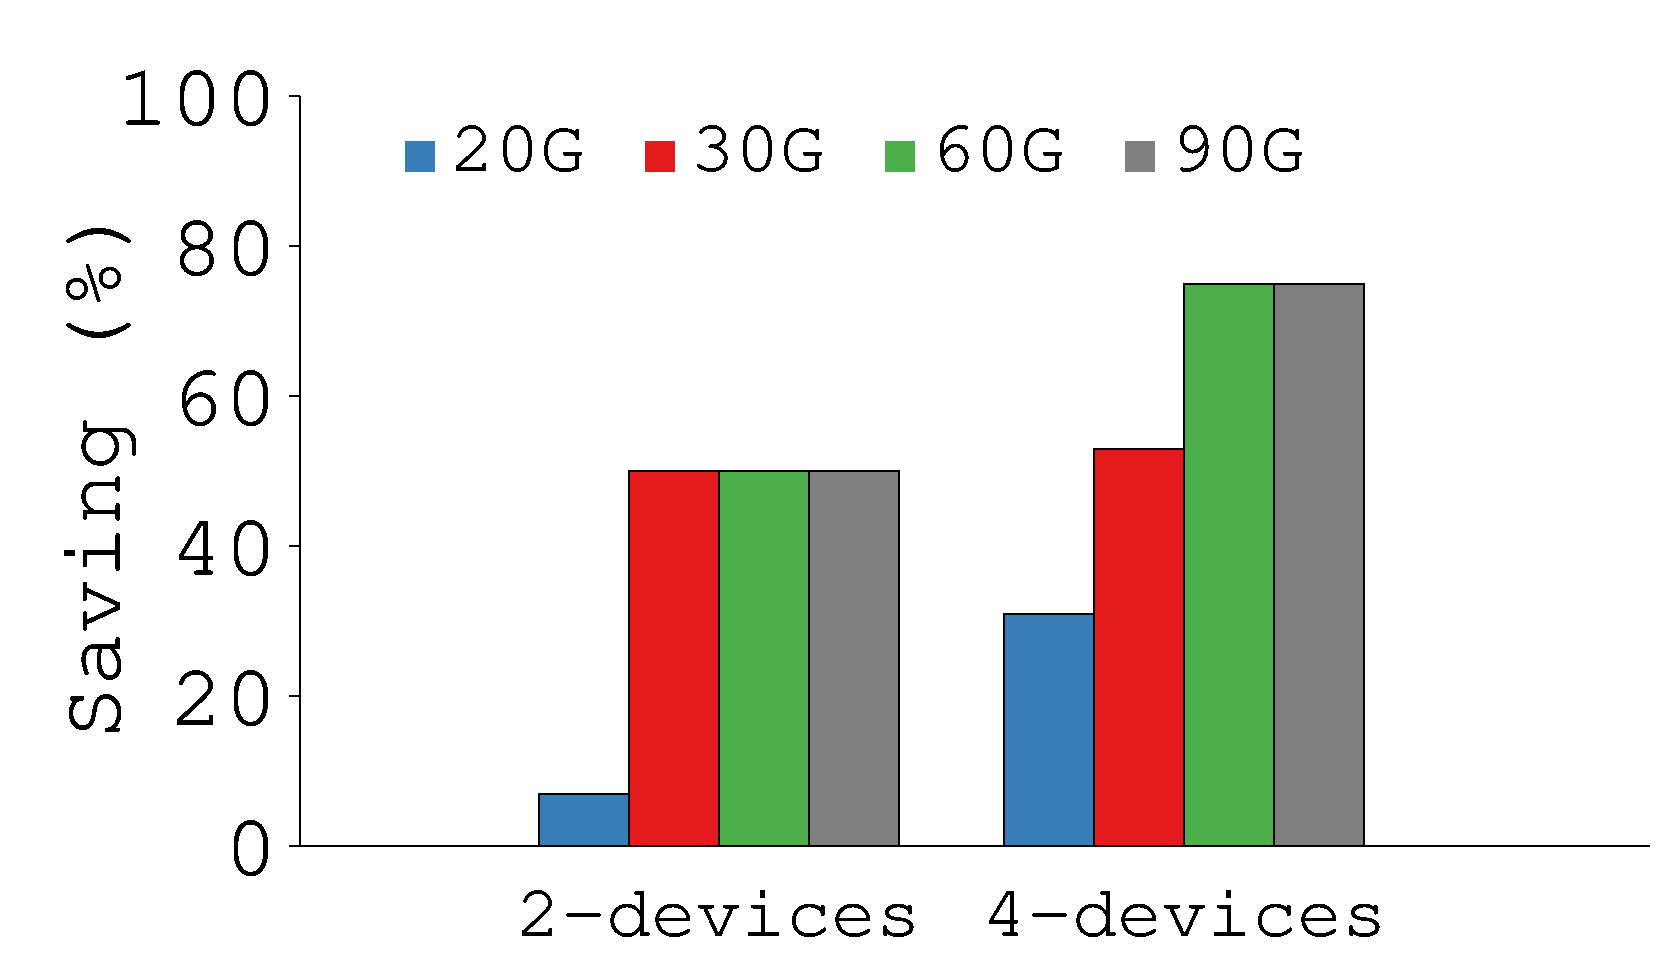
\includegraphics[width=\columnwidth]{Figures/g_plot_conslid_cost.pdf}}
\vspace{-0.1in}
\mycaption{fig-kv-cost}{Consolidation Resource Usage w/ FB KV.}
{
}
\end{center}
\end{minipage}
\vspace{-0.1in}
\end{figure*}
}
\subsection{End-to-End Application Performance and Cost with Consolidation}

To evaluate the benefit and tradeoff of consolidation, we deploy a testbed with four sender and four receiving servers with four setups:
each endhost connects to a ToR switch with 100\Gbps\ or 40\Gbps\ link (baseline, no consolidation), and four endhosts connect to an \snic, each with 100\Gbps\ or 40\Gbps\ link, and the \snic\ connects to the ToR switch with a 100\Gbps\ or 40\Gbps\ link (\snic\ consolidation).
%, and 3) four endhosts connect to an emulated multi-host NIC, each with a 25\Gbps\ link (\S\ref{sec:related}), and the multi-host NIC connects to the ToR switch with a 100\Gbps\ link. %(multi-host NIC, statically partitioned link bandwidth).
For both settings, we execute two \nt{}s, firewall and NAT, in FPGA. 
For the baseline, each endhost has its own set of \nt{}s, while %the multi-host NIC uses one set of \nt{}s in total and 
\snic\ autoscales \nt{}s as described in \S\ref{sec:policy}.
On each server, we generate traffic to follow inter-arrival and size distribution reported in the Facebook 2012 key-value store trace~\cite{Atikoglu12-SIGMETRICS}.
%the Hadoop load distribution reported in the 2015 Facebook workloads~\cite{facebook-sigcomm15}.
%Since there is no reported inter-arrival time for these workloads, we use the inter-arrival time reported by the 2012 Facebook workloads~\cite{Atikoglu12-SIGMETRICS}.
%We measure the application throughput (IOPS) every 10\ms\ time unit to evaluate the throughput changes over time.

Figure~\ref{fig-kv-consolid} reports the throughput comparison of \snic\ and the baseline.
%average IOPS and 95-percentile IOPS across all time units for the three settings. 
\snic\ only adds 1.3\% performance overhead to the baseline under 100\Gbps\ network and 18\% overhead under 40\Gbps\ network. 
We further analyze the workload and found its median and 95-percentile loads to be 24\Gbps\ and 32\Gbps.
With four senders/receivers, the aggregated load is mostly under 100\Gbps\ but often exceeds 40\Gbps.
Note that a multi-host NIC would not be able to achieve \snic's performance, as it subdivides the 100\Gbps\ or 40\Gbps\ into four 25\Gbps\ or 10\Gbps\ sub-links, which would result in each endhost exceeding its sub-link capacity.


We then calculate the amount of FPGA used for running the \nt{}s multiplied by the duration they are used for, to capture the run-time resource consumption with \snic's autoscaling mechanism. The baseline has one set of \nt{}s per endhost for the whole duration.
Figure~\ref{fig-kv-cost} shows this comparison when consolidating two and four endhosts to an \snic\ and using \nt{}s of different performance metrics.
For a slower \nt{} (\eg, one that can only sustain 20\Gbps\ max load), the \snic\ auto-scales more instances of it, resulting in less cost saving.
Our implementation of firewall \nt{} reaches 100\Gbps, while the AES \nt\ is 30\Gbps, resulting in a 64\% cost saving when deploying both of them.



%On the other hand, multi-host NIC incurs higher performance overhead, especially for the tail.
%Whenever any endhost exceeds 25\Gbps\ load, multi-host NIC will have a bottleneck link.
%On the other hand, \snic\ can sustain the peak of aggregated traffic, which is mostly under 100\Gbps, demonstrating the benefit of run-time, dynamic consolidation.

\if 0
\subsubsection{Distributed \snic{}}
To run an \nt\ at a remote \snic,
an \snic{}'s SoftCore first sends a control message to the remote \snic{} to launch the \nt{} and then installs forwarding rules to its parser. This process takes 2.3\mus\ in our testbed.
Afterwards, packets are forwarded to the remote \snic. We observe an addition of 1.3\mus\ latency when packets go through the remote \snic.
\fi
\fi



\chapter{Conclusion}
TODO.

%% APPENDIX
\appendix
\chapter{Final notes}
What to do about things \cite{Martin_1983}.  What did he say \cite{Rilling_Insel_1999}.
  Remove me in case of abdominal pain.



%% END MATTER
% \printindex %% Uncomment to display the index
% \nocite{}  %% Put any references that you want to include in the bib 
%               but haven't cited in the braces.
\bibliographystyle{alpha}  %% This is just my personal favorite style. 
%                              There are many others.
%\setlength{\bibleftmargin}{0.25in}  % indent each item
%\setlength{\bibindent}{-\bibleftmargin}  % unindent the first line
%\def\baselinestretch{1.0}  % force single spacing
%\setlength{\bibitemsep}{0.16in}  % add extra space between items
\bibliography{template}  %% This looks for the bibliography in template.bib 
%                          which should be formatted as a bibtex file.
%                          and needs to be separately compiled into a bbl file.
\singlespace  %to force bibilography environment to use single spacing for each entry 
              %double spacing between entries remains
\end{document}

